\section{S/B classification} \label{section: s/b classification}

% loss function weights
% Direction for comparisons:
% 		1) architecture
% 		2) input features
% 		3) sample dependency
% 		4) for background from MC weight vs no weights


Now that we have found the optimal model to maximize the pairing efficiency while 
reducing as much as possible the background mass sculpting,
we would like to use SPANet as signal/background (S/B) classifier. We will try different trainings and check if we outperform the DNN used for the Run 2 data presented in the AN (cite). In the following sections, we will compare the performance of our trainings when using different input variables, as well as the sample dependency of the background. Although, we will first delve into some technical details on how to implement the weights for the loss function to use SPANet as classifier.

%Add number of events before/ after preselections

\subsection{Weights for the computation of the loss}

Firstly, in order to use SPANet as classifier, we need to modify the weights for the computation of the loss as we will now be using in the training signal \textbf{and} background events. The sample we will use for the signal events is the same as the one in section \ref{section: improving}.  For the background, we would ideally like to work with morphed 4b data. Unfortunately, we don't have access to this background so we will be using the following ones:
\begin{itemize}
	\item 2b data
	\item 2b QCD Montecarlo (MC)
    \item 4b QCD Montecarlo (MC)
\end{itemize}
As we are now using signal{and} background events, it is important to take into account that the number of events are not the same for the different processes. To do so, we will introduce the {Event weights} and the {Class weights}, that we will explain in the following sections.

%Therefore, to avoid imbalanced data classification problems, we will weight our loss function accordingly.

\subsubsection{Event weights}

The QCD MC and signal events, as the name implies, are MC simulations. When generating these simulations we use the theoretical cross section given by the SM. Nevertheless, with enough computational power it is possible generate as many events as we want of that particular process, which does not necessarily match the number of events in our detector.
%as the luminosity is not taken into account. 
Or, if a process is very computationally expensive we can't generate enough simulations that will match the number of events in real data. This is why,  Event weights are usually introduced to rescale the number of events of our process.

In the detector, the expected number of events of a process with cross section $\sigma$ will be given by (cite?):

\begin{equation*}
    N_{\text{exp}} = \lumi \times \sigma \times \epsilon
\end{equation*}

\noindent With $N_{\text{exp}}$ being the total number of expected events in the detector, $\sigma$ the cross-section of this process, \lumi the integrated luminosity and $\epsilon$ the efficiency defined as follows (cite?):

%https://ipnp.cz/scheirich/?page_id=292

\begin{equation*}
    \epsilon= N_{\text{reco}} / N_{\text{gen}}
\end{equation*}

\noindent Where $N_{\text{reco}}$ is the number of events reconstructed in the detector that pass the event selections we defined, and $N_{\text{gen}}$ is the total number of generated events.

If we use directly the number of events from the MC production for our analysis we are implying that $N_{\text{exp}}=N_{\text{reco}}$, which is incorrect as $N_{\text{reco}}$ coming from the MC simulation is arbitrary. In order to match this value to the actual value of events we would observe in the detector, we need to multiply $N_{\text{reco}}$ by a corresponding weight. When we write the number of expected events as follows:

\begin{equation*}
    N_{\text{exp}} = \lumi \times \sigma \times \frac{N_{\text{reco}}}{N_{\text{gen}}}
\end{equation*}

\noindent the expression of the weight becomes clear:

\begin{equation*}
    \text{Event weights} = \frac{\lumi \times \sigma}{N_{\text{gen}}}
\end{equation*}

However, in practice the expression of these weights can vary if we take into consideration Next to Leading Order (NLO) corrections to our process. In this case, most MC generators produce events that already have a weight that is different from 1, called generator-level weights $w_g$.
% because of the way how the MC integration is implemented in the generator)
Hence, the formula for our Event weights per event $i$ is modified as follows:

\begin{equation*}
    \text{Event weights}^i = \lumi \times \sigma \times \frac{w_g^i}{\sum_i w_g^i}
\end{equation*}

For the signal events, the Event weights are all equal up to a sign, but for the background events these are all different.
This definition of Event weights can be then used to match the number of events MC produced and the ones observed in data. However, in the following, we want to use these weights to take into account the MC production effects in the loss. Therefore, since the luminosity is just a constant number that is the same for signal and background, and our aim is not to equalize the number of events to data but to use these weights in the computation of the loss, we will not consider it in Eq.(\ref{eq: event weights}) as it is only a linear rescaling of the value of the weight.

One last point we need to take into consideration for the definition of the Event weights we will use is that the production of the QCD background is divided into $H_T$ bins. Therefore each $H_T$ bin has the same number of events and this would give us a flat distribution of the background. But this is not physical, as in reality we have a falling distribution. To take this into account, we will rescale as a function of $H_T$ bins as follows:

\begin{equation}
	\text{Event weights}^i_j =\frac{w_g^i}{\sum_j w_g^j} \times \frac{\sigma^j}{\sum_{j\in S,B}(\sigma^j)}
 \label{eq: event weights}
\end{equation}
\noindent where $\sigma$ is the cross section of the process per $H_T$ bin $j$. 

When using Eq.(\ref{eq: event weights}),  for signal events we always consider the same process hence the $\sigma$ ratio is equal to 1:
\begin{equation*}
	\frac{\sigma_S^j}{\sum_{j\in S}(\sigma_S^j)}=1
\end{equation*}

For the background we have different values of the cross-section per $H_T$ bin as we are considering many different QCD processes in the same sample, each of them having a different $\sigma$.

\vspace{0.1 cm}

\noindent Ultimately, as an example, we give the following values for the Event weights:

\begin{itemize}
    \item $\text{Event weight for signal per event} \sim 10^{-3}$
    \item $\text{Event weight for 4b-QCD per event} \sim 10^{-5}-10^{-9}$
\end{itemize}

However, a new problem arises as for signal events the weights are much larger than for background events. To give an example, if we compute the total loss as follows :

\begin{equation}
    L_{\text{tot}}= \sum_{q \in \text{batch}} [\frac{L_q \cdot w^e_q}{\sum_q w^e_q} ] ,
\label{Eq: loss event weights}
\end{equation}

\noindent we could be incorrectly classifying our events even if we have an overall low loss. It could occur that the loss for signal events is low while for background events is high, then, we will have an overall low total loss as our signal Event weights (and the sum of them) is very high, but our events will be wrongly classified.

In conclusion, we need to introduce the Event weights to account for MC production features like NLO effects and the background shape of the QCD sample.

\subsubsection{Class weights}

To account for the imbalance of the weights, we will introduce the {Class weights} that are defined as follows (cite):

\begin{equation}
    \text{Class weights}^{S,B} = (1- \beta)/ (1- \beta^{\sum_{i,j\in S,B}\text{Event weights}^i_j})
    \label{Eq:class weights}
\end{equation}

\noindent with $\beta= 1 - (1/\sum (\text{Event weights}))$.

\vspace{0.1cm}

This formula is given in (cite) and is proven to be the best way to compute these weights. As we can see in Eq.(\ref{Eq:class weights}), it takes into account the number of events in the sample, as we are summing over all the events $i$, as well as the value of the Event weight. Therefore, whether there are more signal or background events the weights will balance out this difference in the computation of the loss as we are taking into account the value of the Event weights and the number of events per class. For instance, by using this formula, we have for the Class weights:
\begin{itemize}
    \item $\text{Class weight for signal per event} \sim 2.452 \times 10^{-4}$
    \item $\text{Class weight for 4b-QCD background per event} \sim 1.999$
\end{itemize}


\subsubsection{Total weights and computation of the total loss}

\noindent Now that we presented the Event and Class weights we can compute the Total weights that are given by:
\begin{equation*}
    \text{Total weights}^i = \text{Event weights}^i \times \text{Class weights}^i
\end{equation*}
As we can see from the values in our previous sections, when multiplying our Event and Class weights we obtain a total weight per event that is balanced. The values of the Total weights summed over all events for each configuration are given in Table \ref{table: weights outside SR}.  (The distinction between reduced statistics and full statistics will be explained in section \ref{subsection: sample dep})

\begin{table}[h!]
\centering
\begin{tabular}{|M{3cm}||M{3cm}|M{3cm}|}
 \hline
 Configuration & Total weight for signal & Total weight for background \\
 \hline
 4b-QCD & 0.53 & 0.33 \\
 \hline
 2b-QCD (reduced statistics) & 1.00 & 0.63 \\
 \hline
 2b-data (reduced statistics) & 0.05 & 0.03 \\
 \hline
 2b-data (full statistics) & 2.49 &  1.51 \\
 \hline
\end{tabular}
\caption{Sum of the total weights for the configurations presented in Table \ref{table: S/B trainings}. These results are obtained by multiplying the Event and the Class weights that are used in the computation of the loss}
\label{table: weights outside SR}
\end{table}

In Table \ref{table: weights outside SR} we show that the weights are balanced (always same order of magnitude), and in their computation, we are taking into account MC production NLO and background effects without having imbalanced weights.

\noindent In practice, the computation of the loss for the classification is then given by:

\begin{equation*}
    L=\frac{\sum_{i\in \text{batch}} w^e_i l_i}{\sum_i w^e_i}
\end{equation*}

\noindent where $w^e$ are the Event weights and $l$ is the cross-entropy loss function of Pytorch (cite). In the computation of the latter, the Class weights are taken into account. Hence, in conclusion, we have a loss function where the difference in the number of events between signal and background events as well as the MC production effects are taken into account.

\subsection{Input features}

As sequential input variables for our training, we will give the 4-vector of the 5 jets with leading b-tag. Then, we will try different configurations with the global variables. Firstly, we will give as global inputs the variables used in the DNN used for Run 2 (cite):

\begin{itemize}
    \item $\Delta R$ maximum between jets
    \item $\Delta R$ minimum between jets
    \item $H_t$ of the jets
    \item \pt, $\eta, \phi, \Delta R, \text{cos}(\theta), m$ of the leading and the subleading Higgs.
    \item \pt, $\eta, \phi, \Delta R, \text{cos}(\theta)^*, m, \Delta\eta, \Delta \phi, m$ of the di-Higgs system
\end{itemize}

\noindent In the following sections, we will be referring to the ensemble of these variables as the {DNN variables}.


\subsubsection{Probability difference variable}

In addition to the DNN variables presented before, we propose to give as global input a variable that we will refer to as {Probability difference variable} (PD). It is defined as the difference between the best and second best pairings predicted by SPANet.

When a SPANet model is evaluated on a signal event the best pairing will have a very high probability (close to 1) since in truth there is one true pairing. Therefore, the second best pairing will have a very small probability and the difference of these two will be a high value. On the contrary, for the background, the best and second best probabilities will both most likely have a probability of around 0.5 as this choice of the pairing is random due to the fact that there is no true pairing in this case. The difference of these two will then have a very small value. This variable has a big discriminant power that is very useful when using SPANet as S/B classifier. In the next part we will explain how can we obtain the best and the second best pairing probabilities.


After evaluating a SPANet model on the test file, we obtain as output the pairing with highest probability, i.e it gives us as output the pair of jets with the highest probability to be matched to the generator-level quarks coming from the decay of the leading and the sub-leading Higgs. This result is what we used in section \ref{section: improving}. Nevertheless, it is also possible to have as output the full matrix with all the probabilities of the pairings for the leading and the sub-leading Higgs, as illustrated in Figure \ref{fig: probabilities matrix}.


\begin{figure}[hbt]
    \centering
    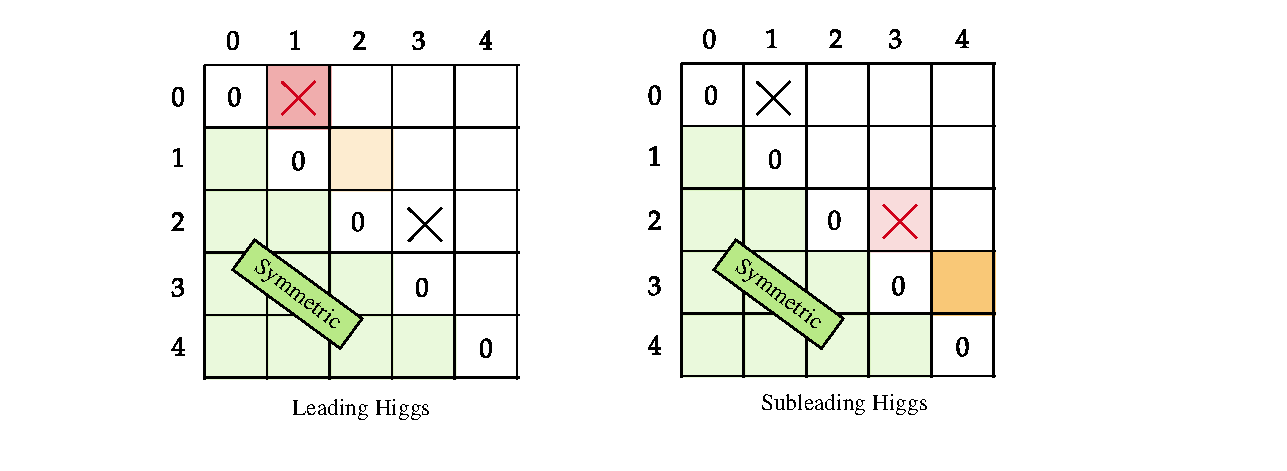
\includegraphics[width=0.8\linewidth]{Images/7.S:B/Prob diff/probability difference.pdf}
    \caption{Matrix of probabilities of the pairing of the jets. As 5 jets are considered for the pairing, we have a 5x5 matrix. The lines and the columns correspond to the jets used for the pairing. The jets of the columns correspond to the jets matched to one of the quarks coming from the decay of one Higgs and the lines to the other quark coming from the decay. In each square we will have the value of the probability of pairing these jets together. Since it is impossible to pair the same jet together, the diagonal is 0. This is a symmetric matrix as we can't distinguish quark from anti-quark in the detector. In red, we have the highest pairing probabilities that are compatible and in orange the second highest.}
    \label{fig: probabilities matrix}
\end{figure}

As we use 5 jets for the pairing, in Figure \ref{fig: probabilities matrix} a 5x5 matrix is shown. In each square we will have the value of the probability of matching these jets in the event together. Since it is impossible to pair the same jet together, the diagonal is 0. This is a symmetric matrix as we can't distinguish quark from anti-quark in the detector. 

To find the highest pairing probabilities, what SPANet does using this matrix is to first look for the overall highest probability, i.e the highest probability in the leading or sub-leading Higgs matrices. In Figure \ref{fig: probabilities matrix}, the overall highest probability is shown in dark red. Once this one has been found, we can move to the other matrix and find the highest probability that is compatible with the first one, i.e that is not sharing the same jets. The latter is showed in light red. (In this example, we see the matching is compatible since for the dark red the jets 0 and 1 are paired while for the light red the jets 3 and 2 are paired). As a next step to compute the PD variable is to find the second best pairing in this matrix. To do so, we will start by removing the best pairings determined earlier (red crosses) but we will also be removing the symmetric one in the other matrix (black crosses) as we have a symmetry between the leading and the sub-leading Higgs. Finally, we apply the same procedure to find the second best pairing. In this second example, the highest second pairing is depicted in dark orange. We find the complementary one on the other matrix in light orange.

To use this variable in the training, we will evaluate the best SPANet model presented in section \ref{subsection: Optimal config} on the signal and the background files that we will use to train the classifier. Once the evaluation is complete, we will add the PD variable found as global input to the classifier. 
In Figures \ref{fig: 2b data PD}, \ref{fig: 2b QCD PD} and \ref{fig: 4b QCD PD} we show the PD variable for signal and background events. We observe the high discriminant power of this variable, especially in Figures \ref{fig: 2b data PD} and \ref{fig: 2b QCD PD} when considering the 2b data and 2b QCD as background in our training.

\begin{figure}[hbt]
    \centering
    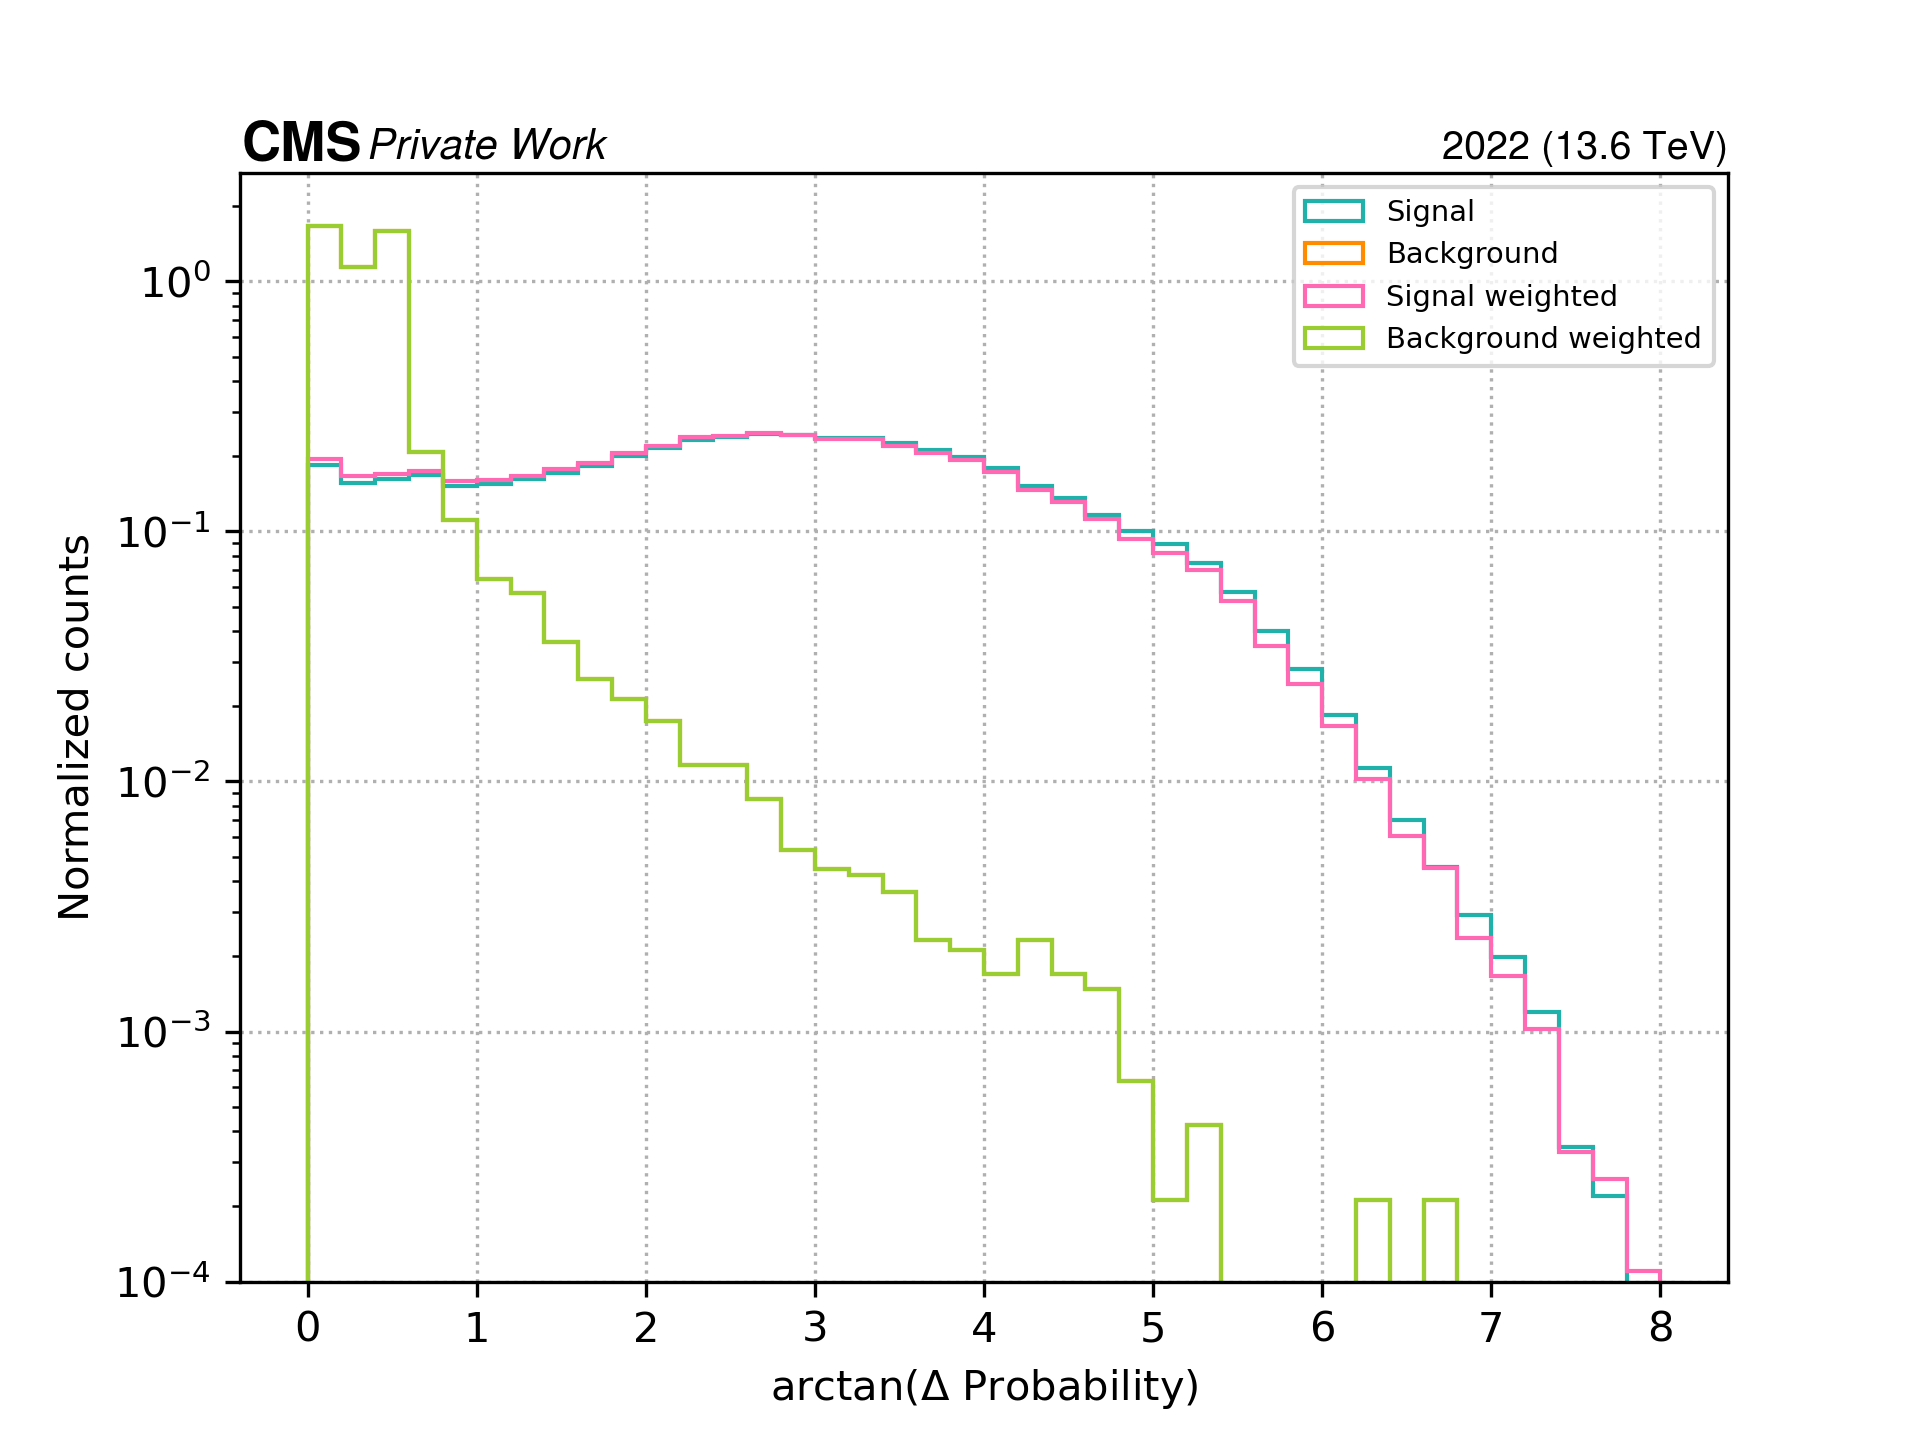
\includegraphics[width=0.7\linewidth]{Images/7.S:B/Prob diff/2b data reduced.png}
    \caption{Probability difference variable distribution in arc-tan for signal and 2b data background events. We show the weighted and non weighted events. As this is a 2b data sample, the weighted and non weighted distributions are the same due to the definition of Event weights}
    \label{fig: 2b data PD}
\end{figure}

\begin{figure}
    \centering
    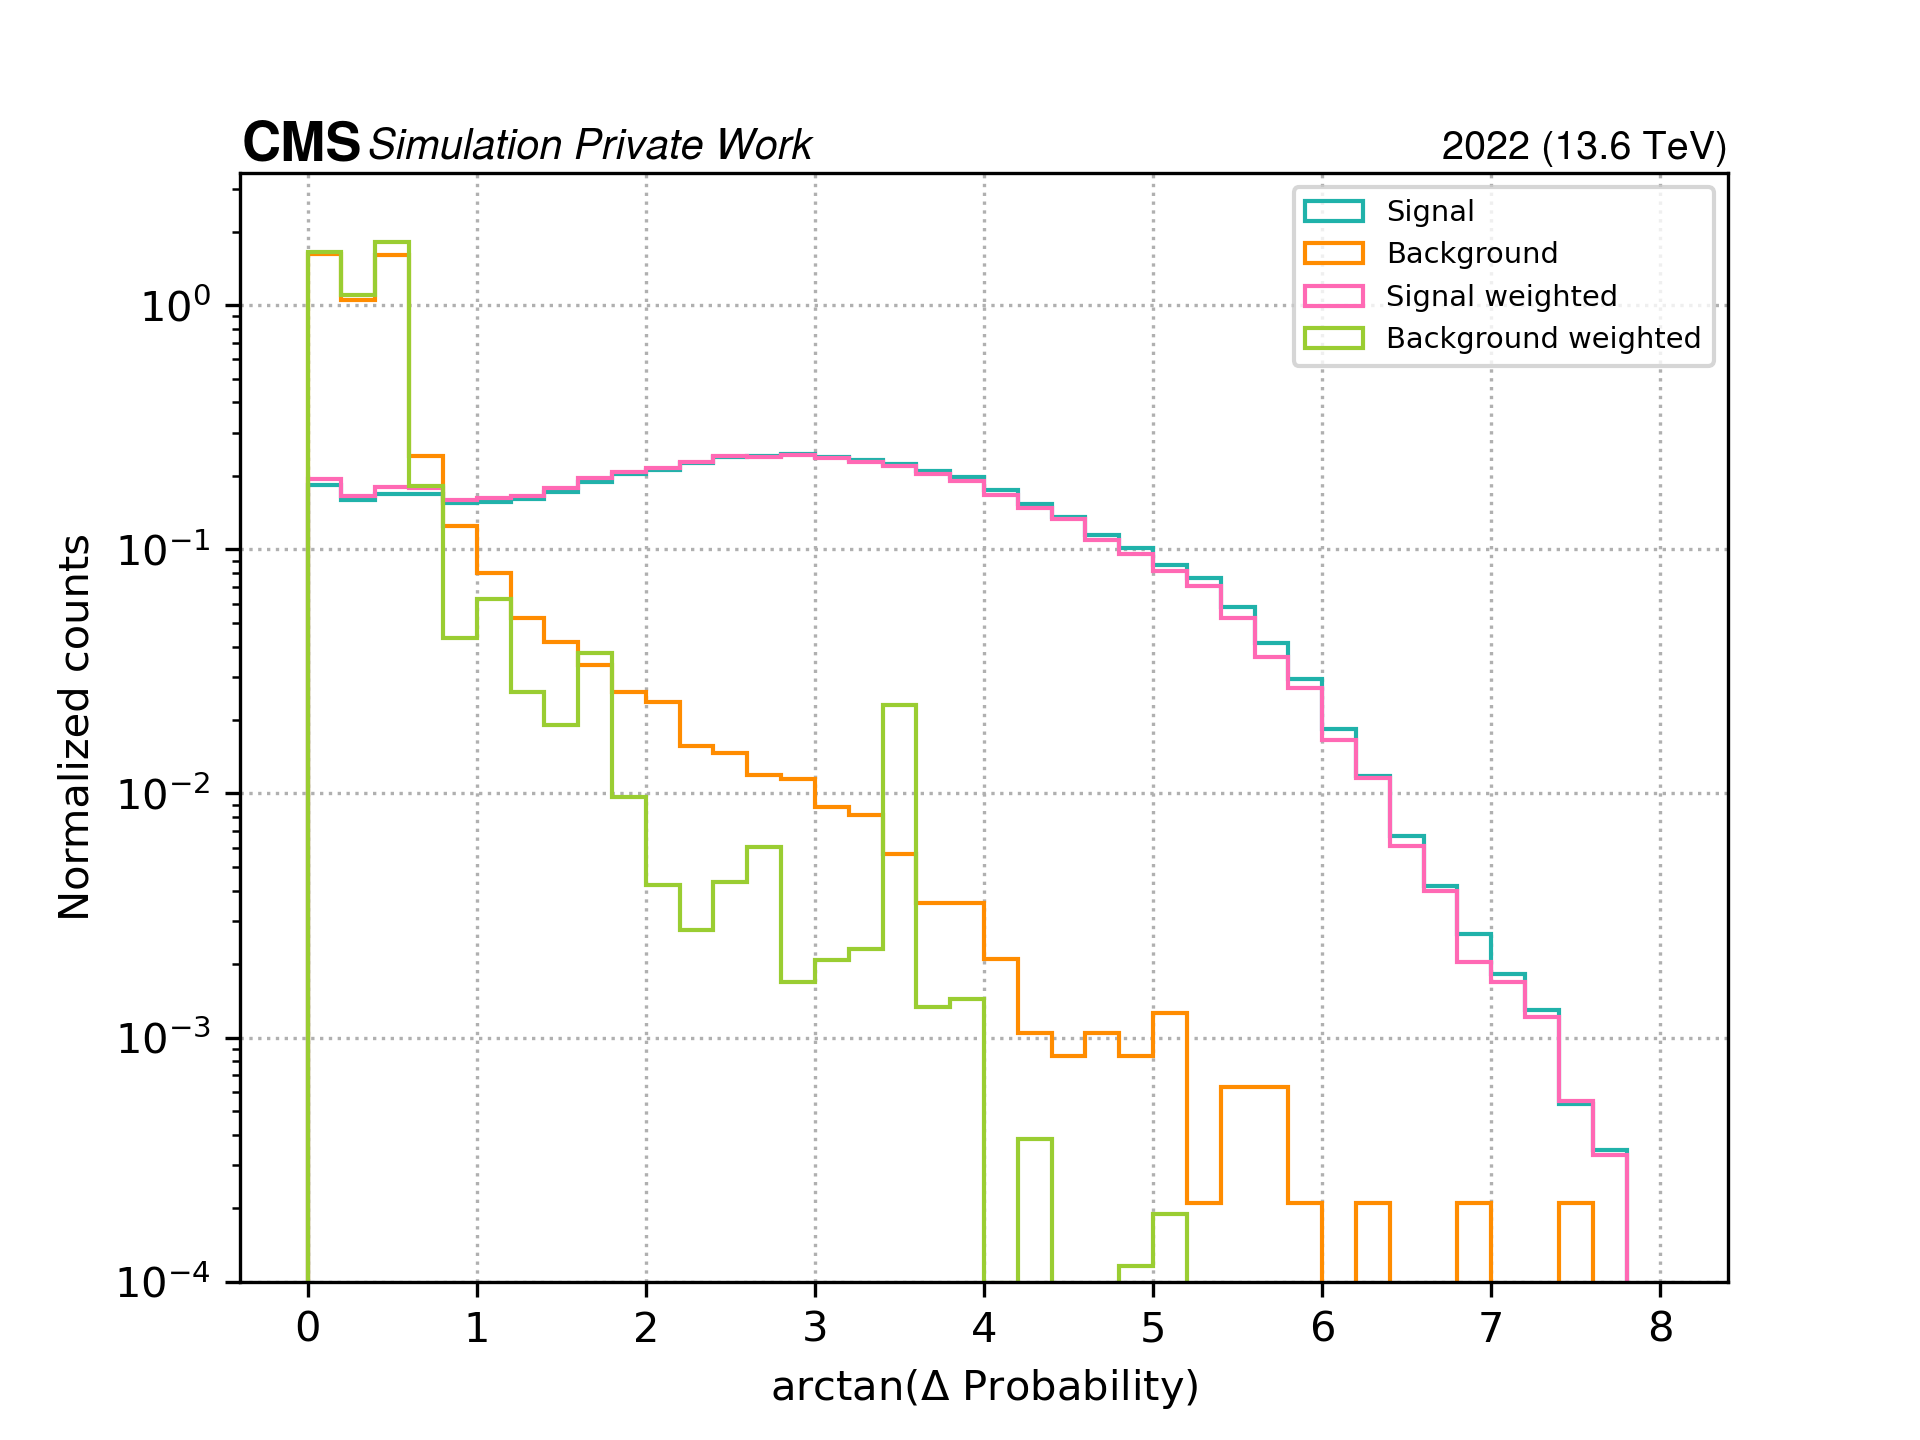
\includegraphics[width=0.7\linewidth]{Images/7.S:B/Prob diff/2b QCD arctan.png}
    \caption{Probability difference variable distribution in arc-tan for signal and 2b QCD background events. We show the weighted and non weighted events, using the Event weights.}
    \label{fig: 2b QCD PD}
\end{figure}


\begin{figure}[hbt]
    \centering
    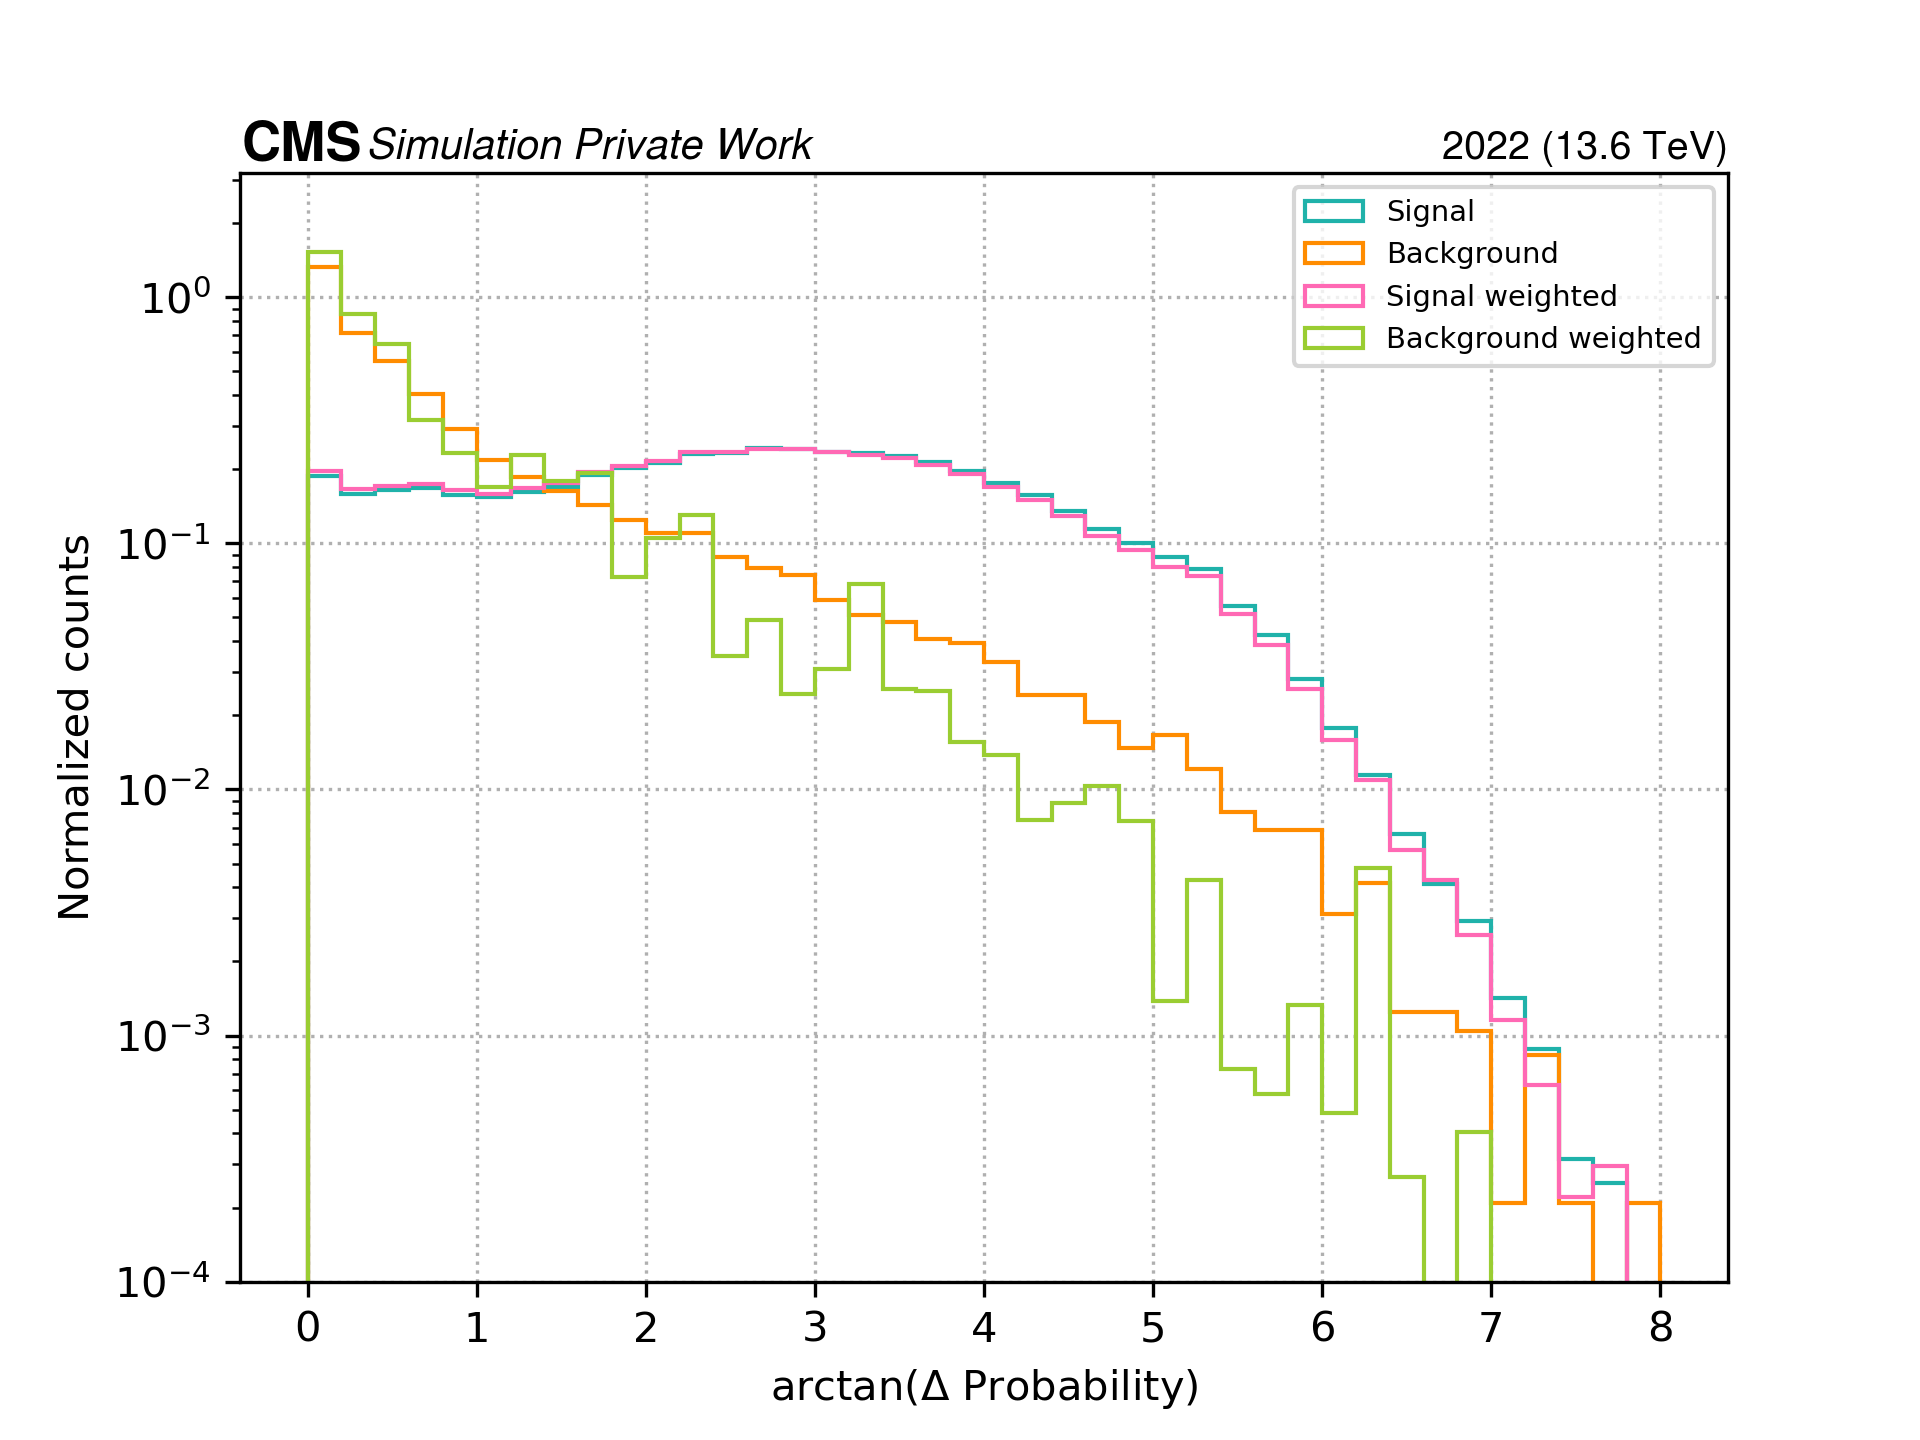
\includegraphics[width=0.7\linewidth]{Images/7.S:B/Prob diff/4b QCD arctan.png}
    \caption{Probability difference variable distribution in arc-tan for signal and 4b QCD background events. We show the weighted and non weighted events}
    \label{fig: 4b QCD PD}
\end{figure}

Finally, we show in Figure \ref{fig: ROC PD} the weighted ROCs of the probability difference distributions. We observe for 2b data and 2b QCD a sudden increase of FPR at 90\% of signal efficiency. This is due to the fact that most of the background events have a highest best pairing probability of around 0.5 and the second best one has a really a value close to 0, therefore we have a peak of events at $\Delta$Probability = 0.5, which corresponds to 90\% of signal efficiency and explains this excess in FPR events.

\begin{figure}
    \centering
    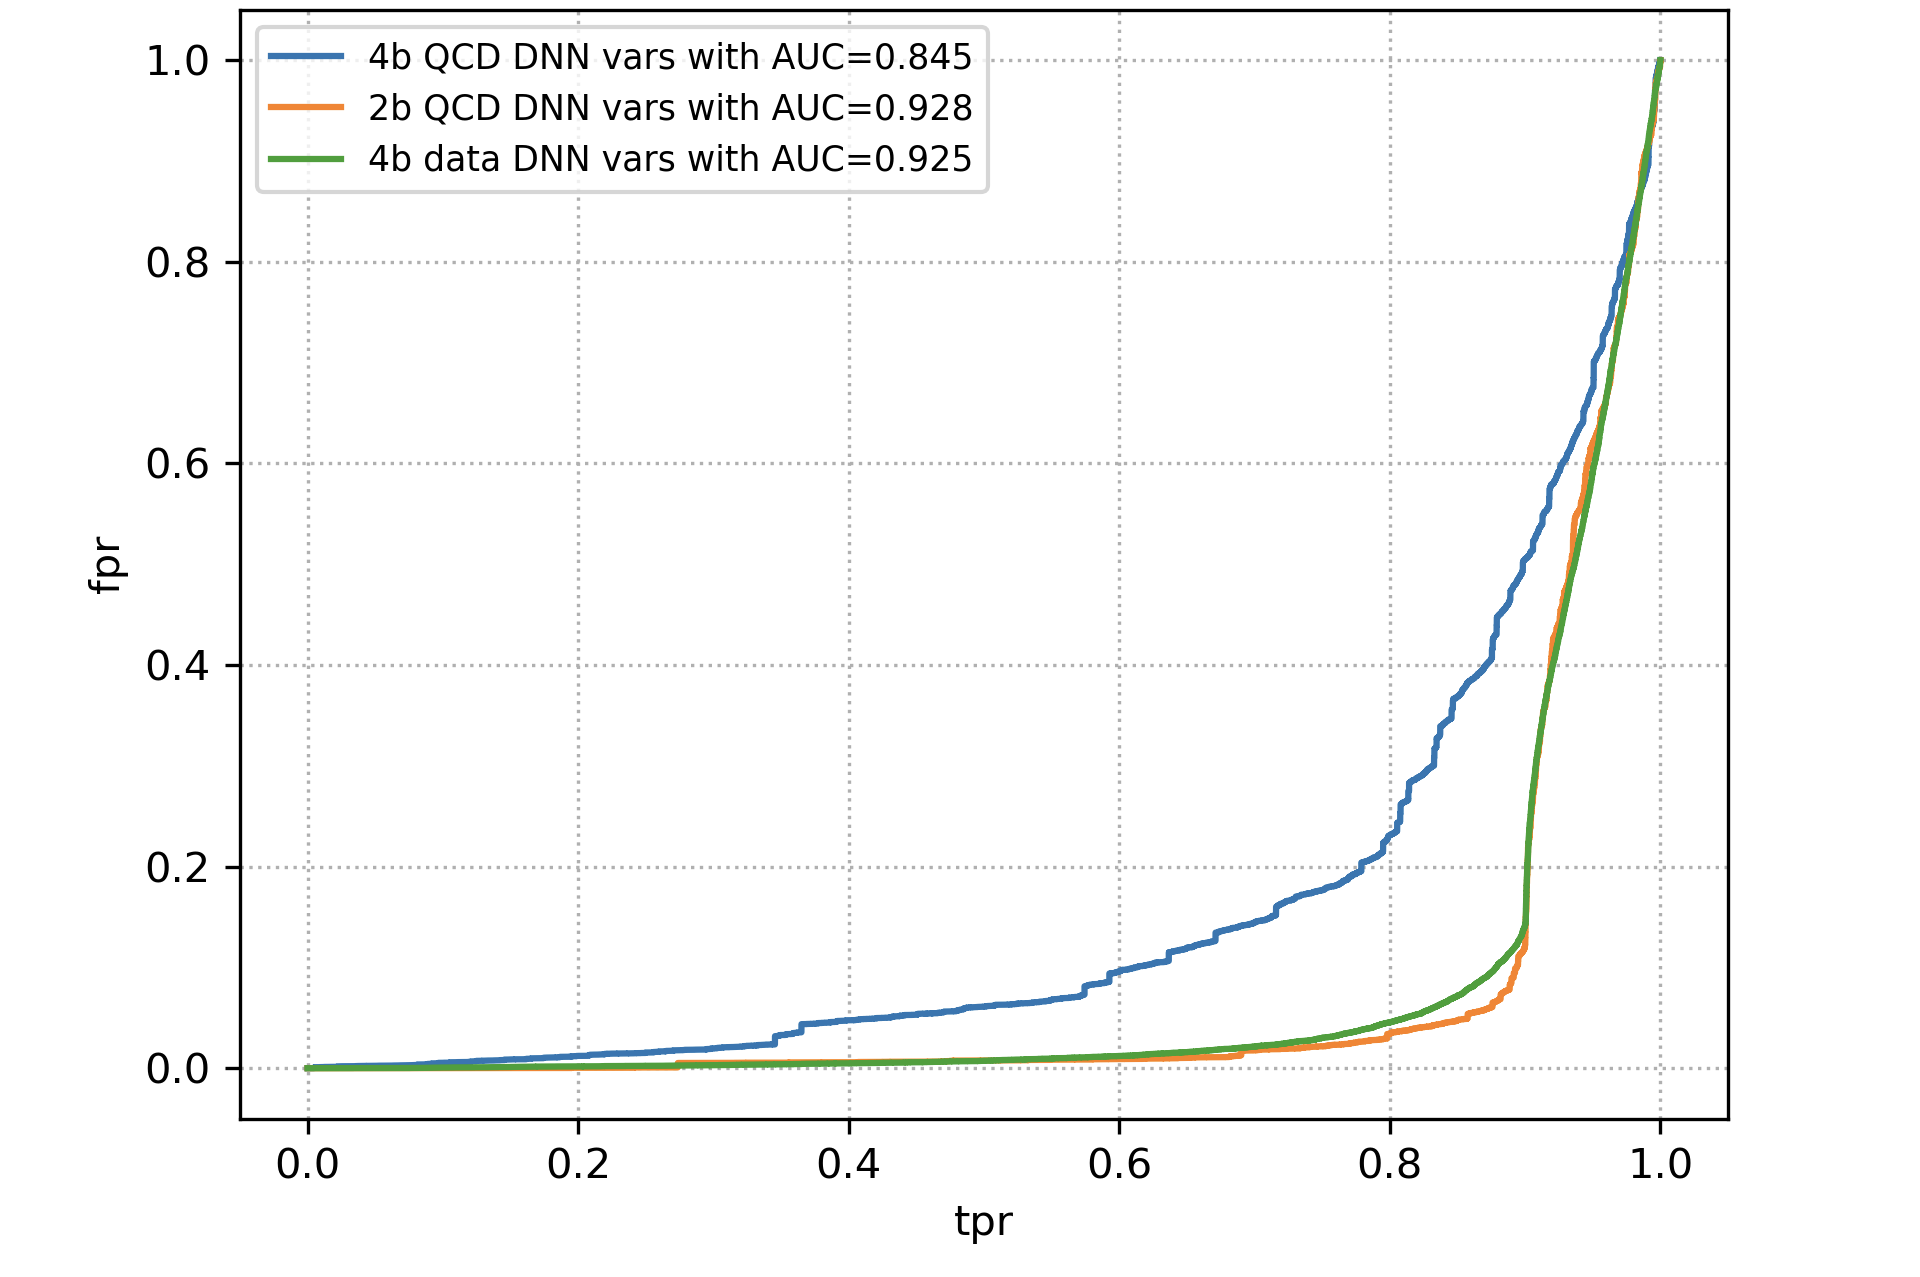
\includegraphics[width=0.7\linewidth]{Images/7.S:B/Prob diff/Probability difference ROC curve.png}
    \caption{Weighted ROCs of the probability difference variables distributions shown in Figures \ref{fig: 2b data PD}, \ref{fig: 2b QCD PD} and \ref{fig: 4b QCD PD} for 2b data, 2b QCD and 4b QCD}
    \label{fig: ROC PD}
\end{figure}

\clearpage

\subsection{Sample dependency} \label{subsection: sample dep}

As mentioned earlier, we would ideally like to use 4b morphed data for our training. Nevertheless, as this is not possible yet, we will test 3 different configurations for our training. For each configuration we will be comparing the training using only DNN variables as inputs or DNN and Probability difference variables. These configurations are summarized in Table \ref{table: S/B trainings}.

\begin{table}[h!]
\centering
\begin{tabular}{|M{3cm}|M{10cm}|}
 \hline
 Configuration  & Inputs  \\
 \hline
 \multirow{2}{*}[0pt]{\raisebox{-3.4\height}{4b QCD}}  & \begin{itemize}[itemsep=0.01em]
    \item 4-vector of the 5 jets in leading b-tag
    \item DNN variables (global input)
 \end{itemize} \\ 
 \cline{2-2}
   &  \begin{itemize}[itemsep=0.01em]
    \item 4-vector of the 5 jets in leading b-tag
    \item DNN and PD variables (global input)
 \end{itemize} \\
 \hline
 \multirow{2}{*}[0pt]{\raisebox{-3.4\height}{2b QCD}}  & \begin{itemize}[itemsep=0.01em]
    \item 4-vector of the 5 jets in leading b-tag
    \item DNN variables (global input)
 \end{itemize} \\ 
 \cline{2-2}
   &  \begin{itemize}[itemsep=0.01em]
    \item 4-vector of the 5 jets in leading b-tag
    \item DNN and PD variables (global input)
 \end{itemize} \\
 \hline
  \multirow{2}{*}[0pt]{\raisebox{-3.4\height}{2b data}}  & \begin{itemize}[itemsep=0.01em]
    \item 4-vector of the 5 jets in leading b-tag
    \item DNN variables (global input)
 \end{itemize} \\ 
 \cline{2-2}
   &  \begin{itemize}[itemsep=0.01em]
    \item 4-vector of the 5 jets in leading b-tag
    \item DNN and PD variables (global input)
 \end{itemize} \\
 \hline
\end{tabular}
\caption{Configuration of the different trainings for S/B classification. We will be comparing the different configurations as well as the inputs for each configuration}
\label{table: S/B trainings}
\end{table}

So as to have a better comparison to the performance of the DNN used in Run 2 presented in the AN (cite) where they used the 4b morphed data, we will extrapolate our results to have an idea what we would obtain if we used 4b data in our training. To do so, we will extrapolate the value of the area under the curve (AUC) by using the following expression:

\begin{equation}
    \text{AUC}(\text{4b-data})= \text{AUC}(\text{2b-data}_f) \times \textcolor{BlueGreen}{\frac{\text{AUC}(\text{4b-QCD})}{\text{AUC}(\text{2b-QCD}_r)}} \times \textcolor{WildStrawberry}{\frac{\text{AUC}(\text{2b-QCD}_r)}{\text{AUC}(\text{2b-data}_r)}}
    \label{eq: extrapolation}
\end{equation} 
\noindent Since the 4b morphed data and the 2b data have the same number of events, we use the value of the AUC of the full statistics 2b data (black). In order to go from 2b to 4b data, we would like to take into account the b-tag dependency of our model. This value will be given by the first ratio (\textcolor{BlueGreen}{blue}). Nevertheless, this b-tag ratio is computed using QCD MC samples, therefore we need to take into account the difference that the model (meaning using either QCD or data samples) makes. This model dependency is given by the second ratio (\textcolor{WildStrawberry}{pink}).  Finally, on both ratios we see $r$, that stands for reduced statistics. As we aim to probe the b-tag dependency and the model dependency, we perform a random removal of events so that the effective statistics are the same. In this case, we will use the statistics of the 4b data ($\sim$ 100k events), since it is the dataset with the lowest number of events.

For the extrapolation of the ROC curve we will use Eq.(\ref{eq: extrapolation})  to compute the value of the false positive rate (FPR) instead of the AUC. Nonetheless, we will apply this formula to the true positive rate (TPR) values or this will result in a rescaling of thee 2b-data ROC. This is why, for the 4b-data extrapolated ROC we will be using the modified FPR values and the TPR values from the 2b-data full statistics training. 

Our ultimate goal will then be to perform this extrapolation. However, we first need the results of the trainings with 4b-QCD, 2b-QCD reduced statistics, 2b-data reduced statistics and 2b-data full statistics that will be presented in the following sections.


\subsection{Results on the input comparison} \label{subsection: results on the trainings}

%Compare weighted and non weighted
%also for the SPANet

In this section we will present the results of the trainings shown in Table \ref{table: S/B trainings}. In Figures \ref{fig: 4b QCD comp input}, \ref{fig: 2b QCD comp input} and \ref{fig: 2b data comp input} we show the weighted ROCs of these trainings. From these figures one can see that for 2b-QCD (Fig.\ref{fig: 2b QCD comp input}) and 2b-data (Fig.\ref{fig: 2b data comp input}) samples, adding the PD variable results in a significant improvement of our classification. For the 4b-QCD configuration (Fig. \ref{fig: 4b QCD comp input})  the performance is only slightly increased.  The difference in the improvement when adding the PD variable between 4b and 2b can be understood by looking at Figures \ref{fig: 2b data PD}, , \ref{fig: 2b QCD PD} and \ref{fig: 4b QCD PD}. Indeed, we observe that the discriminant power of the PD variable is lower when using 4b-QCD.

Nevertheless, it is important to point out that we performed several trainings with the 4b configuration and it occurred that we obtained a worse performance when adding the PD. This observed feature is very surprising and to try to understand it, in the following section, we will be interested in assessing the variability of these trainings with respect to the ROCs.

\begin{figure}[hbt]
    \centering
    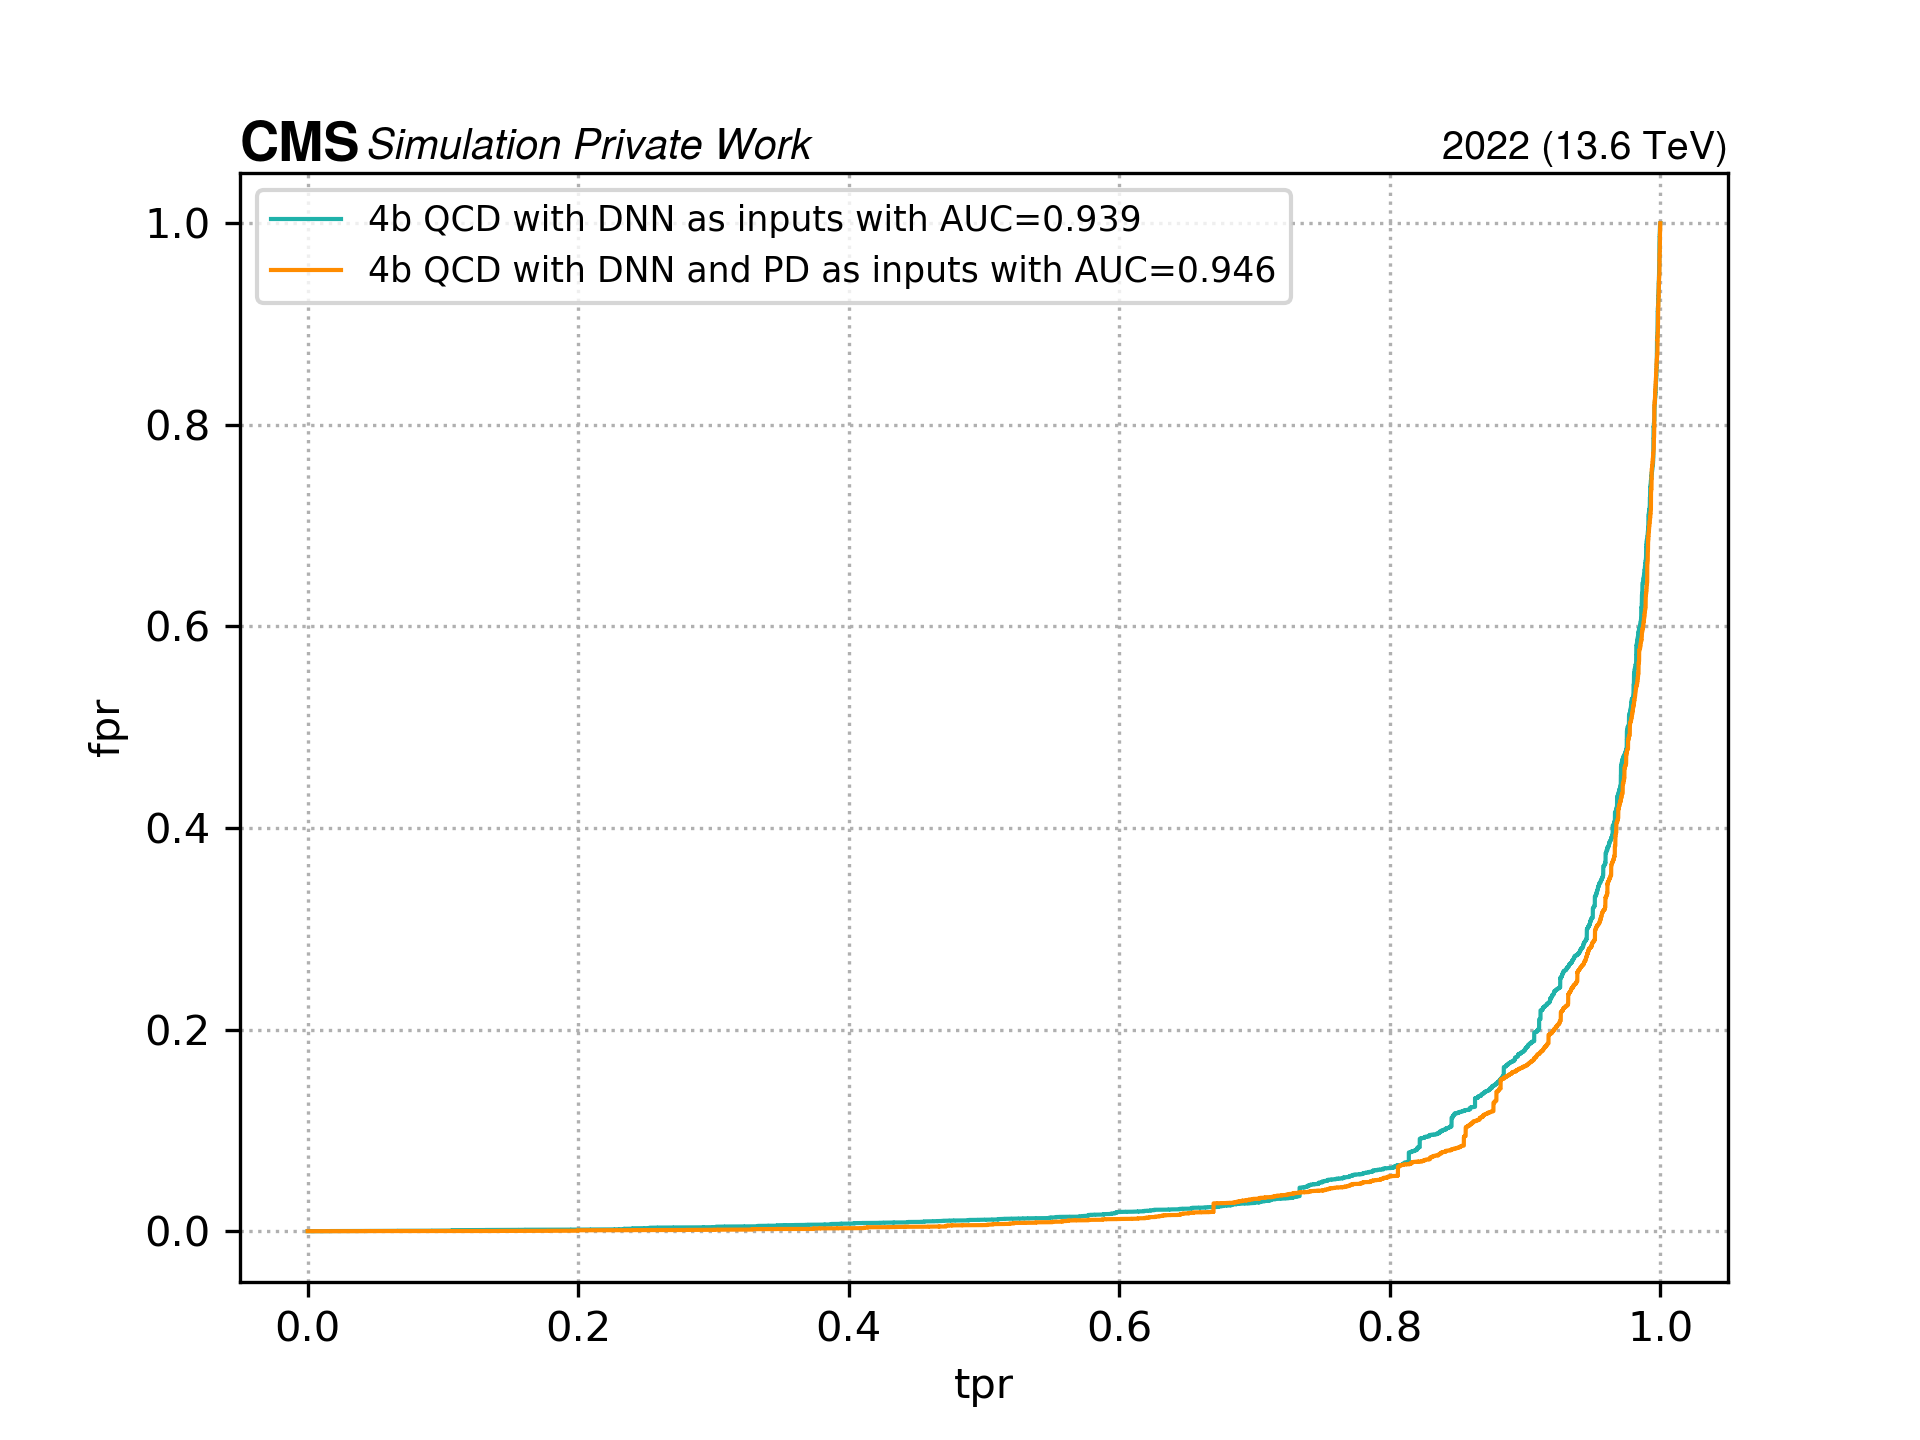
\includegraphics[width=0.7\linewidth]{Images/7.S:B/Inputs/4b QCD bis.png}
    \caption{Weighted ROCs comparing the performance using different global inputs for the 4b-QCD configuration presented in Table \ref{table: S/B trainings}}
    \label{fig: 4b QCD comp input}
\end{figure}

\begin{figure}[hbt]
    \centering
    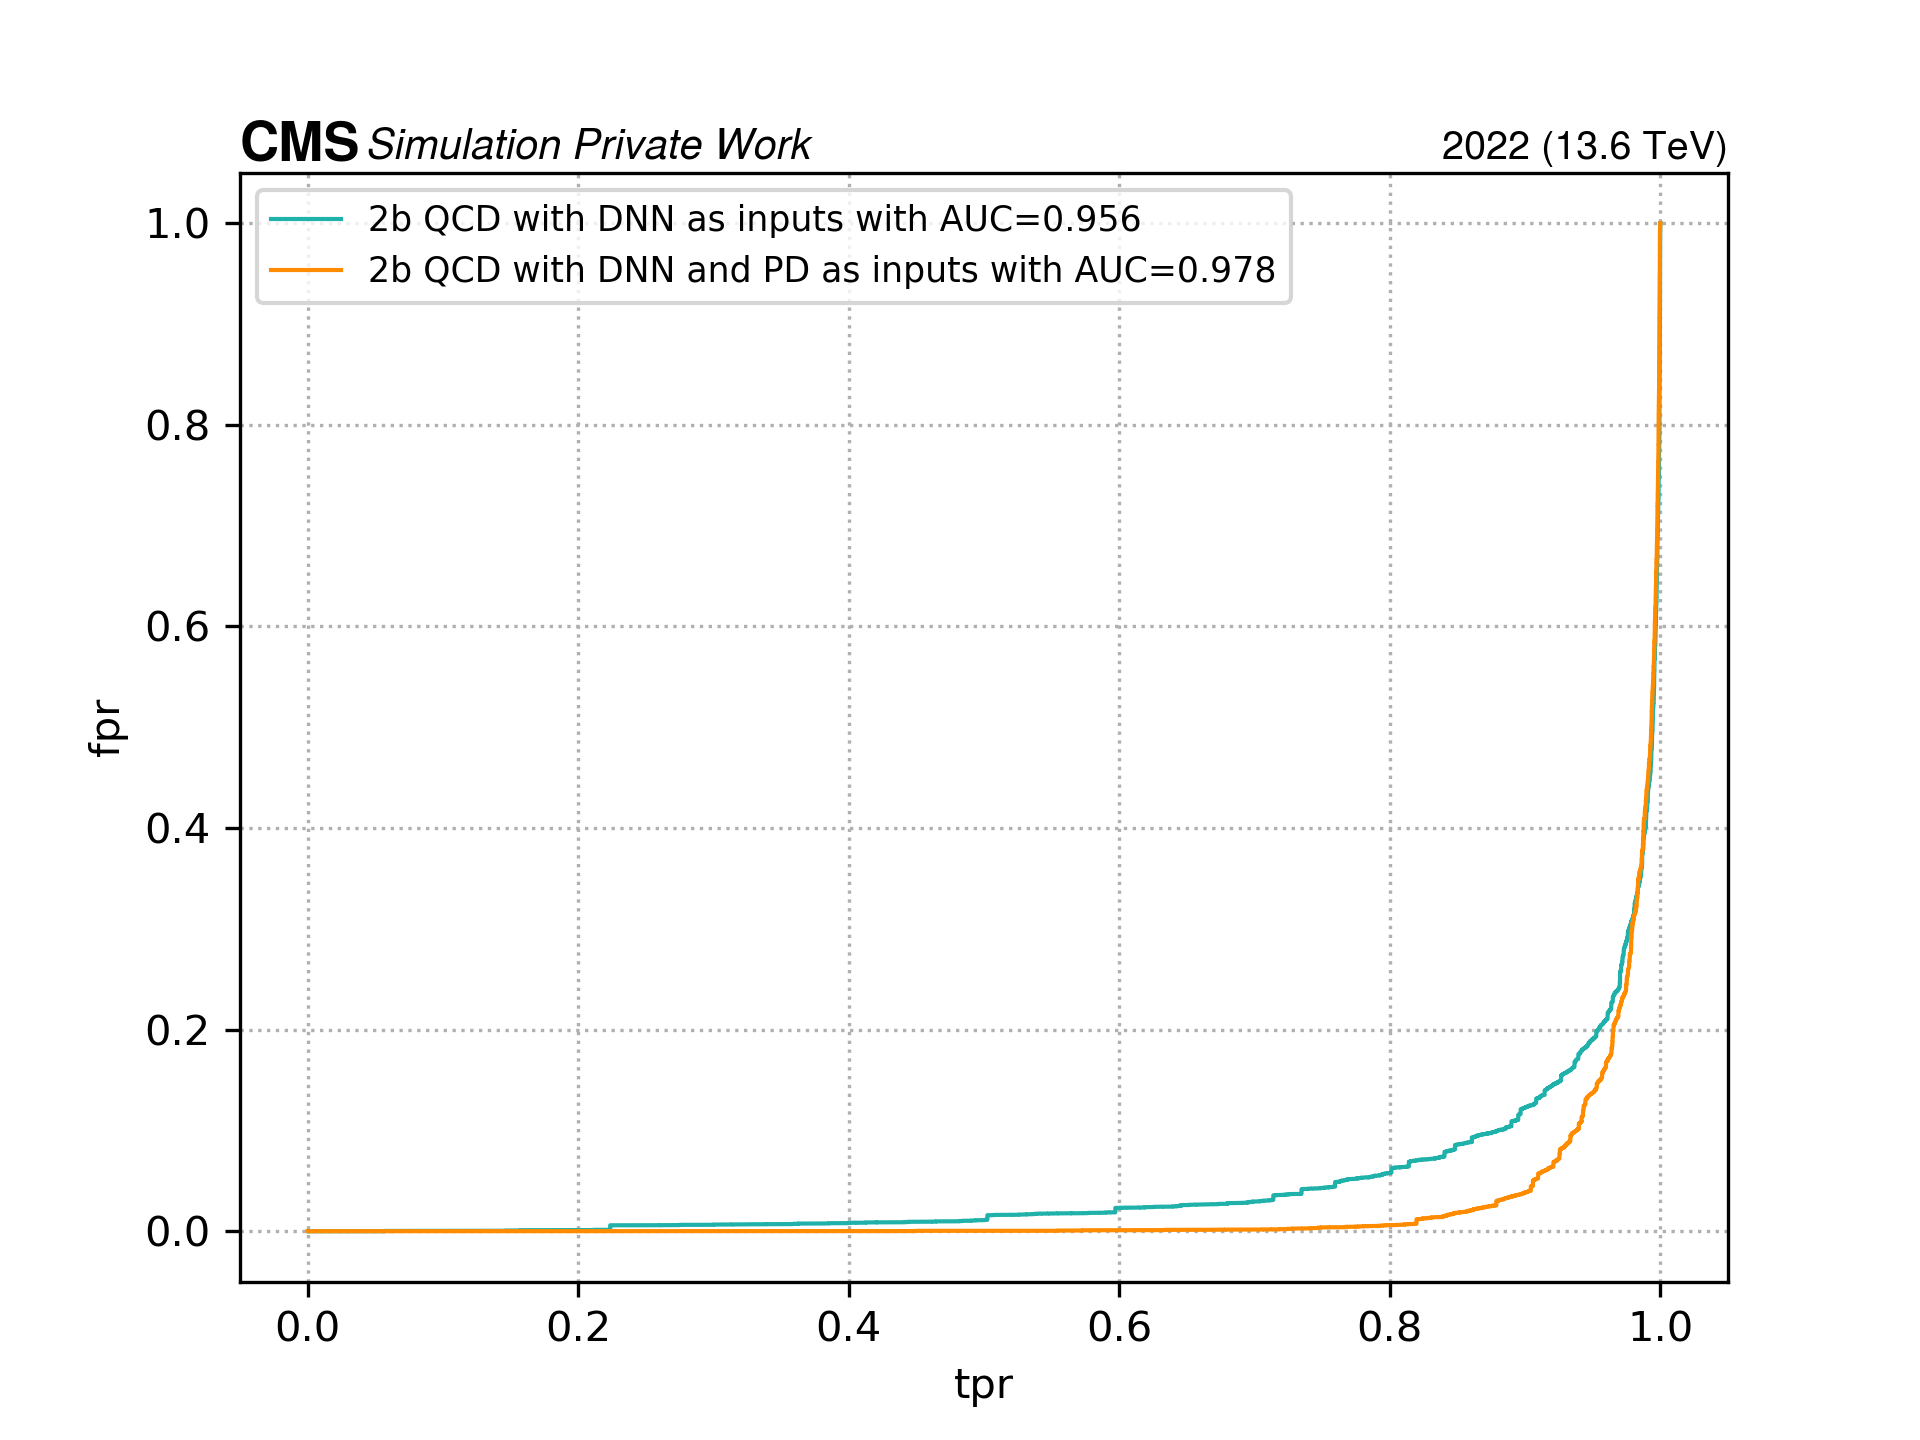
\includegraphics[width=0.7\linewidth]{Images/7.S:B/Inputs/2b QCD.png}
    \caption{Weighted ROCs comparing the performance using different global inputs for the 2b-QCD configuration presented in Table \ref{table: S/B trainings}}
    \label{fig: 2b QCD comp input}
\end{figure}

\begin{figure}[hbt]
    \centering
    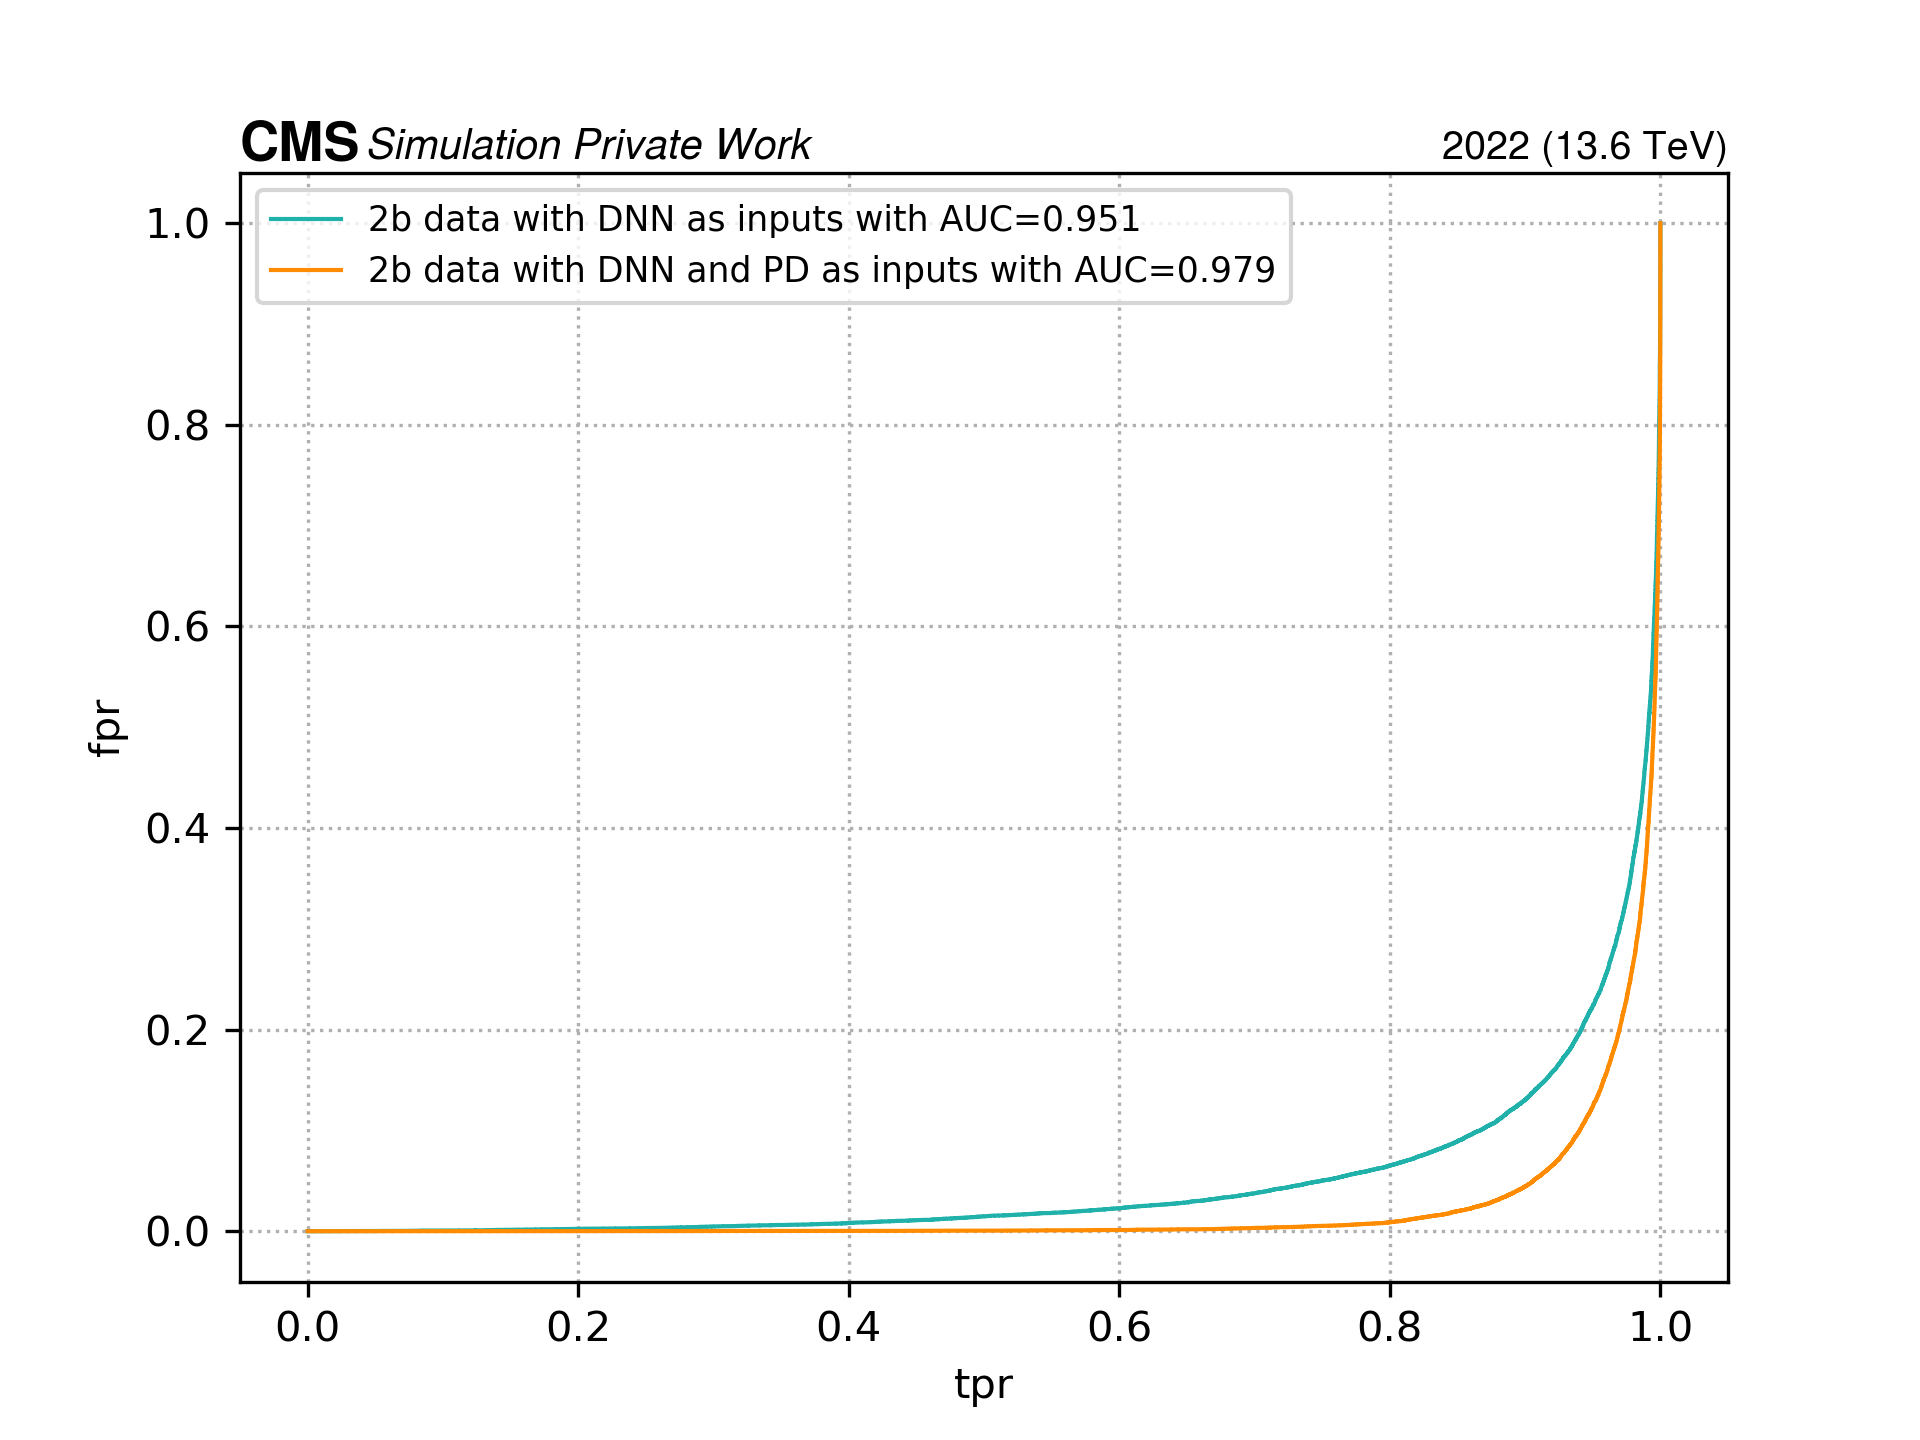
\includegraphics[width=0.7\linewidth]{Images/7.S:B/Inputs/2b data.png}
    \caption{Weighted ROCs comparing the performance using different global inputs for the 2b-data configuration presented in Table \ref{table: S/B trainings}}
    \label{fig: 2b data comp input}
\end{figure}

Finally, we show the non weighted ROC for the 4b-QCD configuration. We observe in Figure \ref{fig: 4b QCD ROC no weights} that the distribution is much smoother compared to the one in Figure \ref{fig: 4b QCD comp input}. This feature can be understood by looking at the SPANet output of the classification, in Figure \ref{fig: SPANet output S/B 4b QCD}. Indeed adding the weights adds a lot of fluctuation to the distribution which are then reflected in the ROC. Nevertheless, in the following we will only show the weighted ROC curves as they allow a correct comparison to the AN results.

\begin{figure}[hbt]
    \centering
    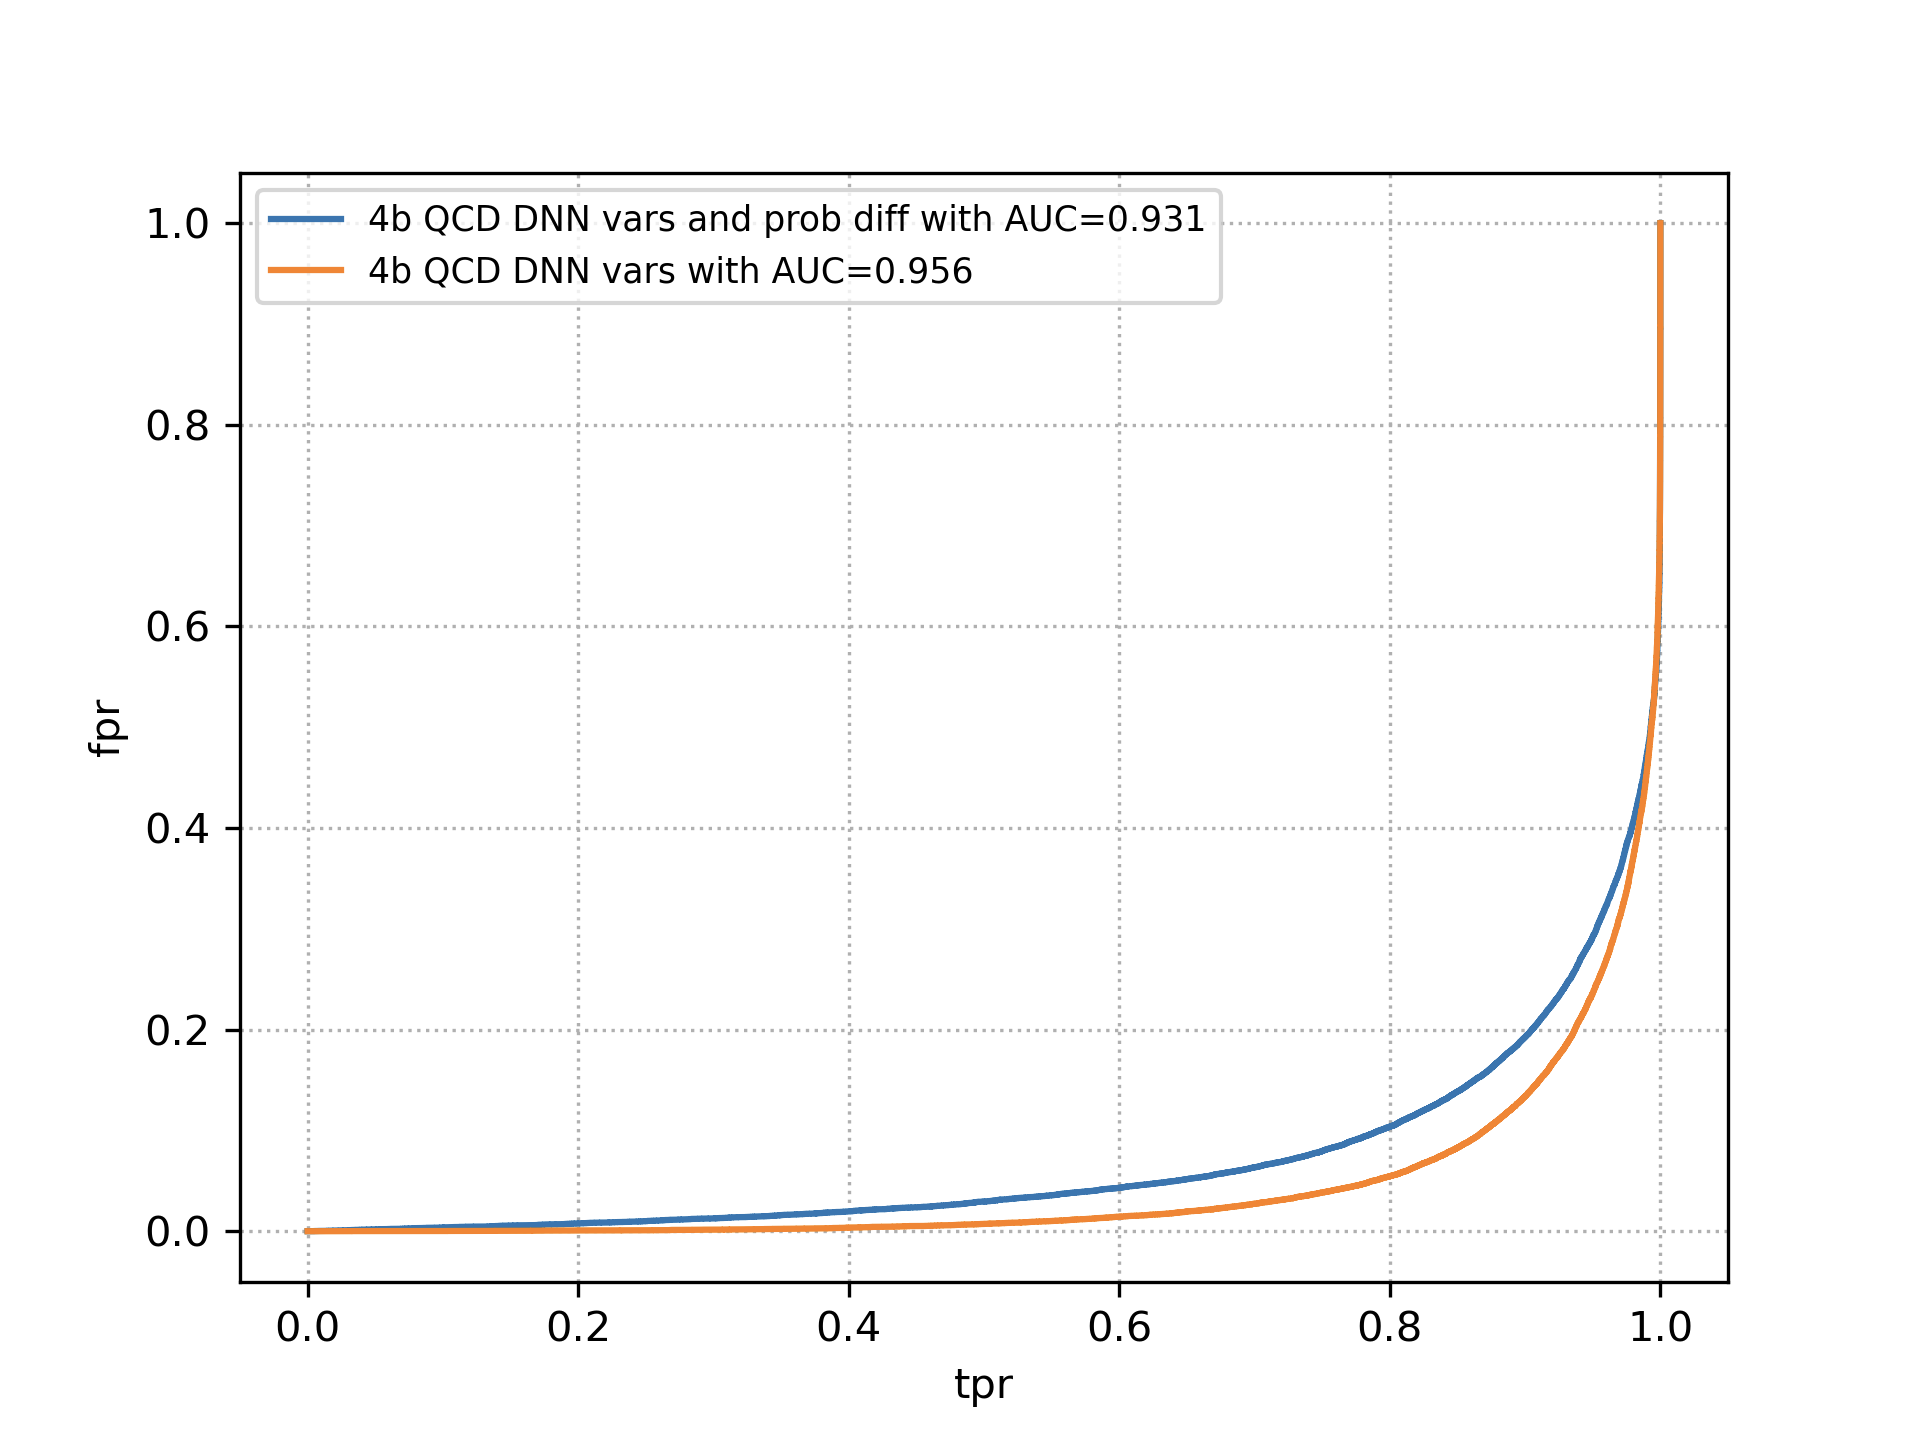
\includegraphics[width=0.7\linewidth]{Images/7.S_B/Inputs/no weights 4b QCD.png}
    \caption{Unweighted ROCs comparing the performance using different global inputs for the 4b-QCD configuration presented in Table \ref{table: S/B trainings}}
    \label{fig: 4b QCD ROC no weights}
\end{figure}

\begin{figure}
    \centering
    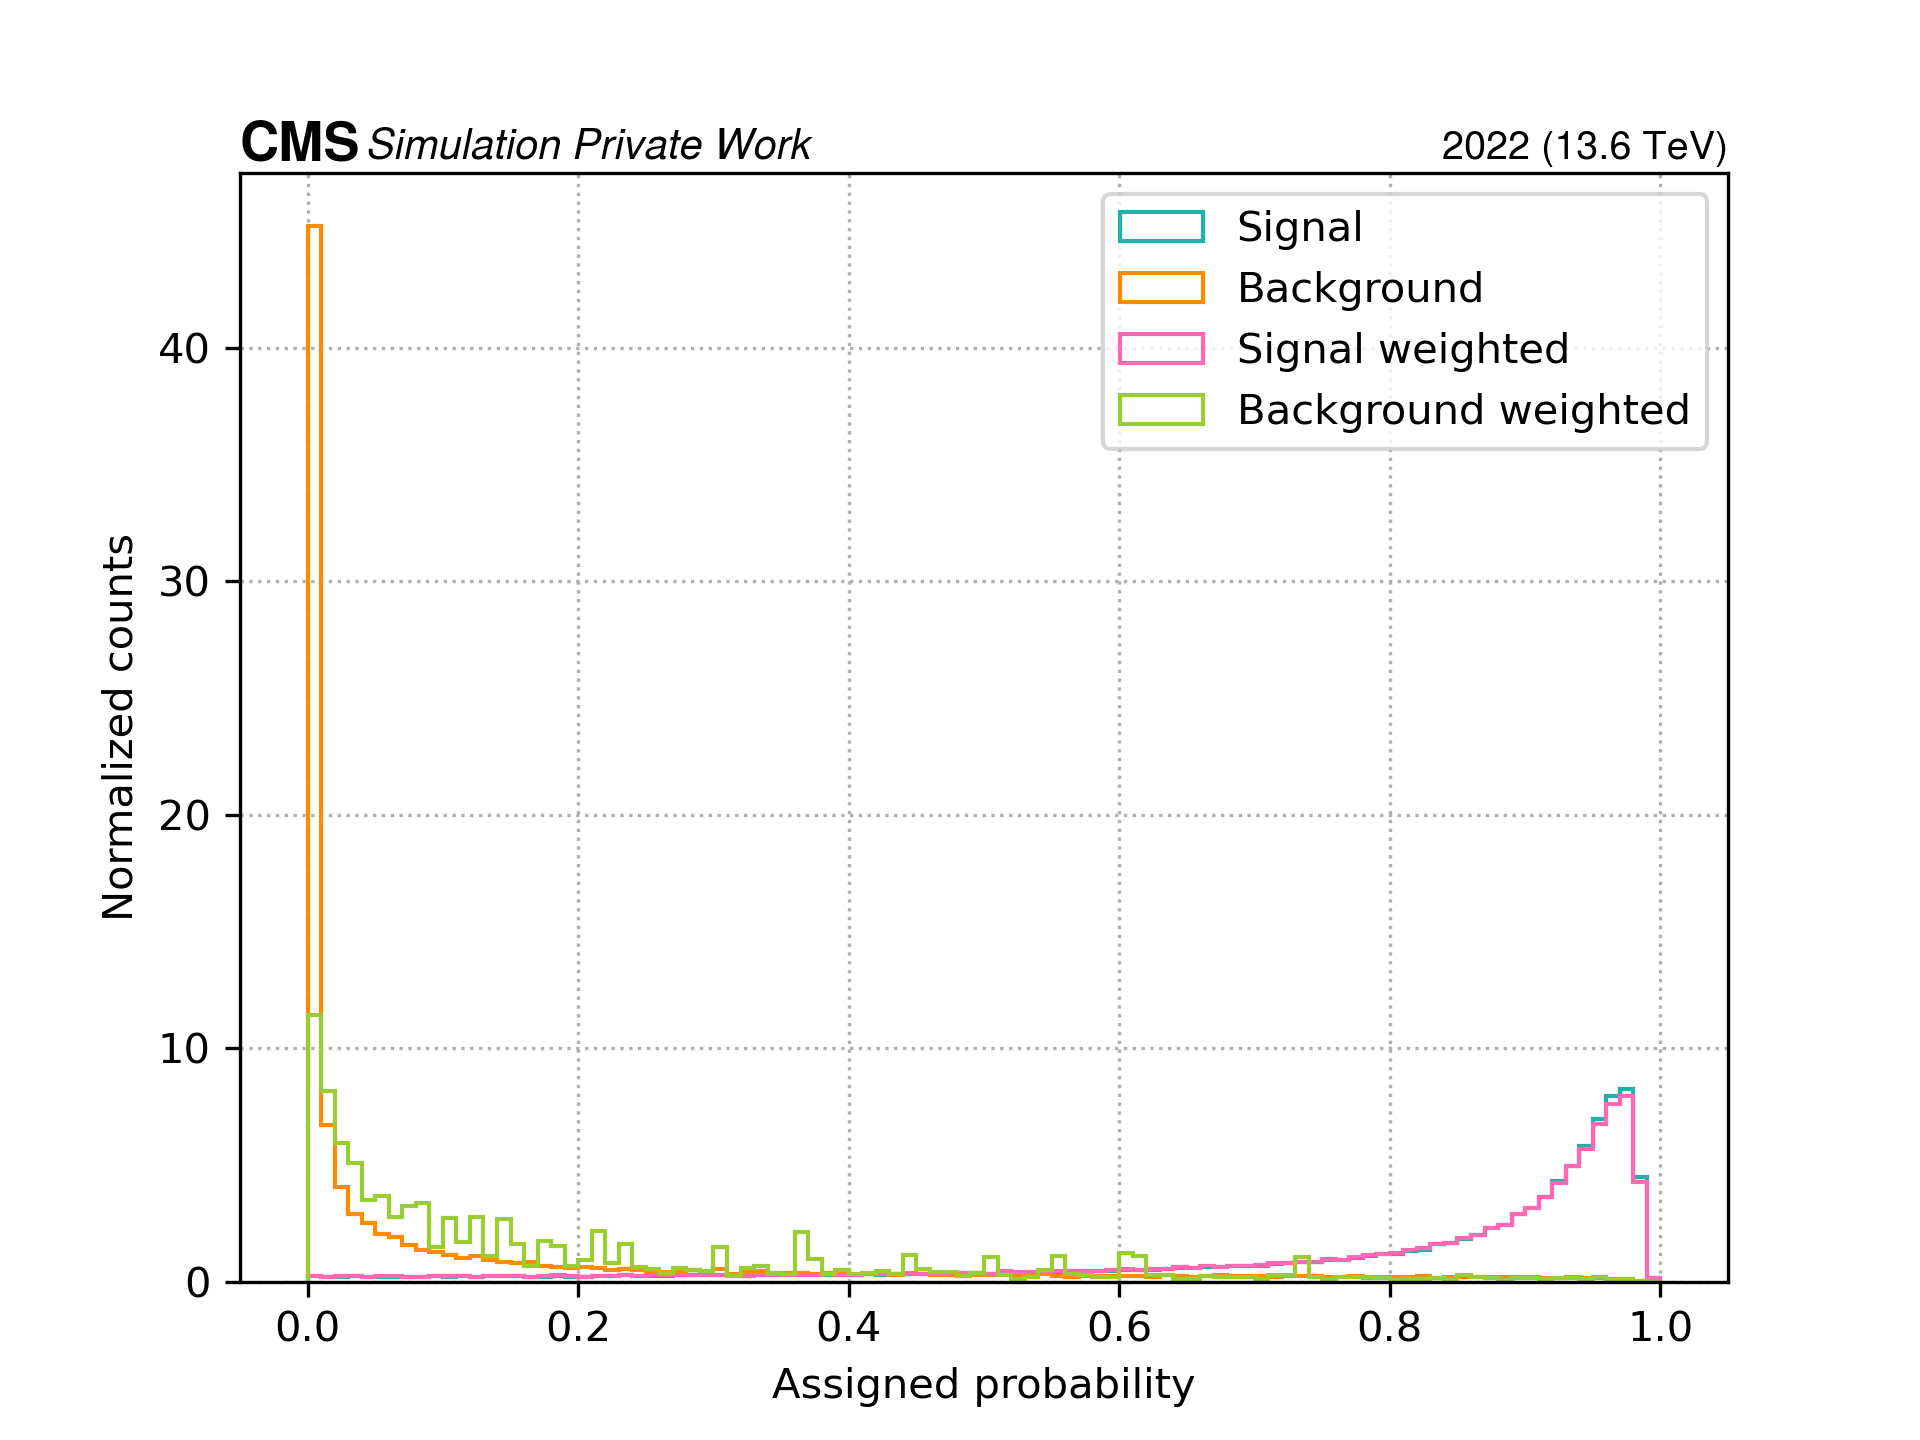
\includegraphics[width=0.7\linewidth]{Images/7.S:B/Classification outputs/4b QCD dnn.png}
    \caption{SPANet output for the classification training using the 4b QCD configuration and DNN as input variables. It shows the probability assigned to the signal events and the probability assigned to the background events by our network. We can see the difference in the distribution when applying the weights}
    \label{fig: SPANet output S/B 4b QCD}
\end{figure}

\clearpage

\subsection{Assessing the variability of the trainings} \label{subsection: var of training S/B}

Unlike in section \ref{subsection: pairing variability}, here we look to asses the variability of the performance seen in the ROCs instead of in the validation accuracy. Nonetheless, as was done in section \ref{subsection: pairing variability}, we performed different trainings using the same configuration but fixing the seed to randomly initialize the weights. In Figures \ref{fig: 4b QCD v ariability}, \ref{fig: 2b QCD v ariability}, \ref{fig: 2b data v ariability} we can see the results of these trainings. A summary of the AUC values seen in these figures can be found in Table \ref{table: Spread of the trainings}. From looking at these values, one finds that the variability using 2b-QCD and 2b-data configurations is acceptable, as it is for 4b-QCD using DNN variables as inputs. Nevertheless, for 4b-QCD using DNN and PD as inputs we find a large uncertainty. This wide variability seen in Figure \ref{fig: 4b QCD DNN PD}, can then explain the surprising results we pointed out in section \ref{subsection: results on the trainings}. Therefore we can't state that our performance using 4b-QCD with DNN and PD improves our performance with respect to only DNN variables. We can conclude that they are the same within the variability. 

% ases tghe variability by looking at the AUCs (before: first thing)

\begin{figure}[hbt]
\centering
\begin{subfigure}{.5\textwidth}
  \centering
  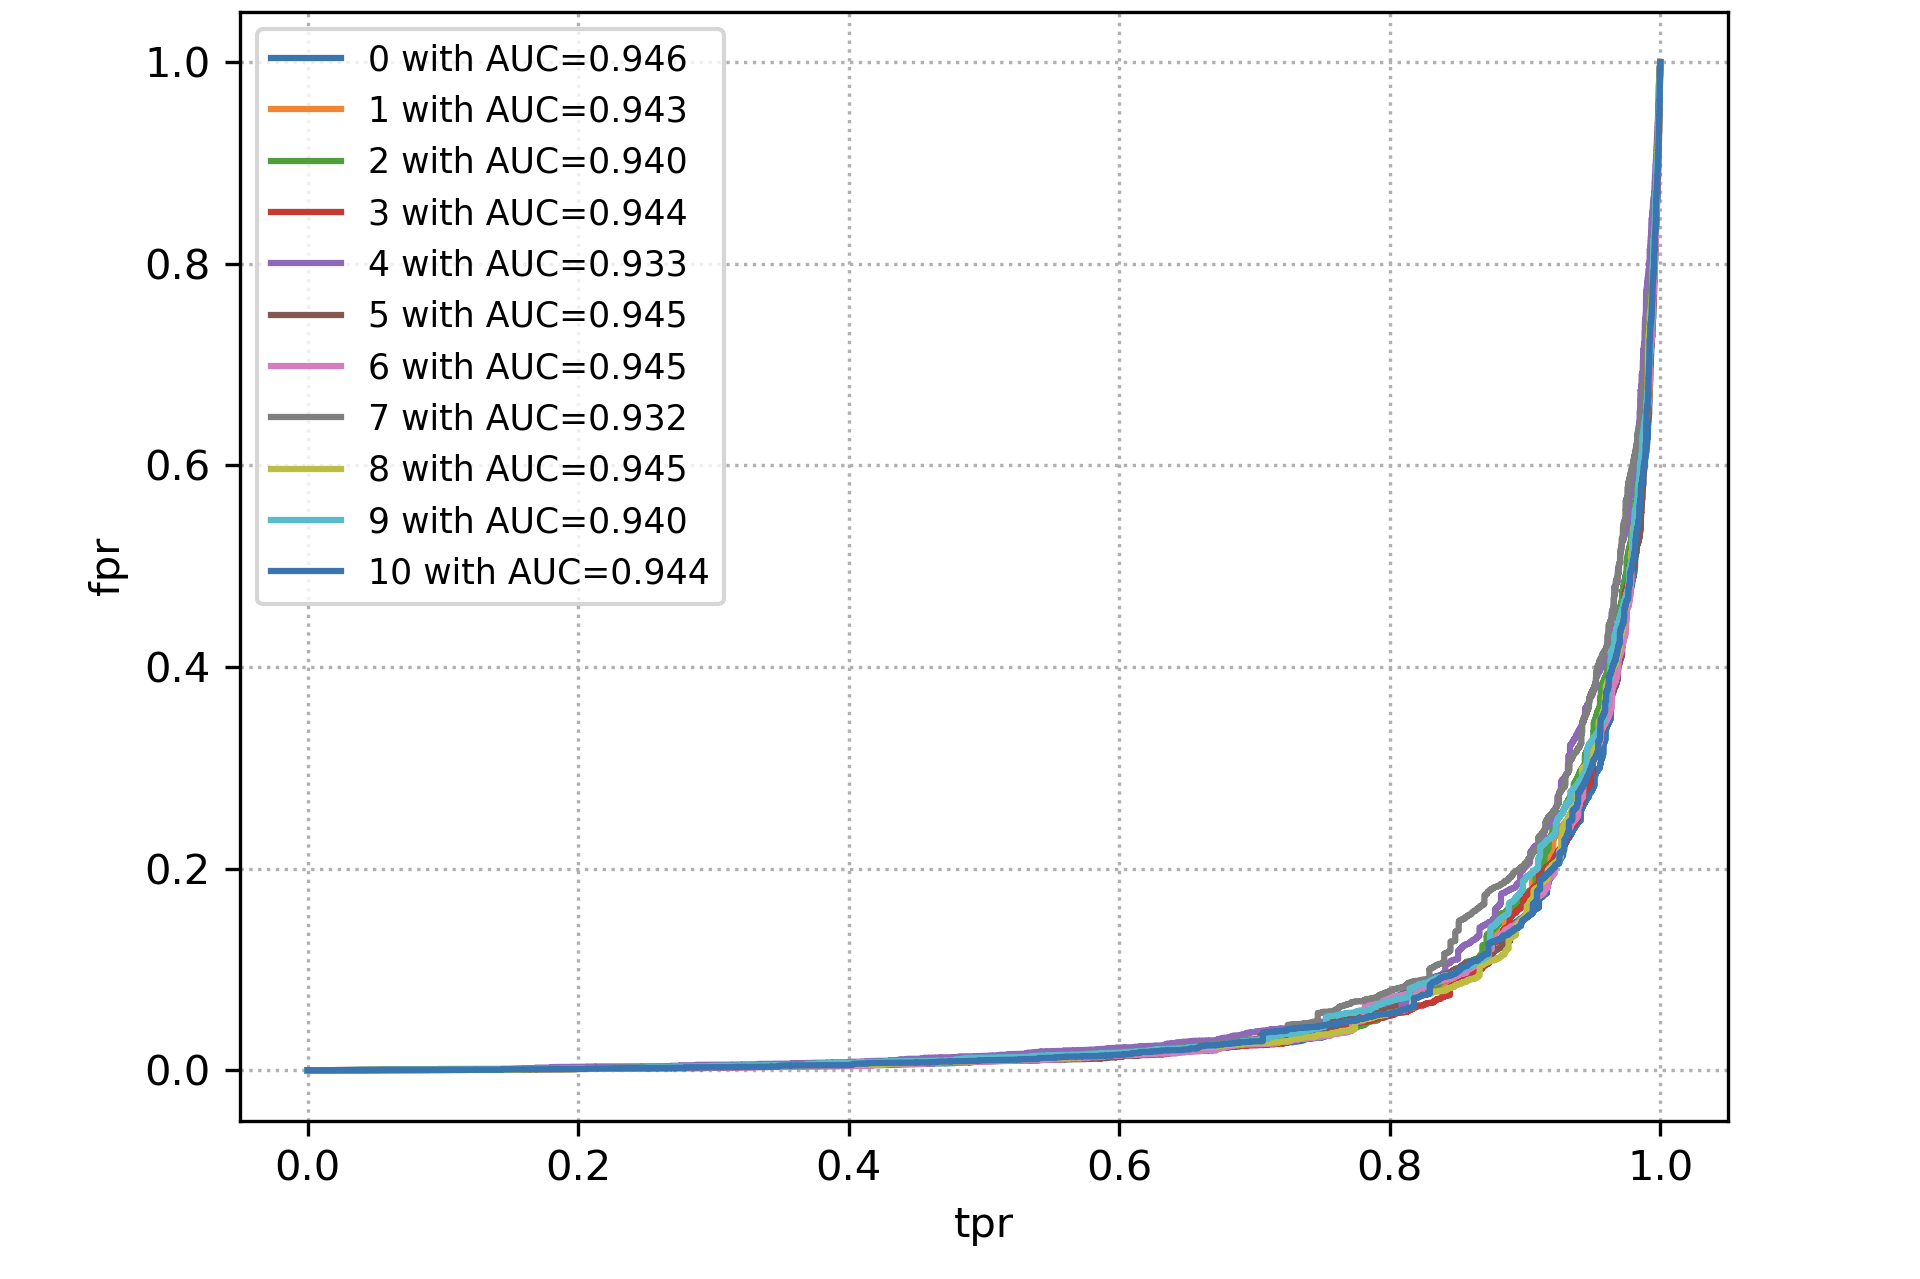
\includegraphics[width=1.1\linewidth]{Images/7.S_B/Variability/4b QCD DNN.png}
  \caption{DNN as global input}
  \label{fig: 4b QCD DNN}
\end{subfigure}%
\begin{subfigure}{.5\textwidth}
  \centering
  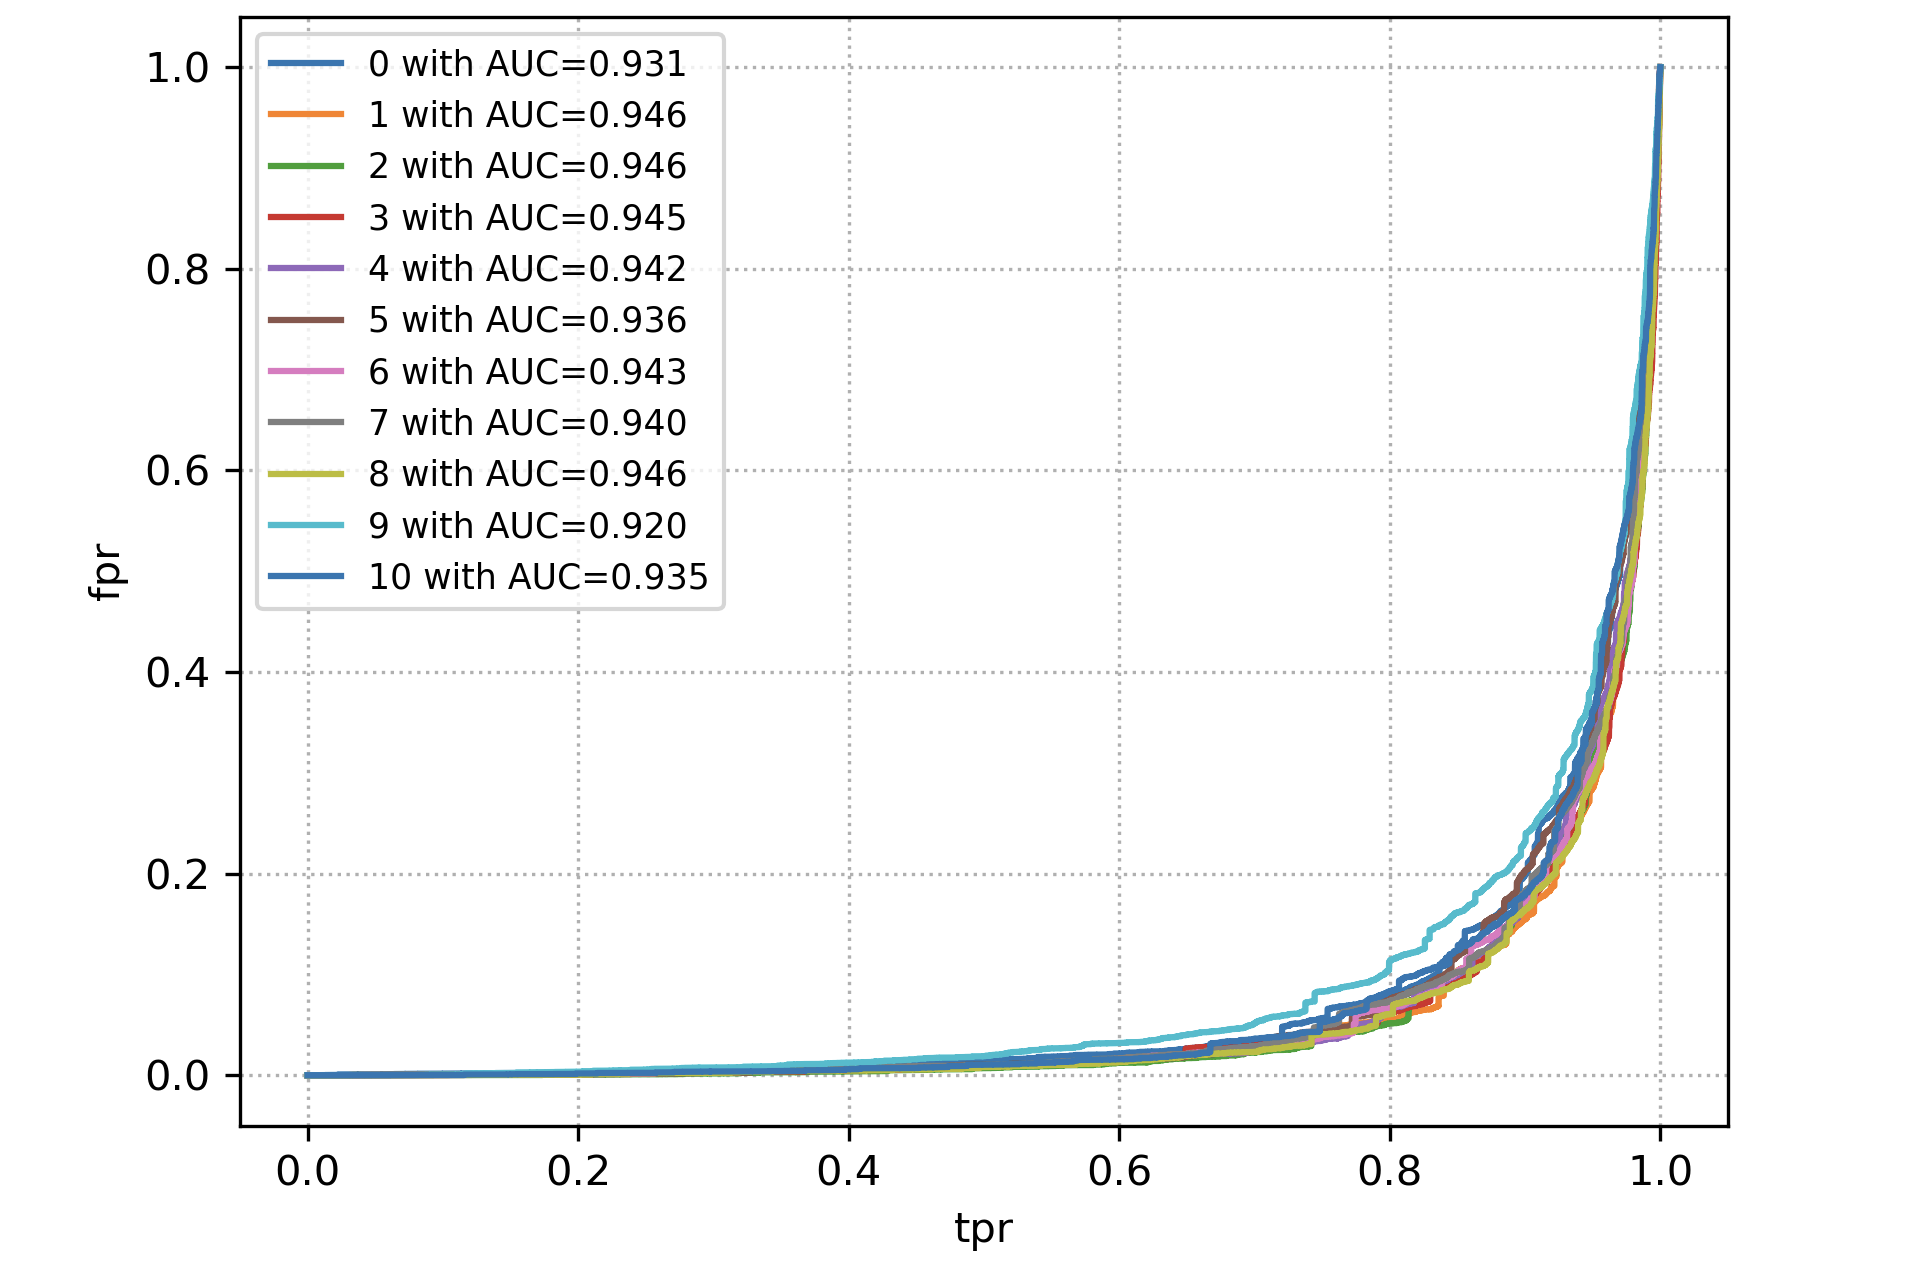
\includegraphics[width=1.1\linewidth]{Images/7.S_B/Variability/4b QCD prob diff and DNN.png}
  \caption{DNN and PD as global inputs}
  \label{fig: 4b QCD DNN PD}
\end{subfigure}
\caption{4b-QCD variability of the ROCs for the different inputs presented in Table \ref{table: S/B trainings}}
\label{fig: 4b QCD v ariability}
\end{figure}

\begin{figure}[hbt]
\centering
\begin{subfigure}{.5\textwidth}
  \centering
  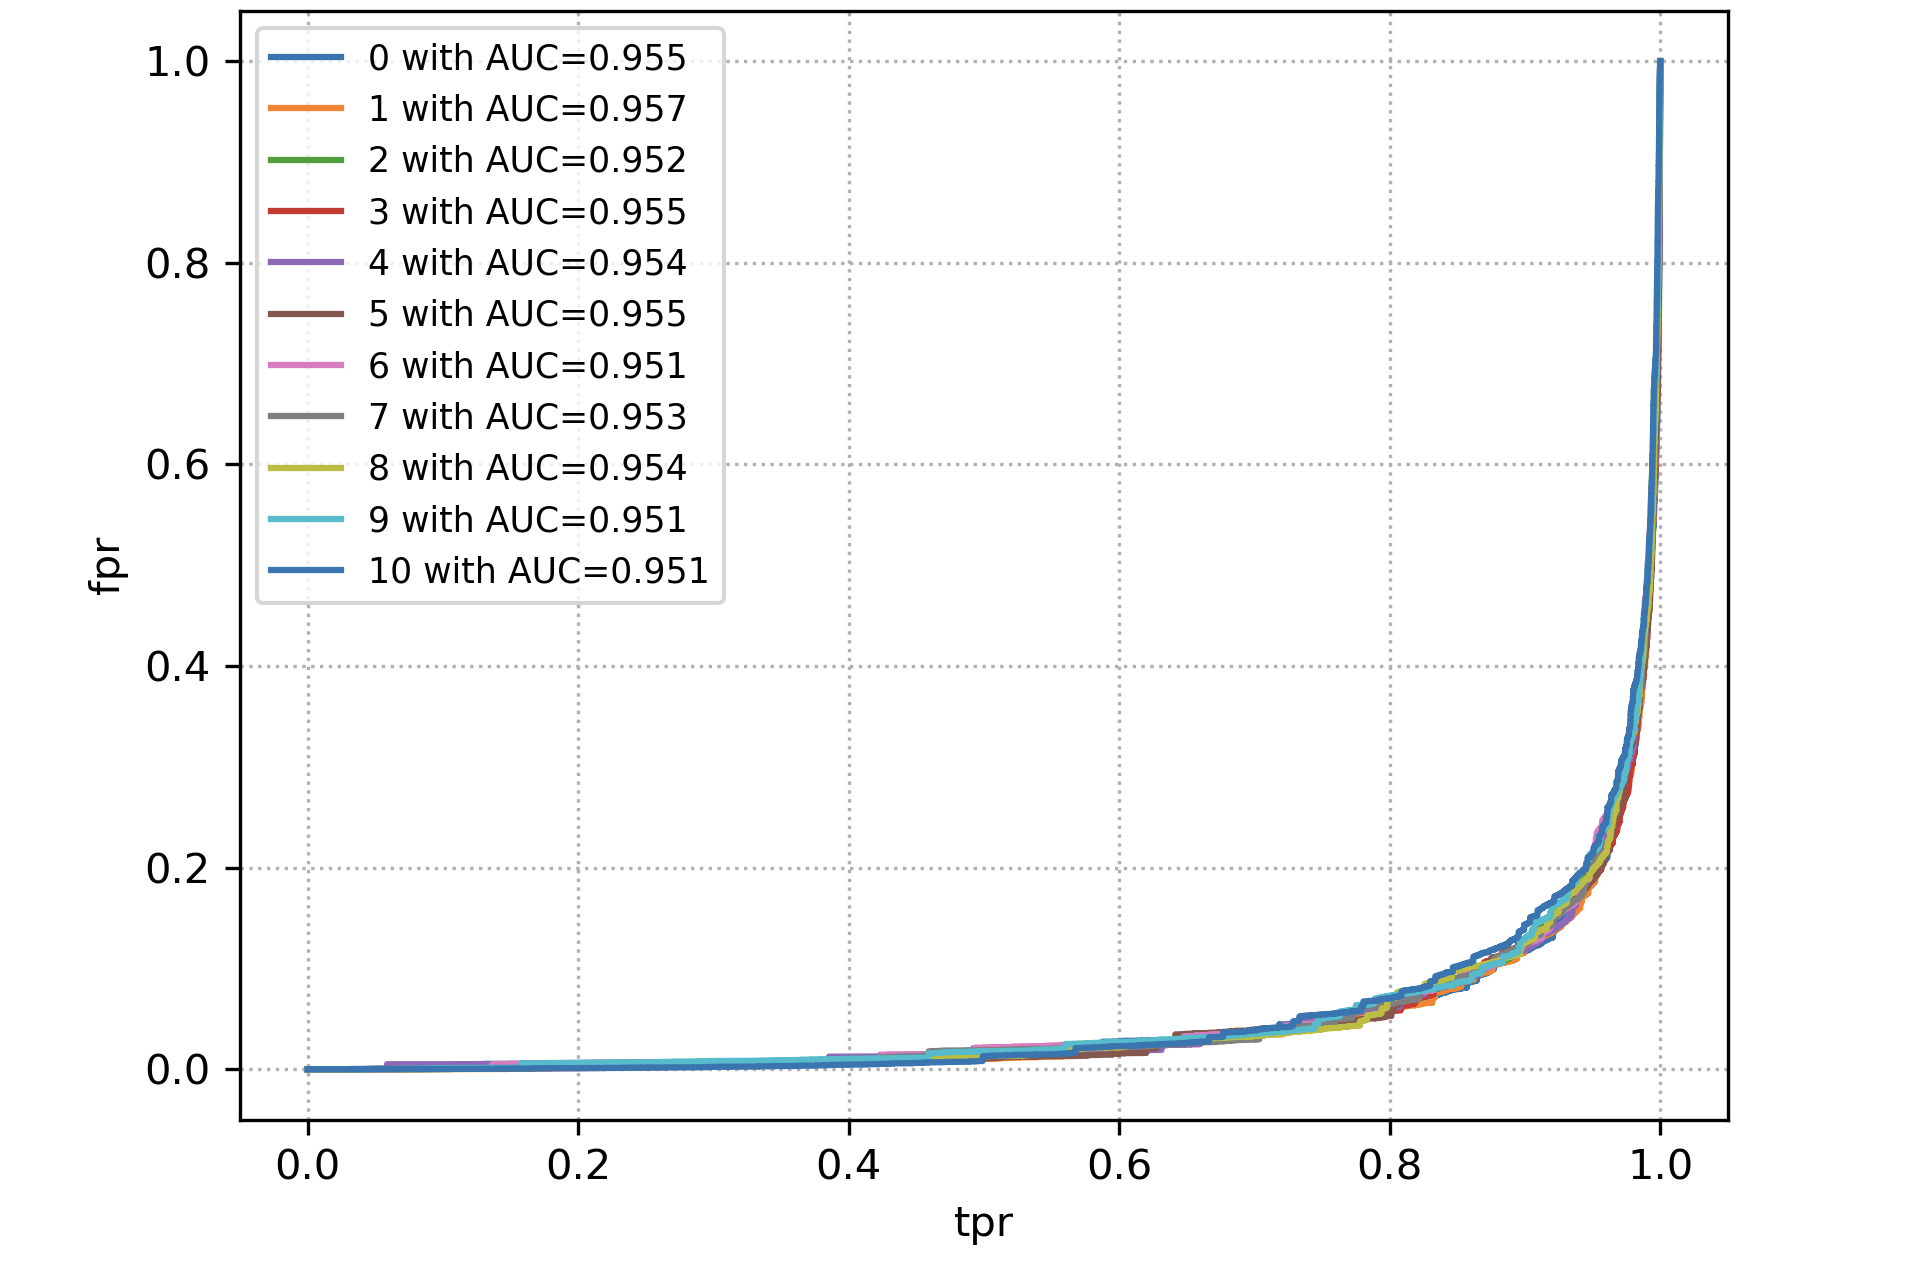
\includegraphics[width=1.1\linewidth]{Images/7.S_B/Variability/2b QCD DNN.png}
  \caption{DNN as global input}
  \label{fig: 2b QCD DNN}
\end{subfigure}%
\begin{subfigure}{.5\textwidth}
  \centering
  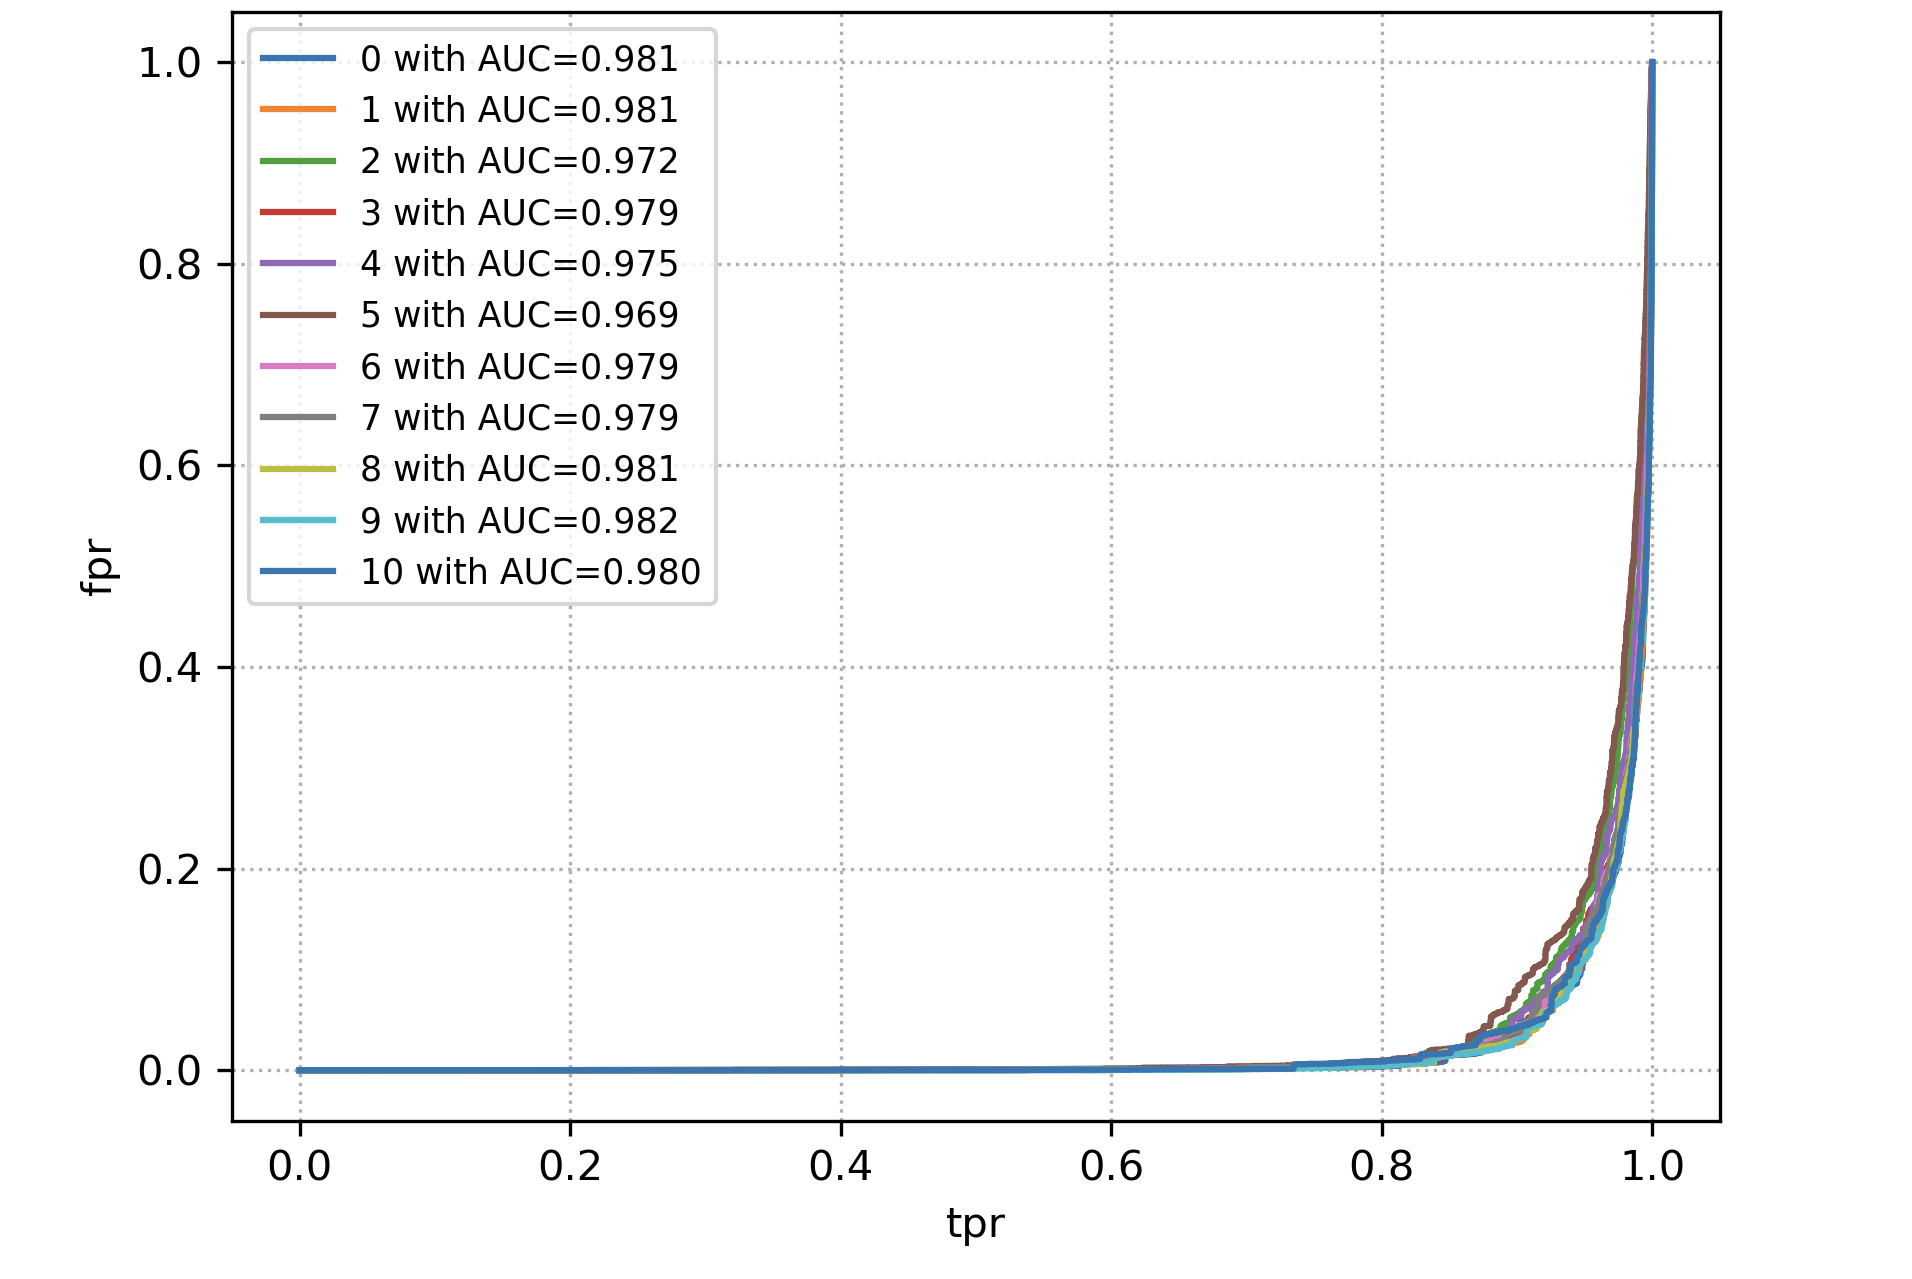
\includegraphics[width=1.1\linewidth]{Images/7.S_B/Variability/2b QCD DNN and prob diff.png}
  \caption{DNN and PD as global inputs}
  \label{fig: 2b QCD DNN PD}
\end{subfigure}
\caption{2b-QCD variability of the ROCs for the different inputs presented in Table \ref{table: S/B trainings}}
\label{fig: 2b QCD v ariability}
\end{figure}

\begin{figure}[hbt]
\centering
\begin{subfigure}{.5\textwidth}
  \centering
  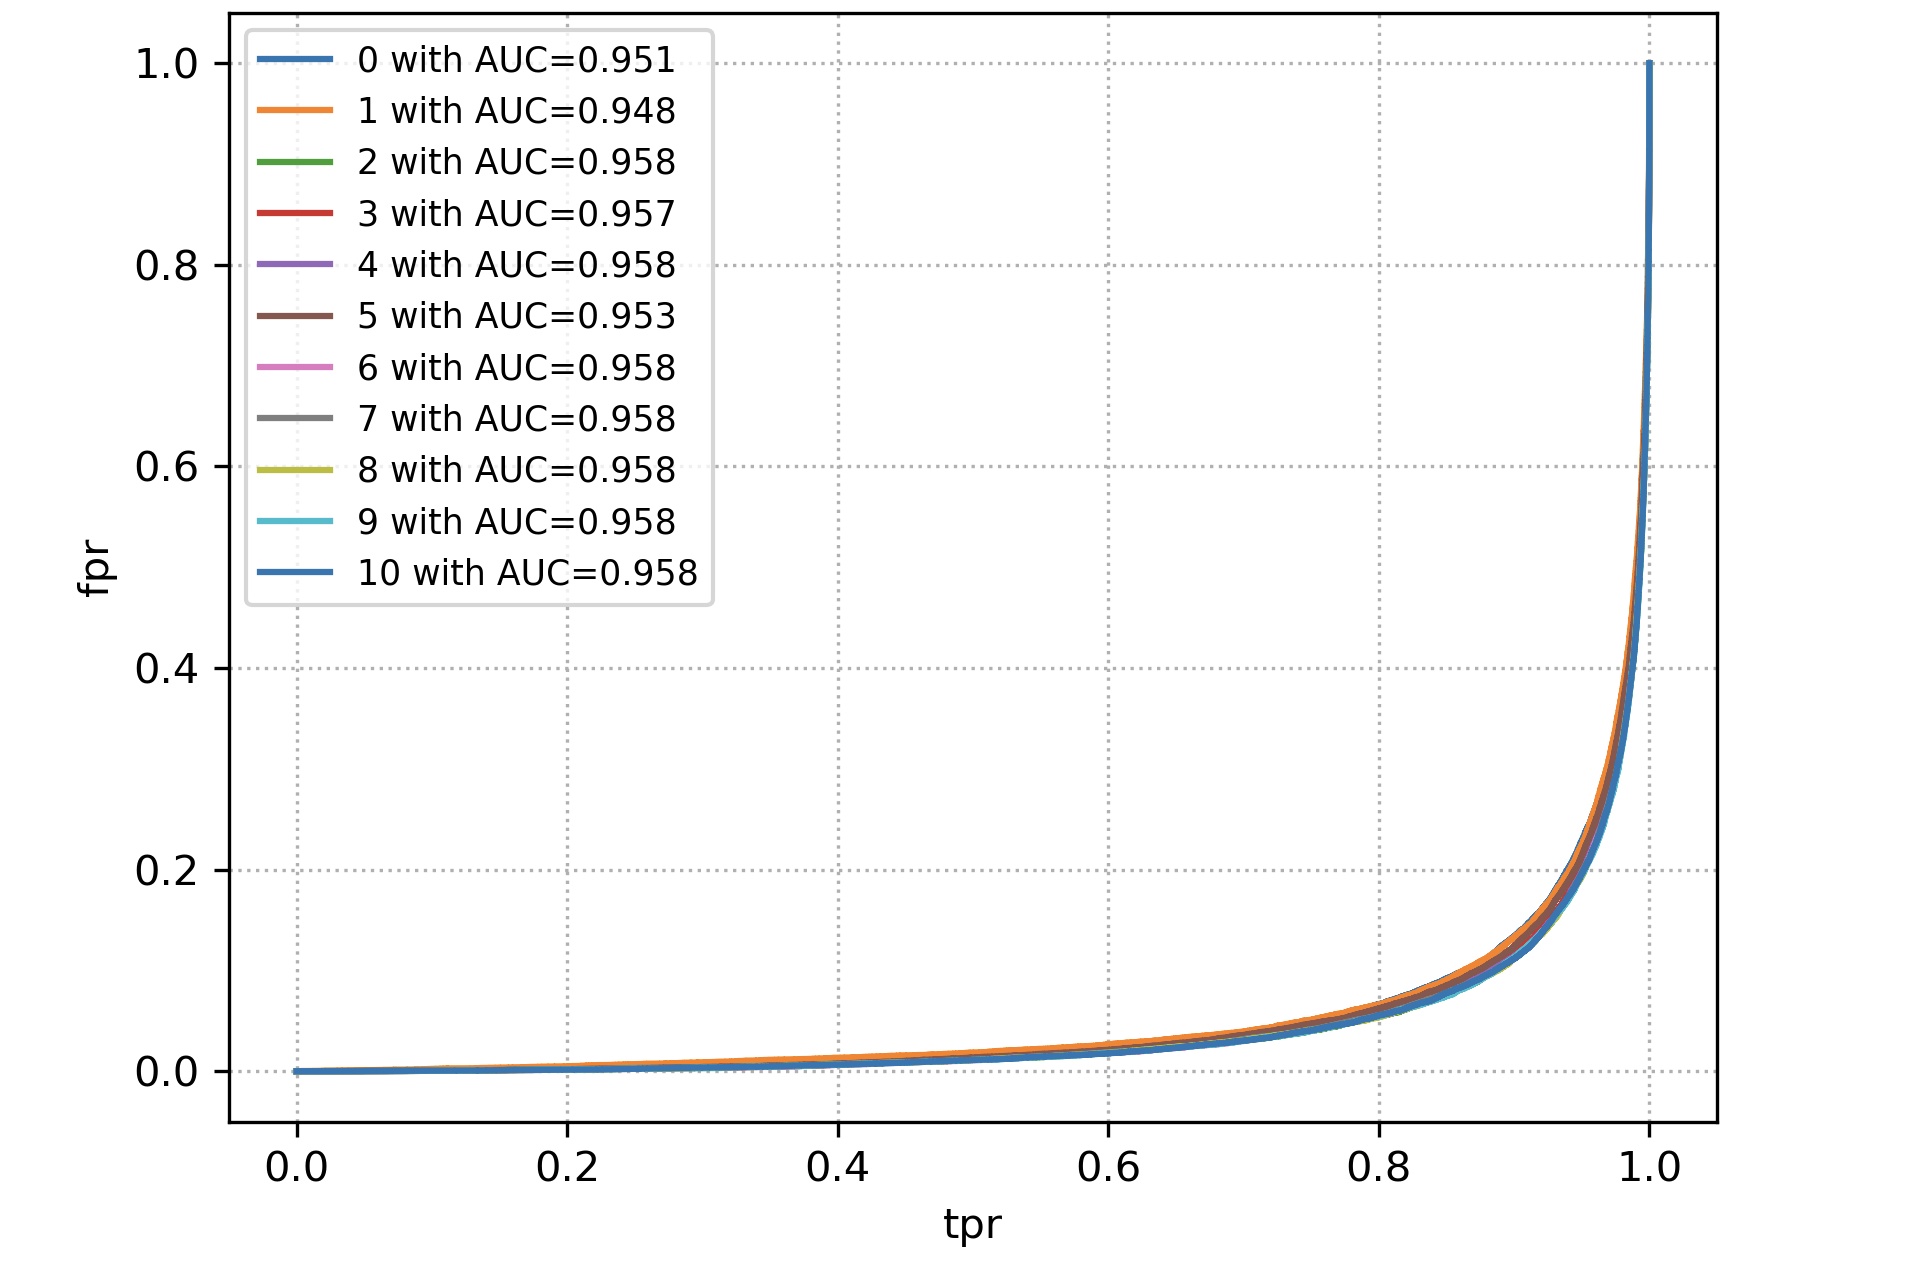
\includegraphics[width=1.1\linewidth]{Images/7.S_B/Variability/2b data DNN.png}
  \caption{DNN as global input}
  \label{fig: 2b data DNN}
\end{subfigure}%
\begin{subfigure}{.5\textwidth}
  \centering
  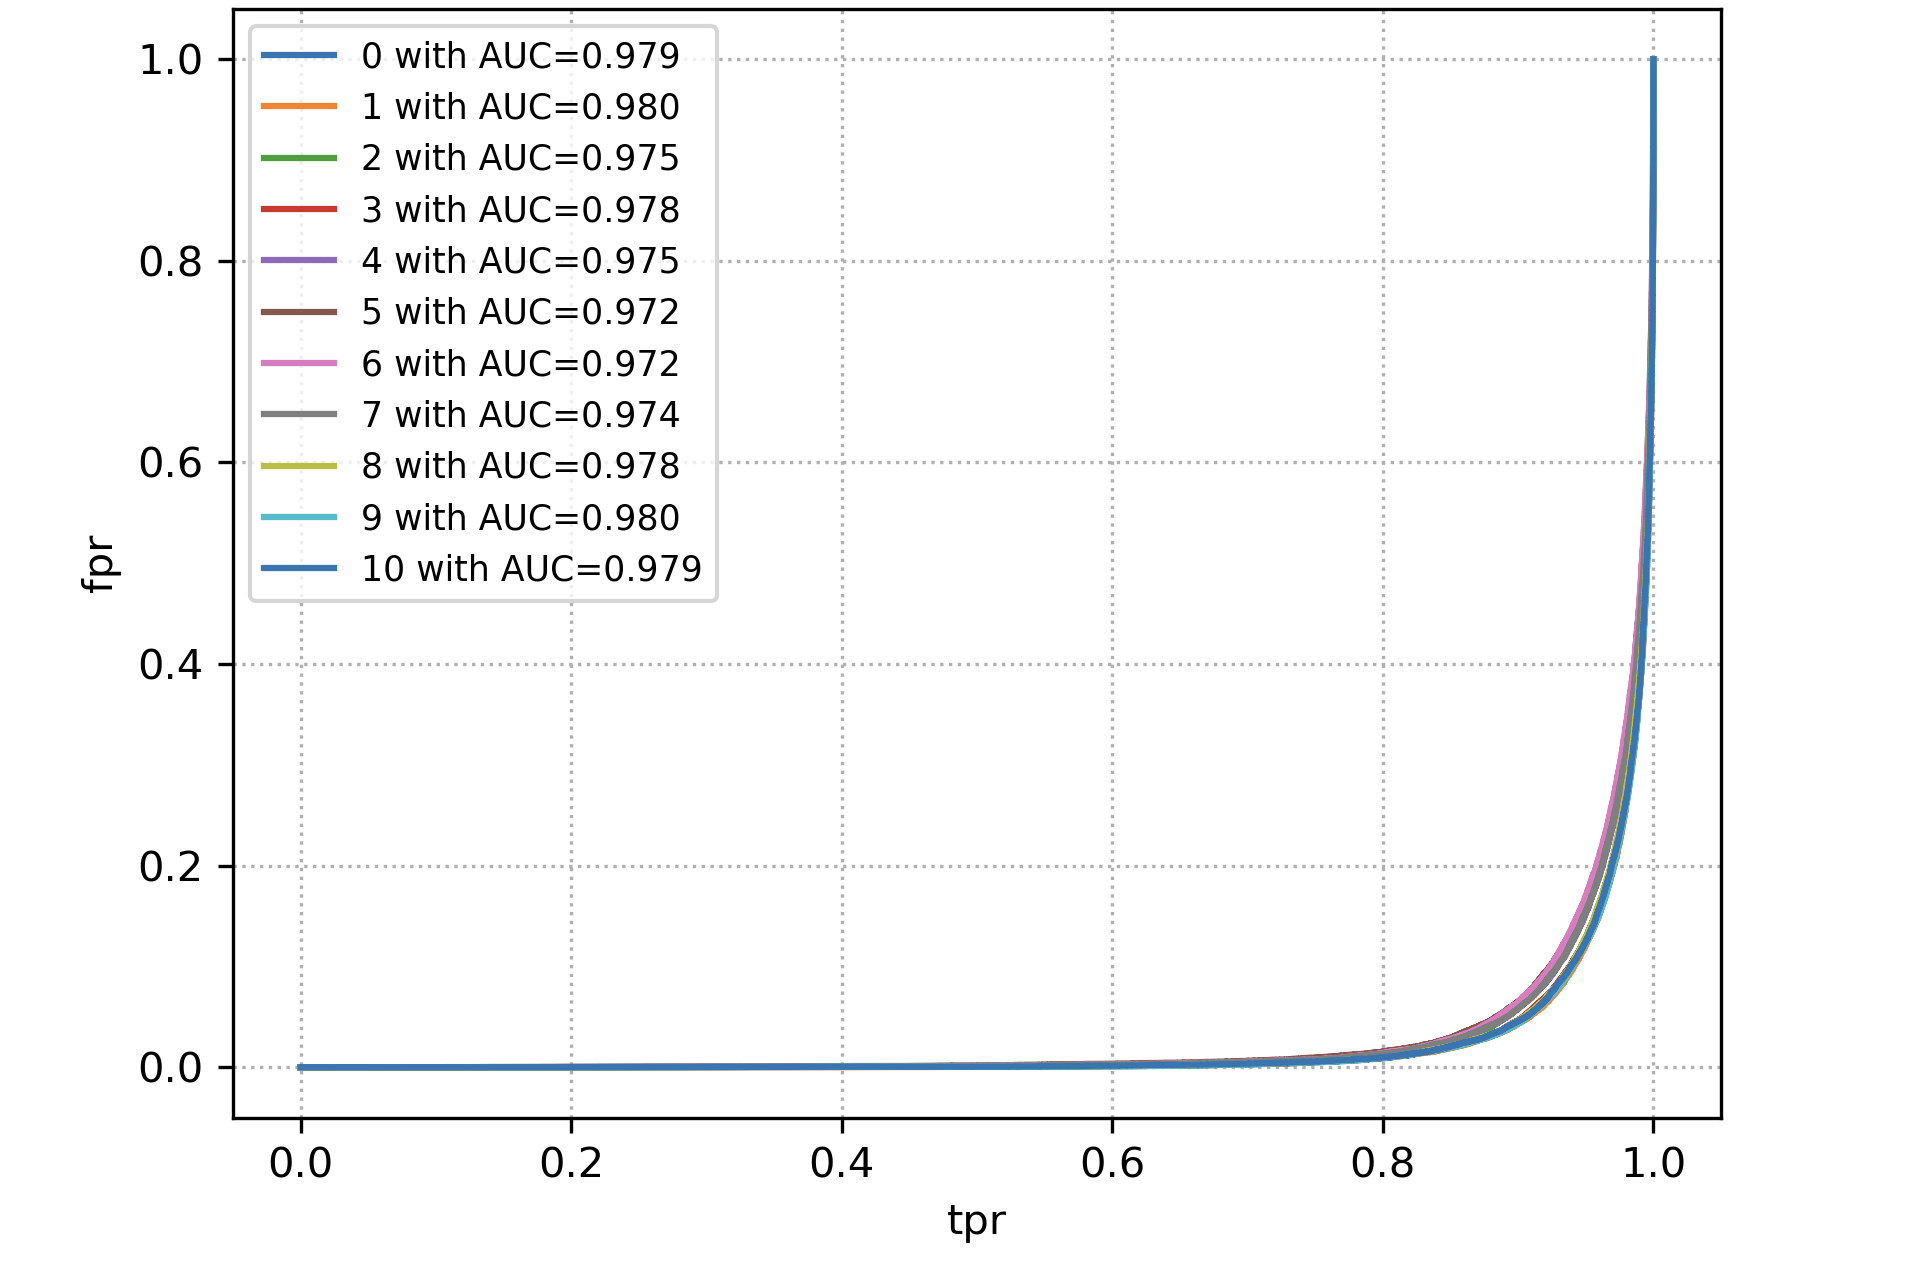
\includegraphics[width=1.1\linewidth]{Images/7.S_B/Variability/2b data DNN and prob diff.png}
  \caption{DNN and PD as global inputs}
  \label{fig: 2b data DNN PD}
\end{subfigure}
\caption{2b-data variability of the ROCs for the different inputs presented in Table \ref{table: S/B trainings}}
\label{fig: 2b data v ariability}
\end{figure}

\begin{table}[hbt]
\centering
\begin{tabular}{|M{5cm}||M{2.5cm}|M{2.5cm}|M{2.5cm}|}
 \hline
 Configuration  & Maximum value of the AUC & Minimum value of the AUC & Variability \\
 \hline
 \hline
 4b-QCD (DNN) & 0.949 & 0.932 & $\sim$0.017 \\
 \hline
 4b-QCD (DNN and PD) & 0.946 & 0.920 & $\sim$0.026 \\
 \hline
 \hline
 2b-QCD (DNN) & 0.957 & 0.951 & $\sim$0.008\\
 \hline
 2b-QCD (DNN and PD) & 0.982 & 0.969 & $\sim$0.013 \\
 \hline
 \hline
 2b-data (DNN) & 0.958 & 0.948 & $\sim$0.01 \\
 \hline
 2b-data (DNN and PD) & 0.980 & 0.972 & $\sim$0.008  \\
 \hline
\end{tabular}
\caption{Summary of the AUC values observed in Figures \ref{fig: 4b QCD v ariability}, \ref{fig: 2b QCD v ariability}, \ref{fig: 2b data v ariability} for the variability of the training presented in Table \ref{table: S/B trainings}}
\label{table: Spread of the trainings}
\end{table}


Due to some limitations in our available resources, we could not compute the variability for 2b data full statistics, nevertheless, we observed that the value of the AUC was not affected (within the variability of the training) by the difference in statistics, as is shown in Table \ref{table: 2b-data AUC r vs f}.


\begin{table}[hbt]
\centering
\begin{tabular}{|M{7cm}|M{4cm}|}
 \hline
 Configuration  & Value of the AUC \\
 \hline
 \hline
 2b-data reduced statistics (DNN) & 0.951  \\
 \hline
 2b-data full statistics (DNN) & 0.958 \\
\hline
 \hline
 2b-data reduced statistics (DNN and PD) & 0.979 \\
 \hline
 2b-data full statistics (DNN and PD) & 0.977  \\
\hline
\end{tabular}
\caption{Results of the AUC obtained after training SPANet on 2b-data full and reduced statistics}
\label{table: 2b-data AUC r vs f}
\end{table}


\subsection{4b data extrapolation} \label{subsection:4b data extrapolation inclusivce}

In the previous sections we presented the necessary results to compute the 4b data extrapolation as was explained in section \ref{subsection: sample dep}. Since we don't have an immediate solution to reduce the variability on the 4b-QCD trainings, as a first approximation for the extrapolation we will compute the b-tag ratio in Eq.(\ref{eq: extrapolation}) (\textcolor{BlueGreen}{blue}) for the 11 seeds and see where the value from the AN stands within this variability.

In Figures \ref{fig: 4b data extrapolation DNN} and \ref{fig: 4b data extrapolation DNN PD} we present the results of the extrapolation and the comparison to the ROC in the AN. The values of the AUC reported in these plots are the extrapolated values computed using Eq.(\ref{eq: extrapolation}). We only show in these plots the best and the worst performing ROCs of our training to see with more clarity where the AN ROC stands within the variability of our training. By looking at these figures we can conclude that using the PD variable does not improve our performance. For both cases, the results from the AN are within the variability of our trainings. 

\begin{figure}[hbt]
    \centering
    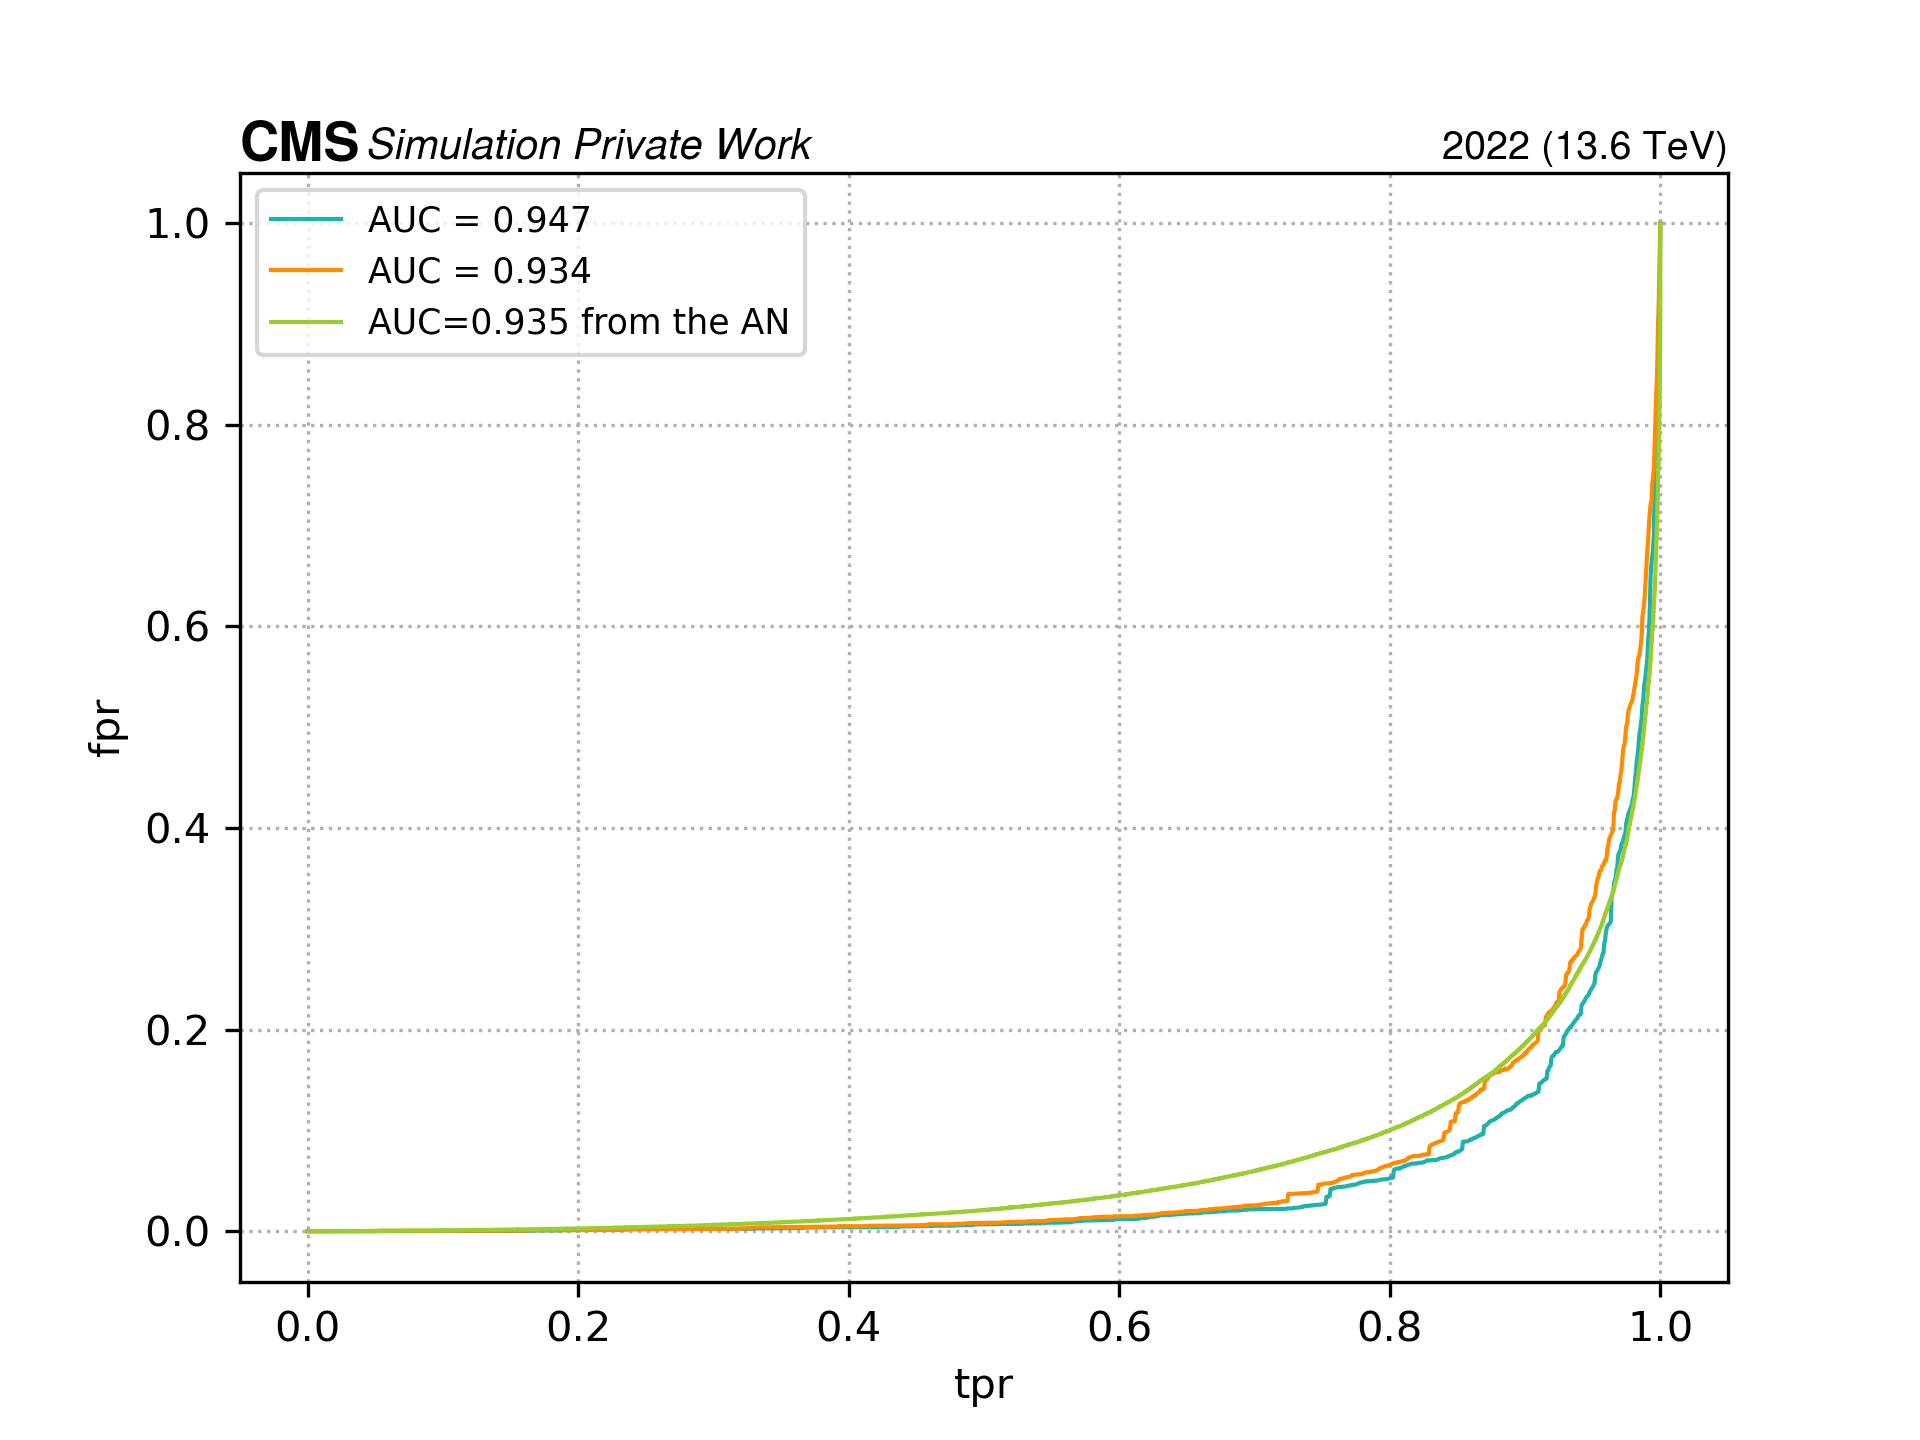
\includegraphics[width=0.7\linewidth]{Images/7.S:B/Extrapolation/4b data dnn.png}
    \caption{Extrapolation to 4b data using the training with 2b data full statics, 2b data reduced statistics, 2b QCD reduced statistics and 4b-QCD with DNN variables as inputs. The FPR is computed using Eq.(\ref{eq: extrapolation}) and TPR is the one from 2b data full statistics. The AUCs showed in this figure are the extrapolated using Eq.(\ref{eq: extrapolation})}
    \label{fig: 4b data extrapolation DNN}
\end{figure}

\begin{figure}[hbt]
    \centering
    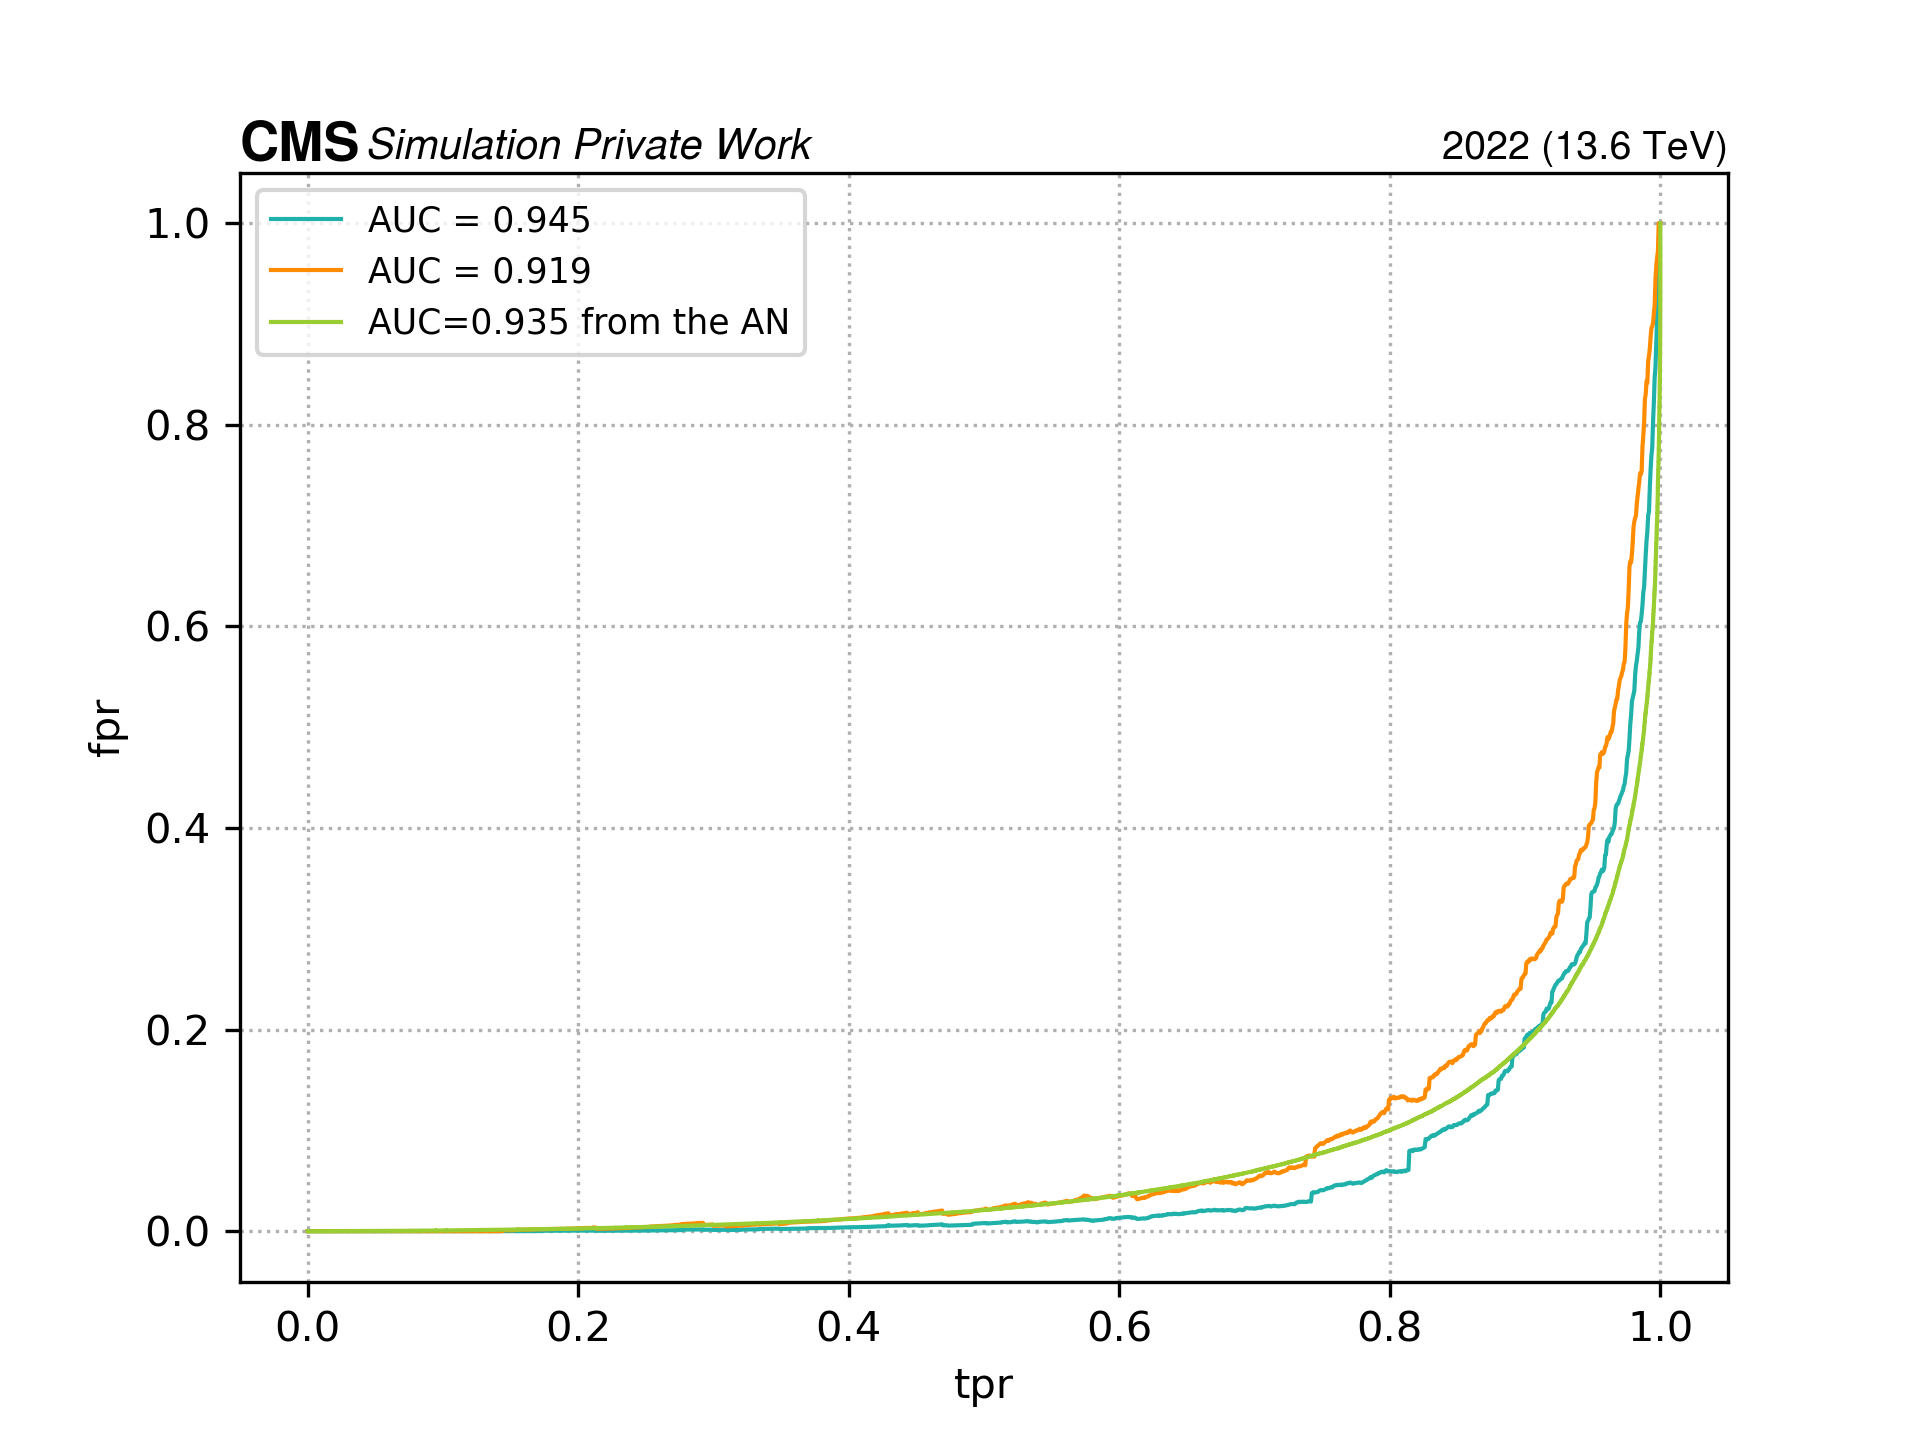
\includegraphics[width=0.7\linewidth]{Images/7.S:B/Extrapolation/4b data dnn proba.png}
    \caption{Extrapolation to 4b data using the training with 2b data full statics, 2b data reduced statistics, 2b QCD reduced statistics and 4b-QCD with DNN and PD variables as inputs. The FPR is computed using Eq.(\ref{eq: extrapolation}) and TPR is the one from 2b data full statistics. The AUCs showed in this figure are the extrapolated using Eq.(\ref{eq: extrapolation}}
    \label{fig: 4b data extrapolation DNN PD}
\end{figure}

(Do I also compare here best vs best and worse vs worse? As done in the last section for the SR)

\clearpage

\subsection{Signal region}

So far we have trained our models inclusively and we have been comparing them to the results in the AN. Nevertheless, the results in the AN have been obtained by training the DNN with samples considering only events in the SR (defined in section \ref{section: HH4b}). We will start by evaluating our current inclusive models presented in the previous section in samples with events in the SR and then trained and evaluated in the SR samples.


\subsubsection{Evaluation on SR}

Before we could perform our trainings with a SR sample, we started by evaluating our inclusive trainings on SR test samples. We started by comparing the evaluation of our training in 2b-data full statistics inclusive or 2b-data full statistics in the SR. The results are shown in Figure \ref{fig: 2b data comparison ev on SR}. We can see from this figure that for the training using DNN and PD as global variables, the performance is the same on SR or inclusively (within the variability). Nevertheless, for 2b-data using only DNN as inputs we observe a significant loss in performance.

\begin{figure}[hbt]
    \centering
    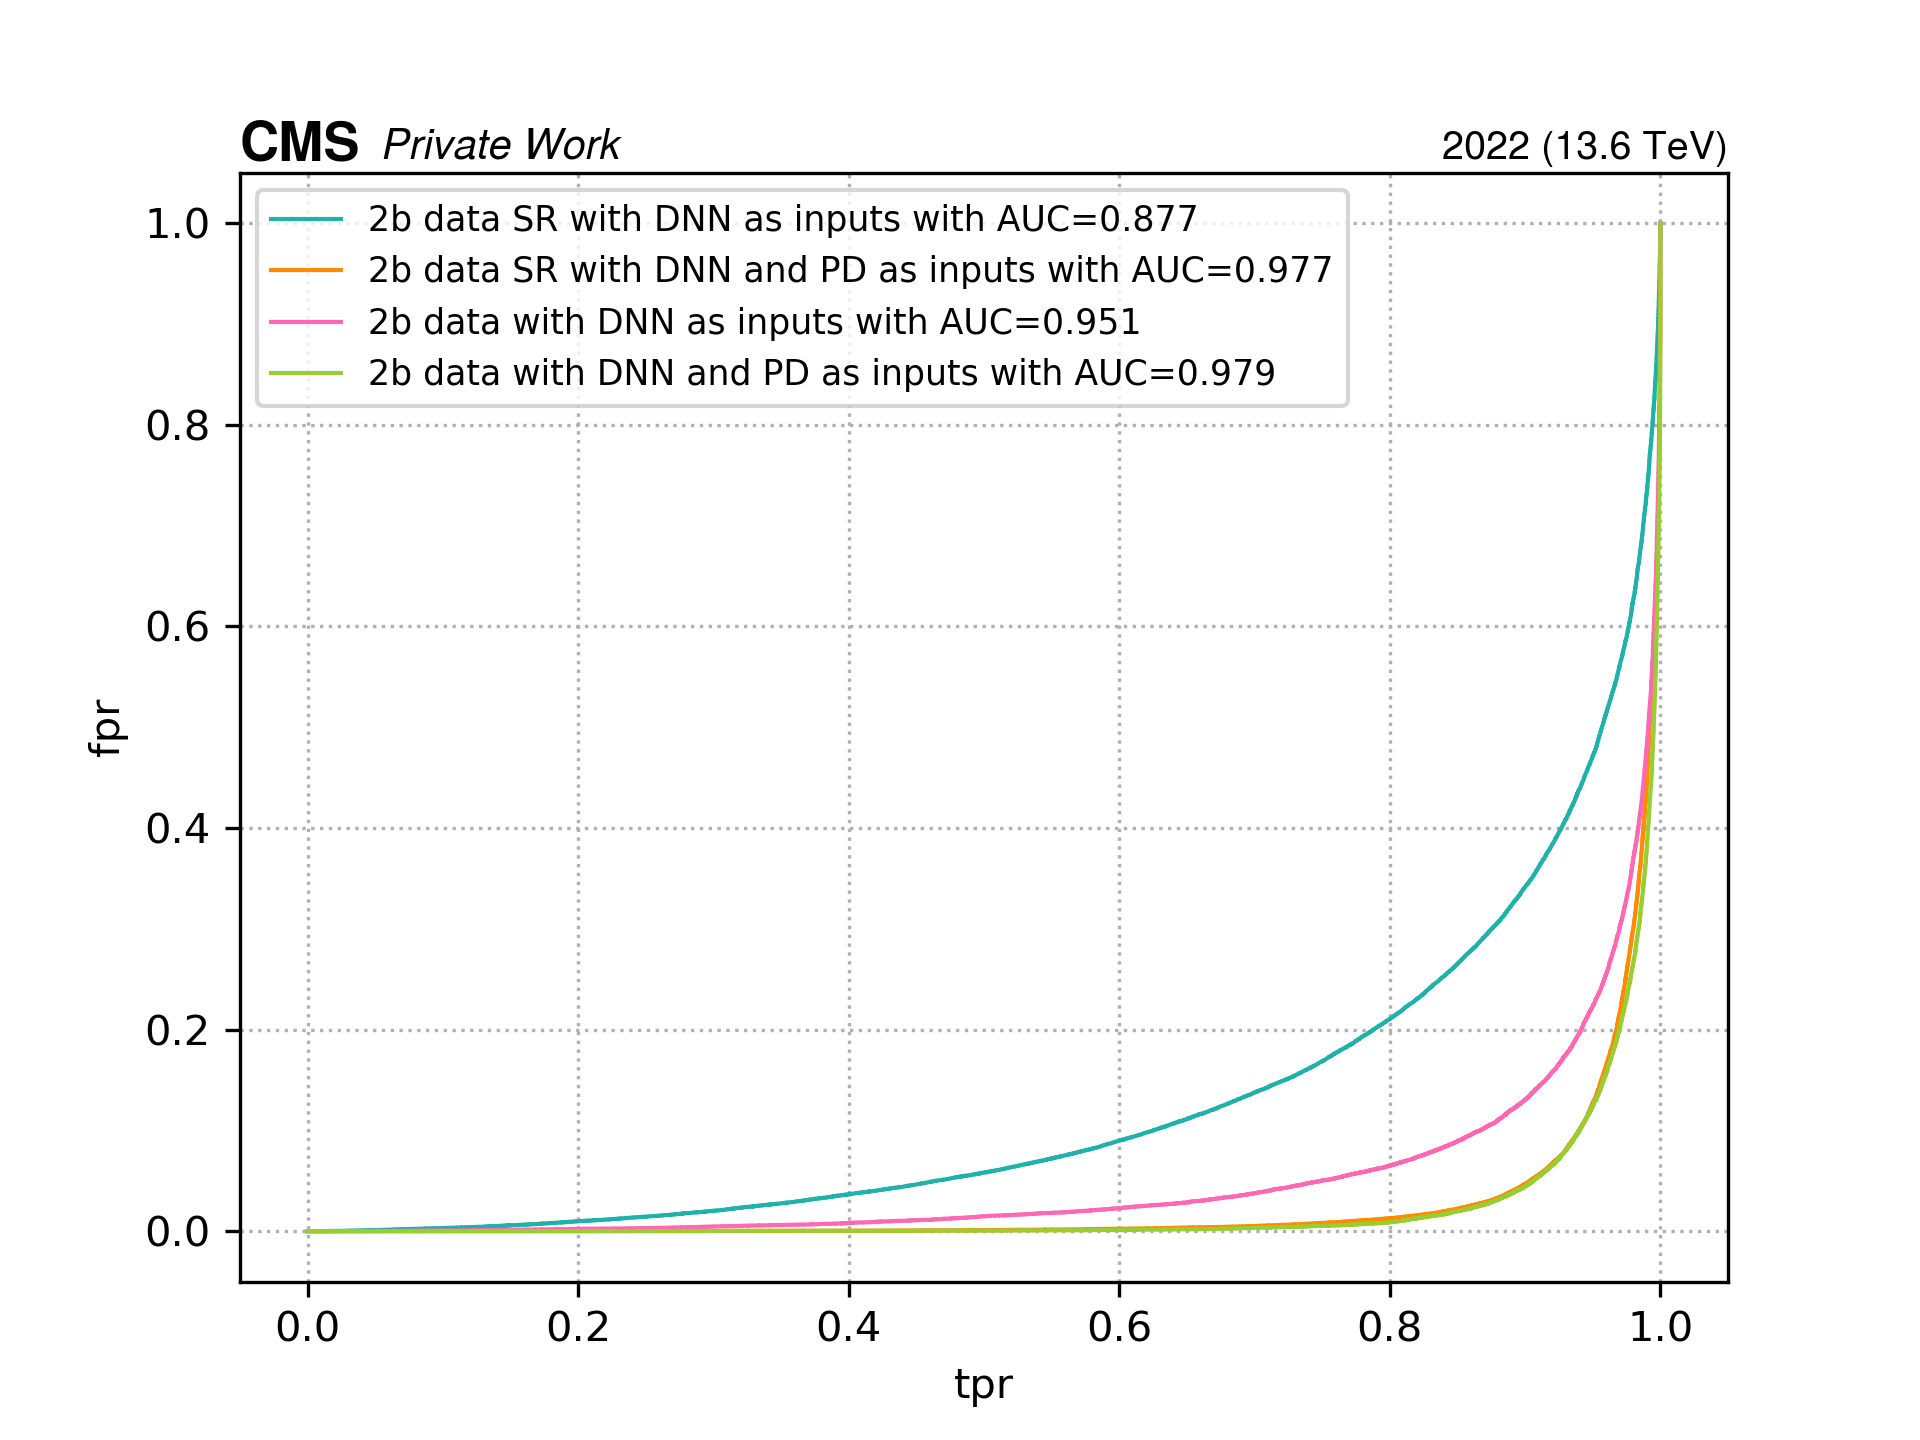
\includegraphics[width=0.7\linewidth]{Images/7.S:B/SR stats/2b-data comp.png}
    \caption{Comparison of the models trained inclusively with the 2b-data configuration evaluated inclusively and in the SR. The samples named 2b data SR are the ones containing only events in the SR}
    \label{fig: 2b data comparison ev on SR}
\end{figure}

Moreover in Figures \ref{fig: ev on SR dnn pd} and \ref{fig: ev on SR dnn pd}, we show the extrapolation to the 4b-data when evaluating on SR samples. Nevertheless, we can see that our performance worsens significantly, therefore we conclude that in order to have better performance we need to perform the trainings and evaluations on SR samples as will be shown in the next section.

\begin{figure}[hbt]
    \centering
    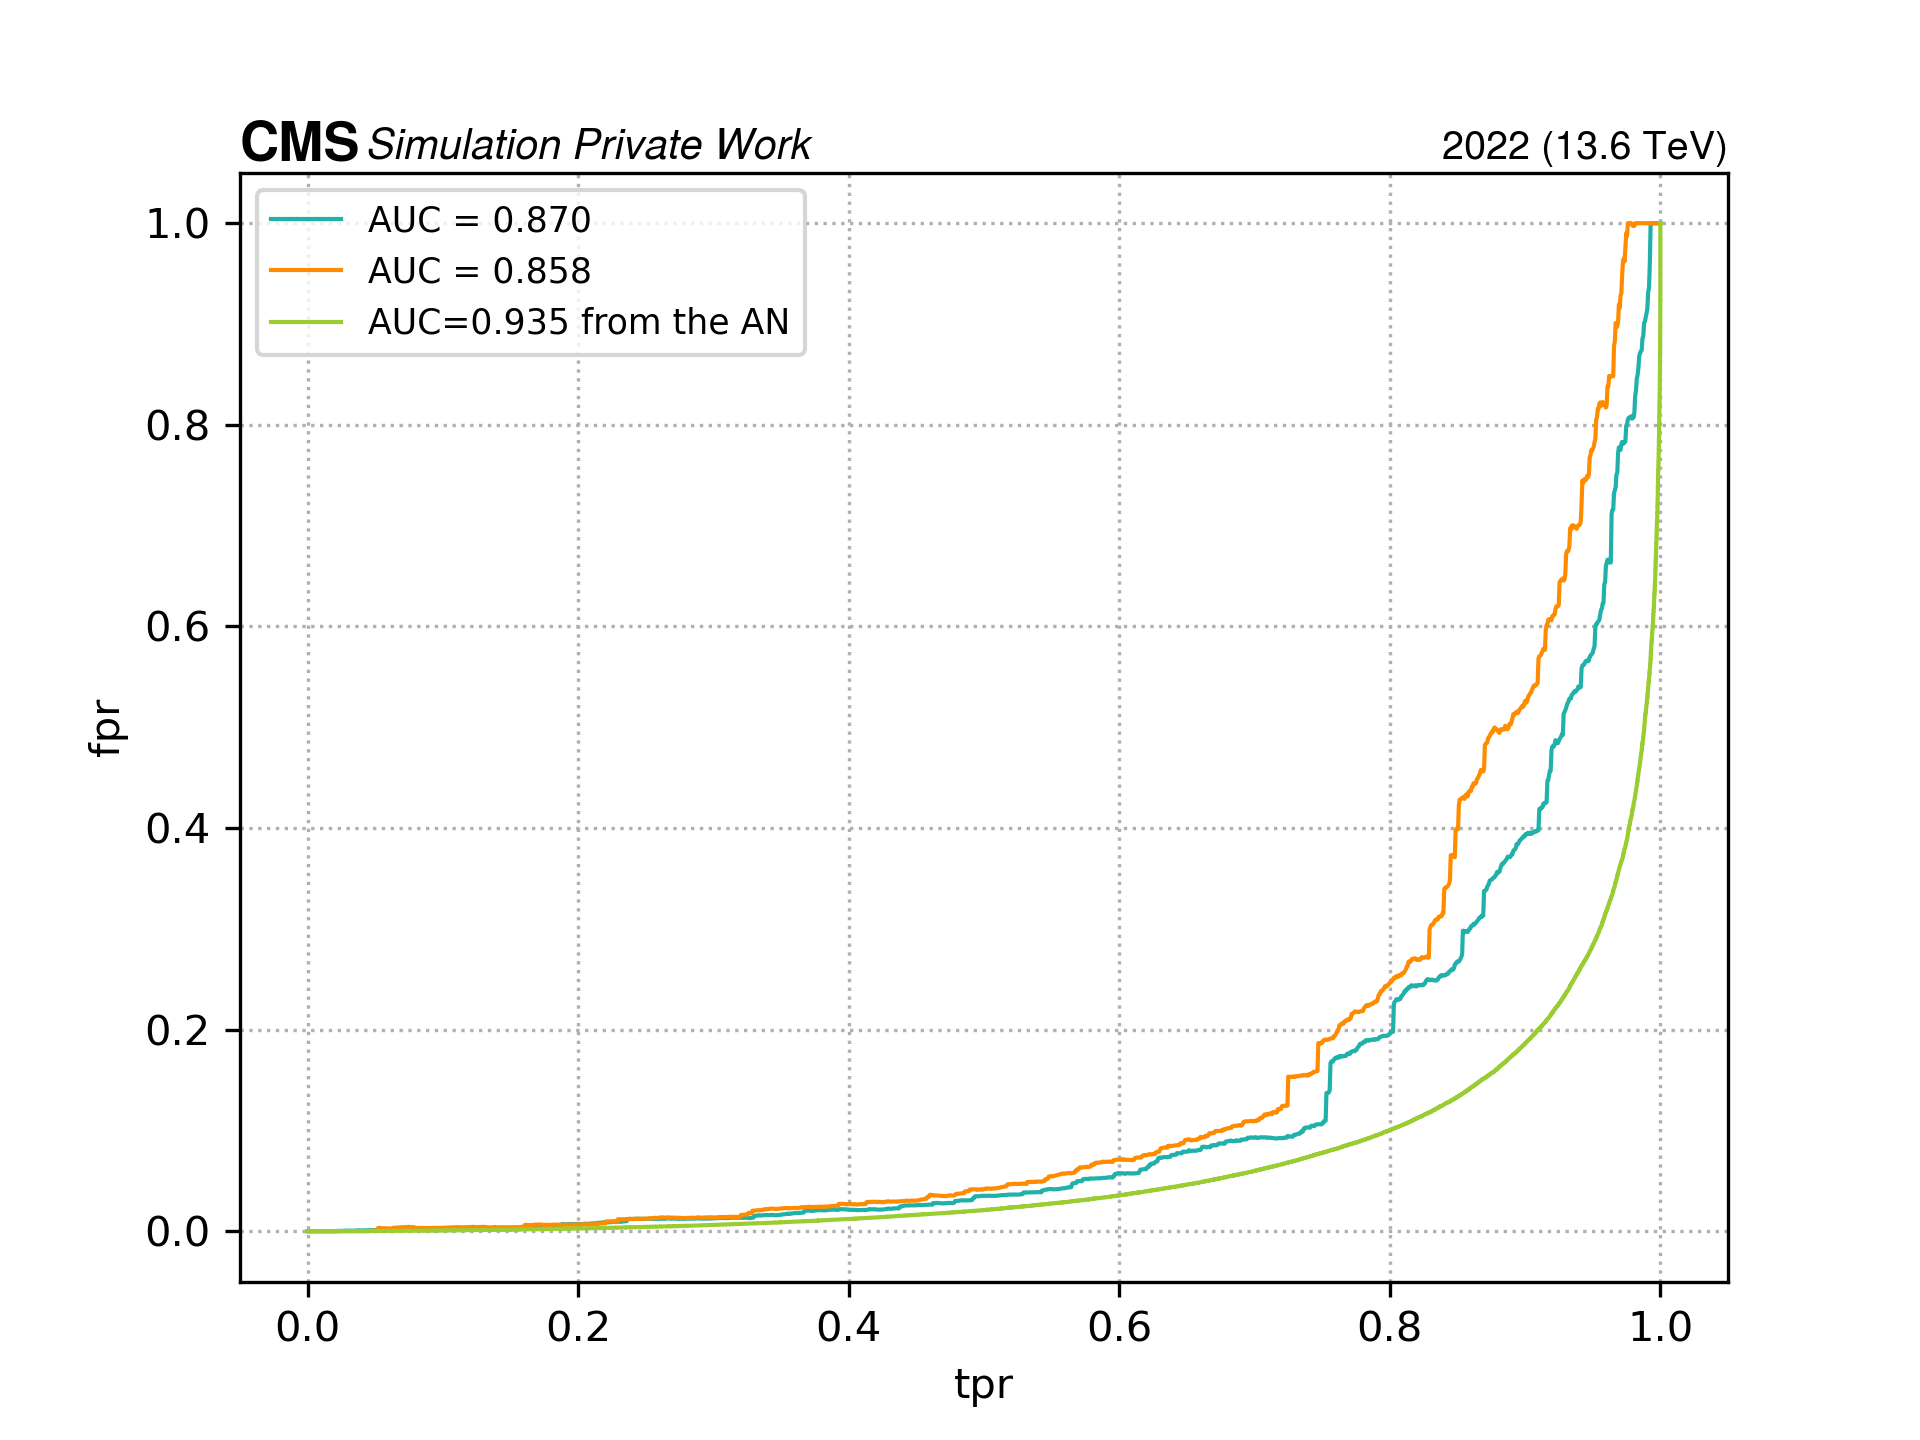
\includegraphics[width=0.7\linewidth]{Images/7.S:B/SR stats/4b data extrapol ev on SR dnn.png}
    \caption{Extrapolation to 4b data using the inclusive trainings with 2b data full statics, 2b data reduced statistics, 2b QCD reduced statistics and 4b-QCD with DNN variables as inputs but evaluated on SR. The FPR is computed using Eq.(\ref{eq: extrapolation}) and TPR is the one from 2b data full statistics. The AUCs showed in this figure are the extrapolated using Eq.(\ref{eq: extrapolation})}
    \label{fig: ev on SR dnn pd}
\end{figure}

\begin{figure}[hbt]
    \centering
    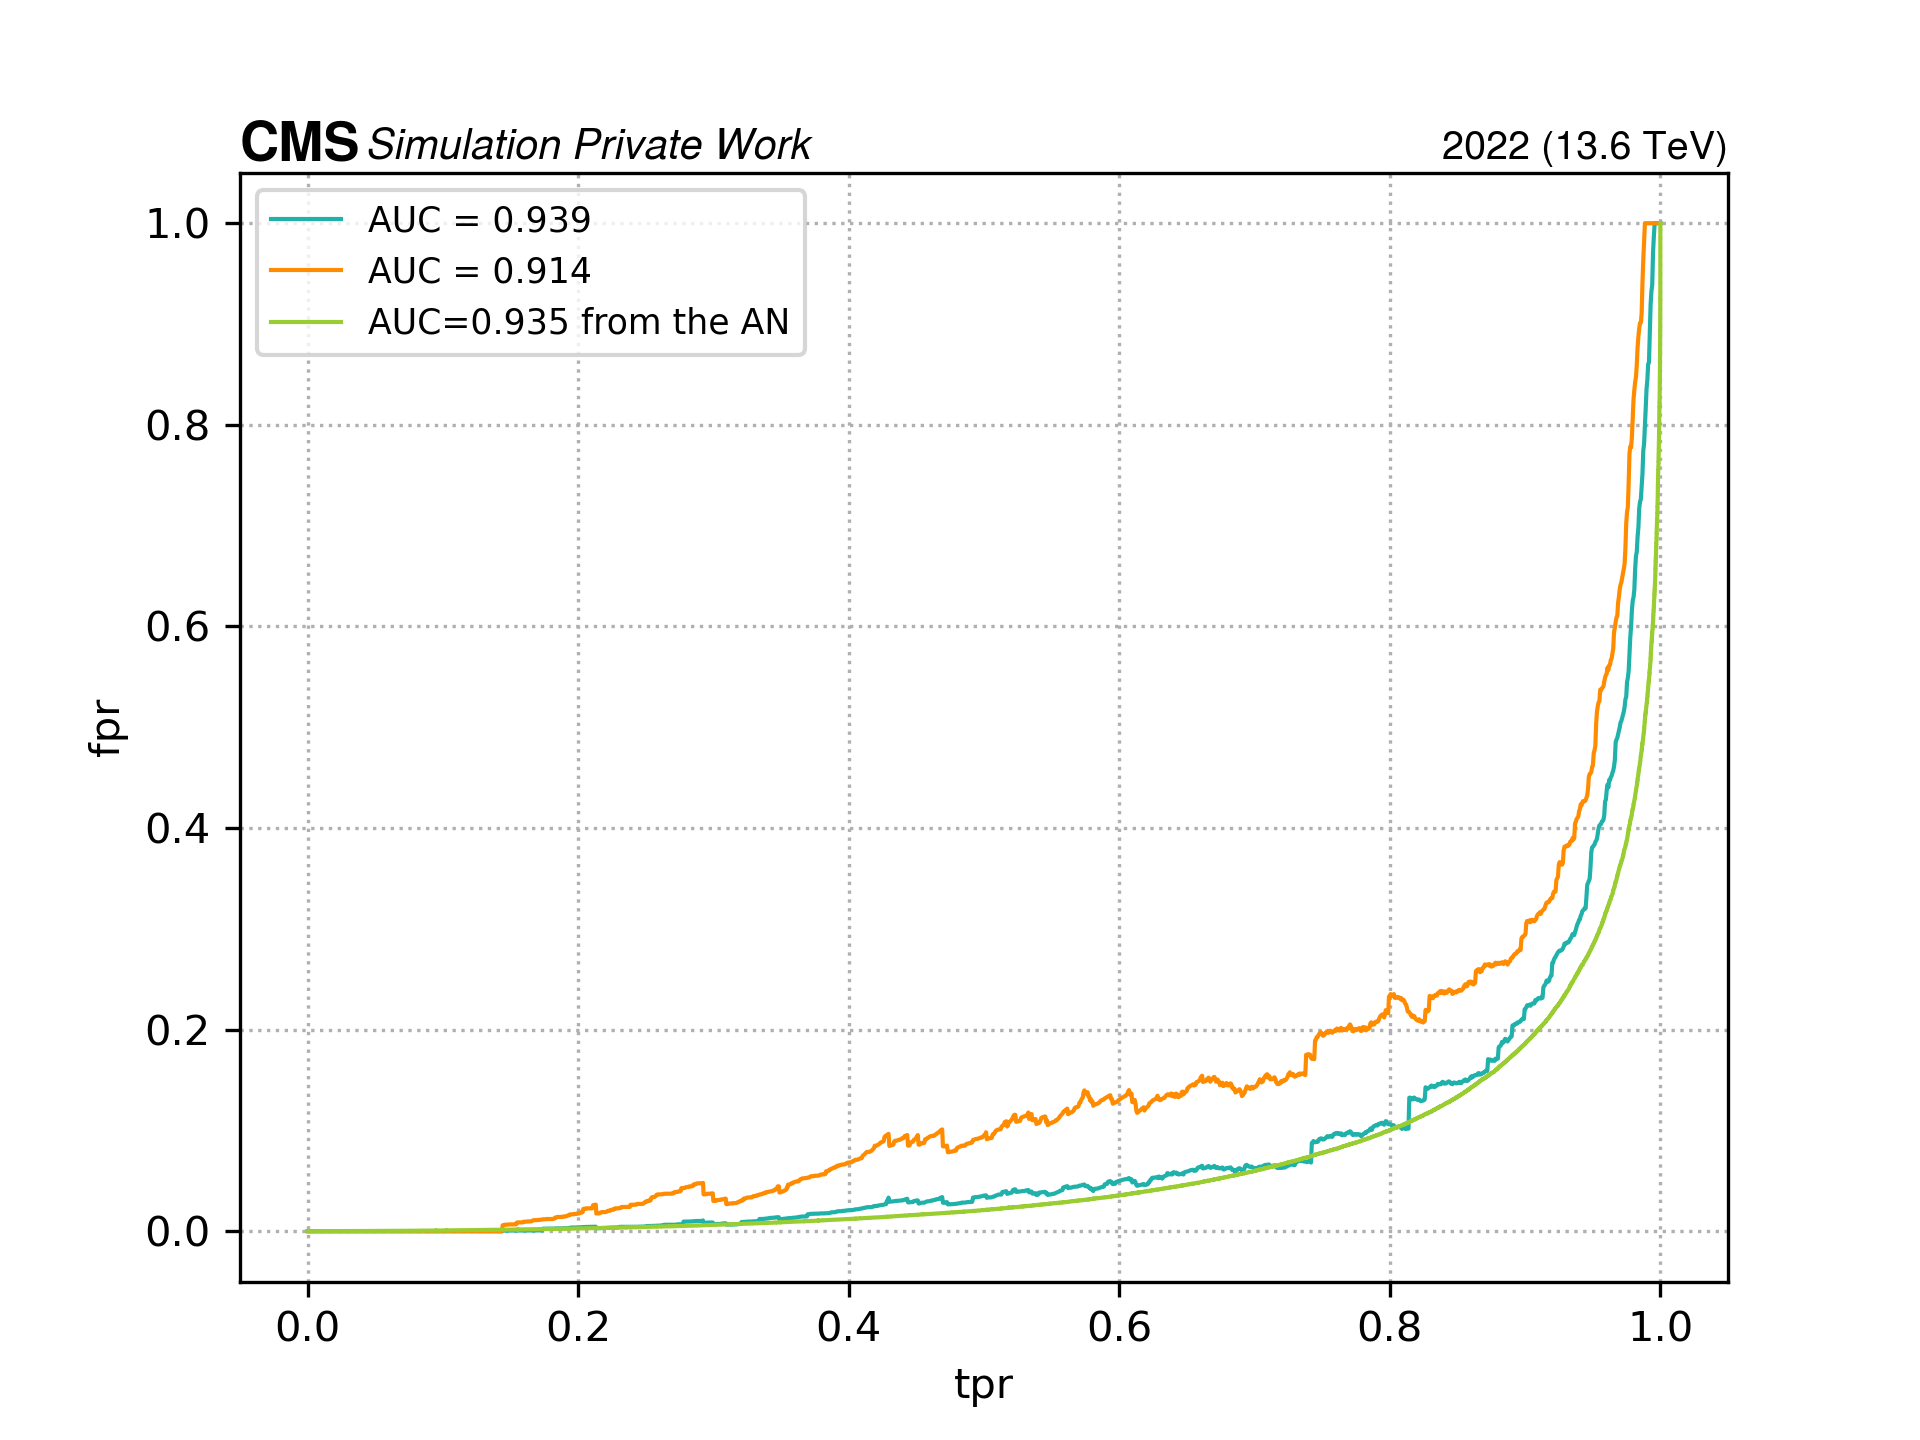
\includegraphics[width=0.7\linewidth]{Images/7.S:B/SR stats/4b data extrapolation dnn proba ev on sr.png}
    \caption{Extrapolation to 4b data using the inclusive trainings with 2b data full statics, 2b data reduced statistics, 2b QCD reduced statistics and 4b-QCD with DNN and PD variables as inputs but evaluated on SR. The FPR is computed using Eq.(\ref{eq: extrapolation}) and TPR is the one from 2b data full statistics. The AUCs showed in this figure are the extrapolated using Eq.(\ref{eq: extrapolation})}
    \label{fig: ev on SR dnn pd}
\end{figure}

\clearpage


\subsubsection{Training and evaluation on SR}

When performing the trainings in the SR it is important to point out that, as can be seen in Table \ref{table: SR efficiency}, the SR efficiency is very little for the background, hence, we are left with very little statistics.

\begin{table}[hbt]
\centering
\begin{tabular}{|M{3cm}||M{3.5cm}|M{3.5cm}|M{3.5cm}|}
 \hline
 Sample  & Number of events after preselections & Number of events in the SR & SR efficiency\\
 \hline
 \hline
 4b-Signal & 800k & 540k & 67\%\\
 \hline
 4b-QCD & 120k & 10k & 8\% \\
 \hline
 4b-data & 130k &  &  \\
 \hline
 \hline
 2b-Signal & 420k & & \\
 \hline
 2b-QCD & 4.4M & 220k & 5\% \\
 \hline
 2b-data & 5.9M & 470k & 8\% \\
 \hline
\end{tabular}
\caption{Signal region efficiency for the different configurations used for the SPANet trainings}
\label{table: SR efficiency}
\end{table}

We show in Figure \ref{fig: Assigned prob 4b QCD SR} the probability assigned by SPANet after performing a training with the 4b-QCD configuration using only events in the signal region, that we will refer to as the 4b-QCD-SR configuration. In this case we used the DNN and PD variables as inputs. As we can observe in this figure, when considering the weighted events, we have very significant fluctuations of the background due to the lack of statistics. This is then reflected on the ROC of this distribution as can be seen in Figure \ref{fig: ROC of the assignment proba SR}.  The same feature is observed when using only DNN as input variables.

\begin{figure}[hbt]
    \centering
    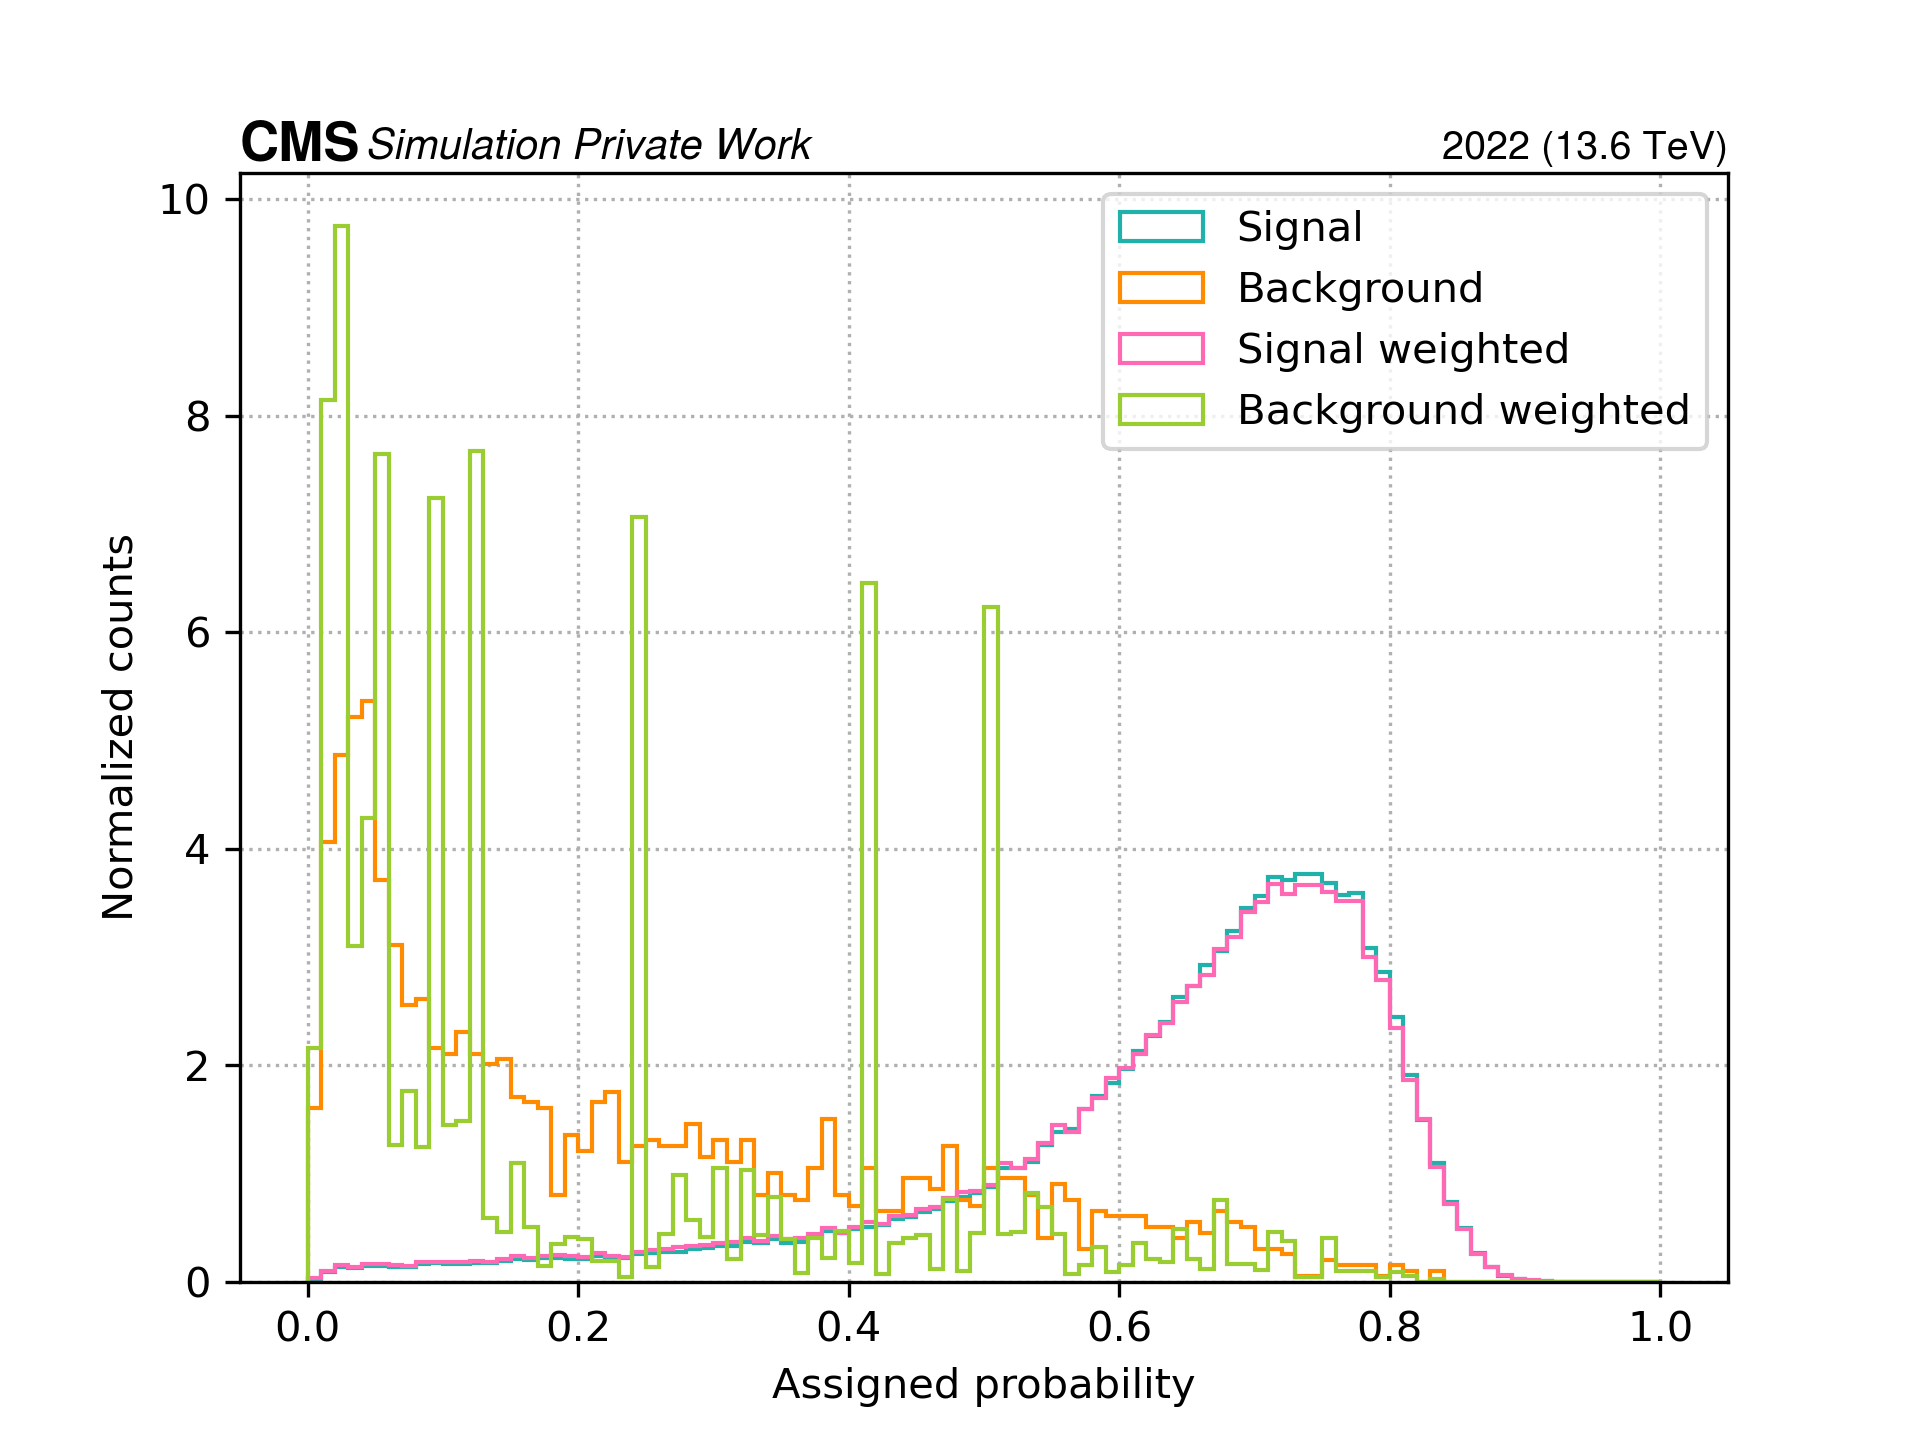
\includegraphics[width=0.7\linewidth]{Images/7.S:B/SR stats/4b stats SR class output.png}
    \caption{Probability assigned by SPANet as classifier of the signal events in the SR as well as the 4b QCD background events in the signal region. For this training we used DNN and PD variables as global inputs. Due to the lack of statistics in the background, we observe big fluctuations in the weighted distribution}
    \label{fig: Assigned prob 4b QCD SR}
\end{figure}

\begin{figure}[hbt]
    \centering
    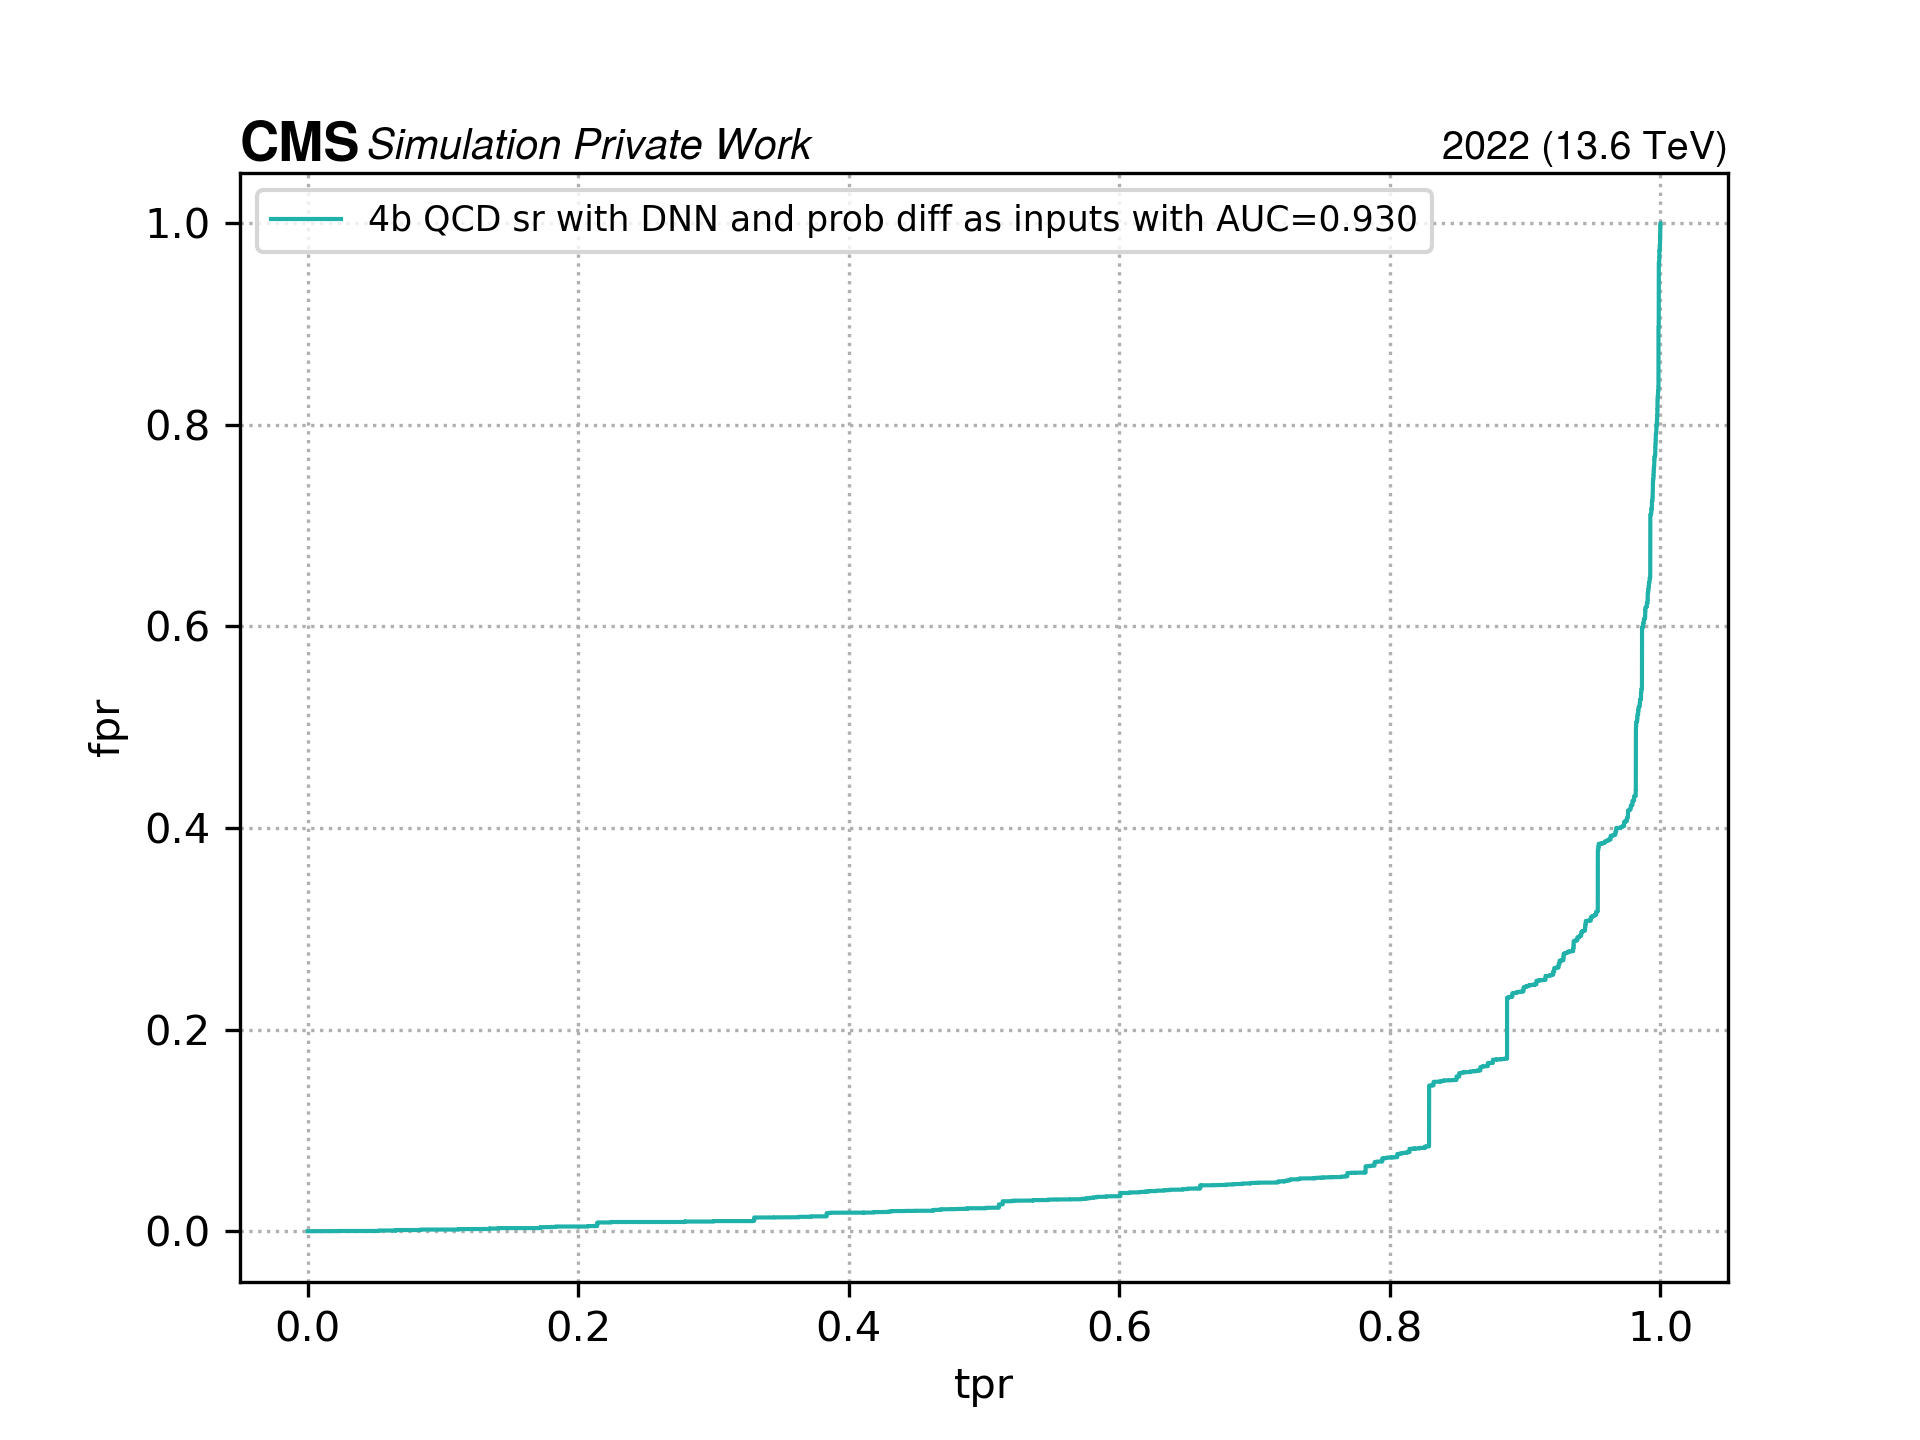
\includegraphics[width=0.7\linewidth]{Images/7.S:B/SR stats/ROC 4b QCD SR dnn proba.png}
    \caption{ROC of the assignment probability distribution obtained after a training and evaluation on SR samples shown in Figure \ref{fig: Assigned prob 4b QCD SR}}
    \label{fig: ROC of the assignment proba SR}
\end{figure}

Since in section \ref{subsection: var of training S/B}, we observed a large variability for the 4b-QCD configuration, we decided to test the variability of the the 4b-QCD-SR configuration trainings. We show the outcome of these trainings in Figure \ref{fig: 4b QCD SR variability} and in Table \ref{table: Spread of 4b QCD SR} we summarize the results. 

\begin{figure}[hbt]
\centering
\begin{subfigure}{.5\textwidth}
  \centering
  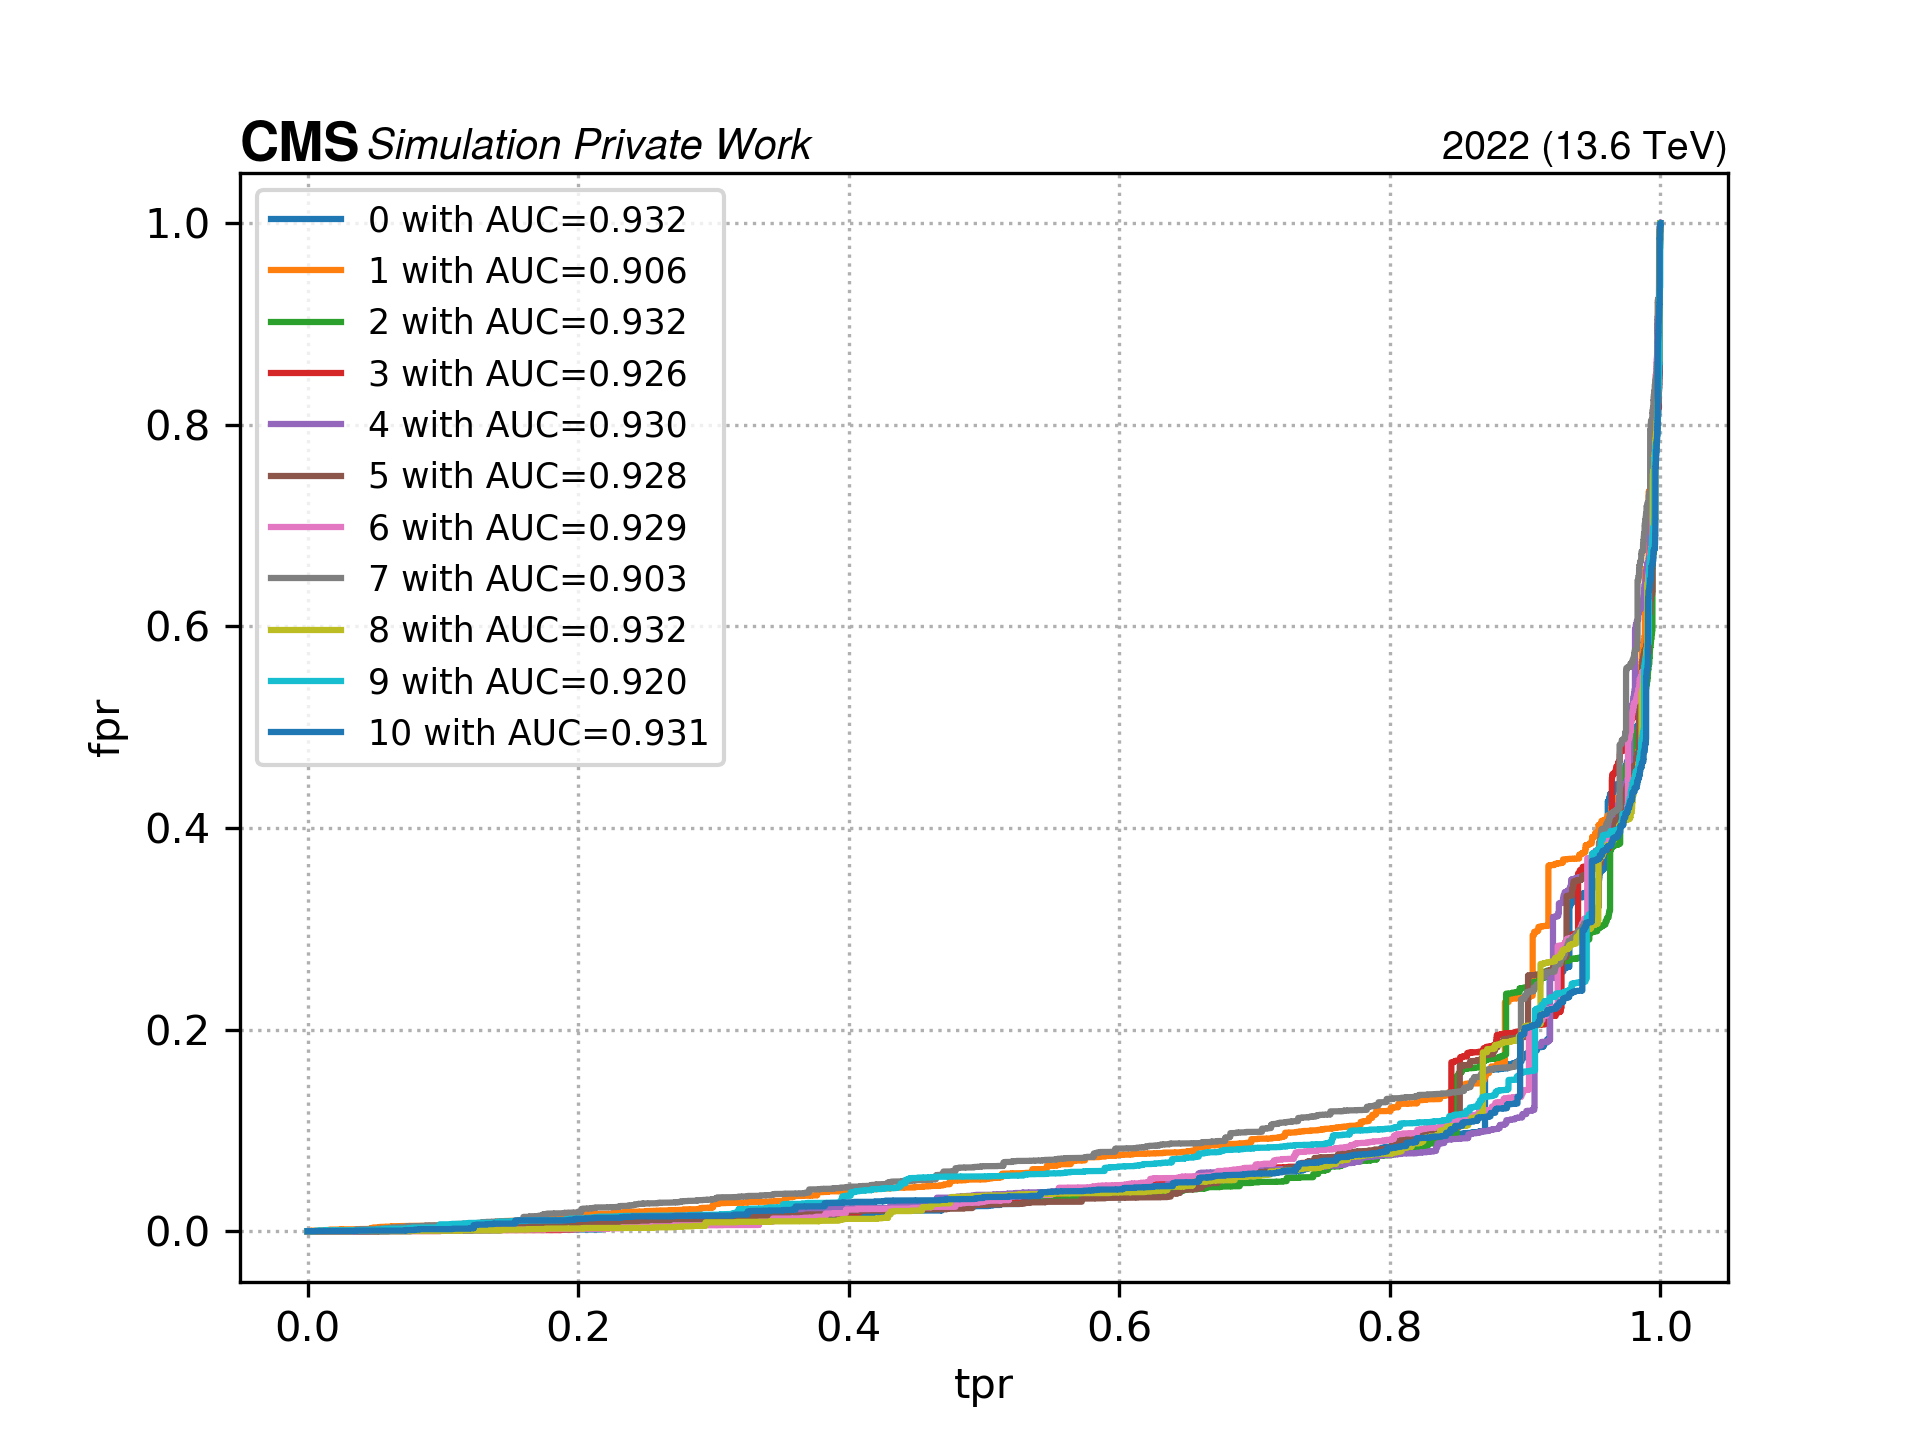
\includegraphics[width=1.1\linewidth]{Images/7.S:B/Variability/4b QCD sr dnn.png}
  \caption{DNN as global input}
  \label{fig: 4b QCD SR DNN}
\end{subfigure}%
\begin{subfigure}{.5\textwidth}
  \centering
  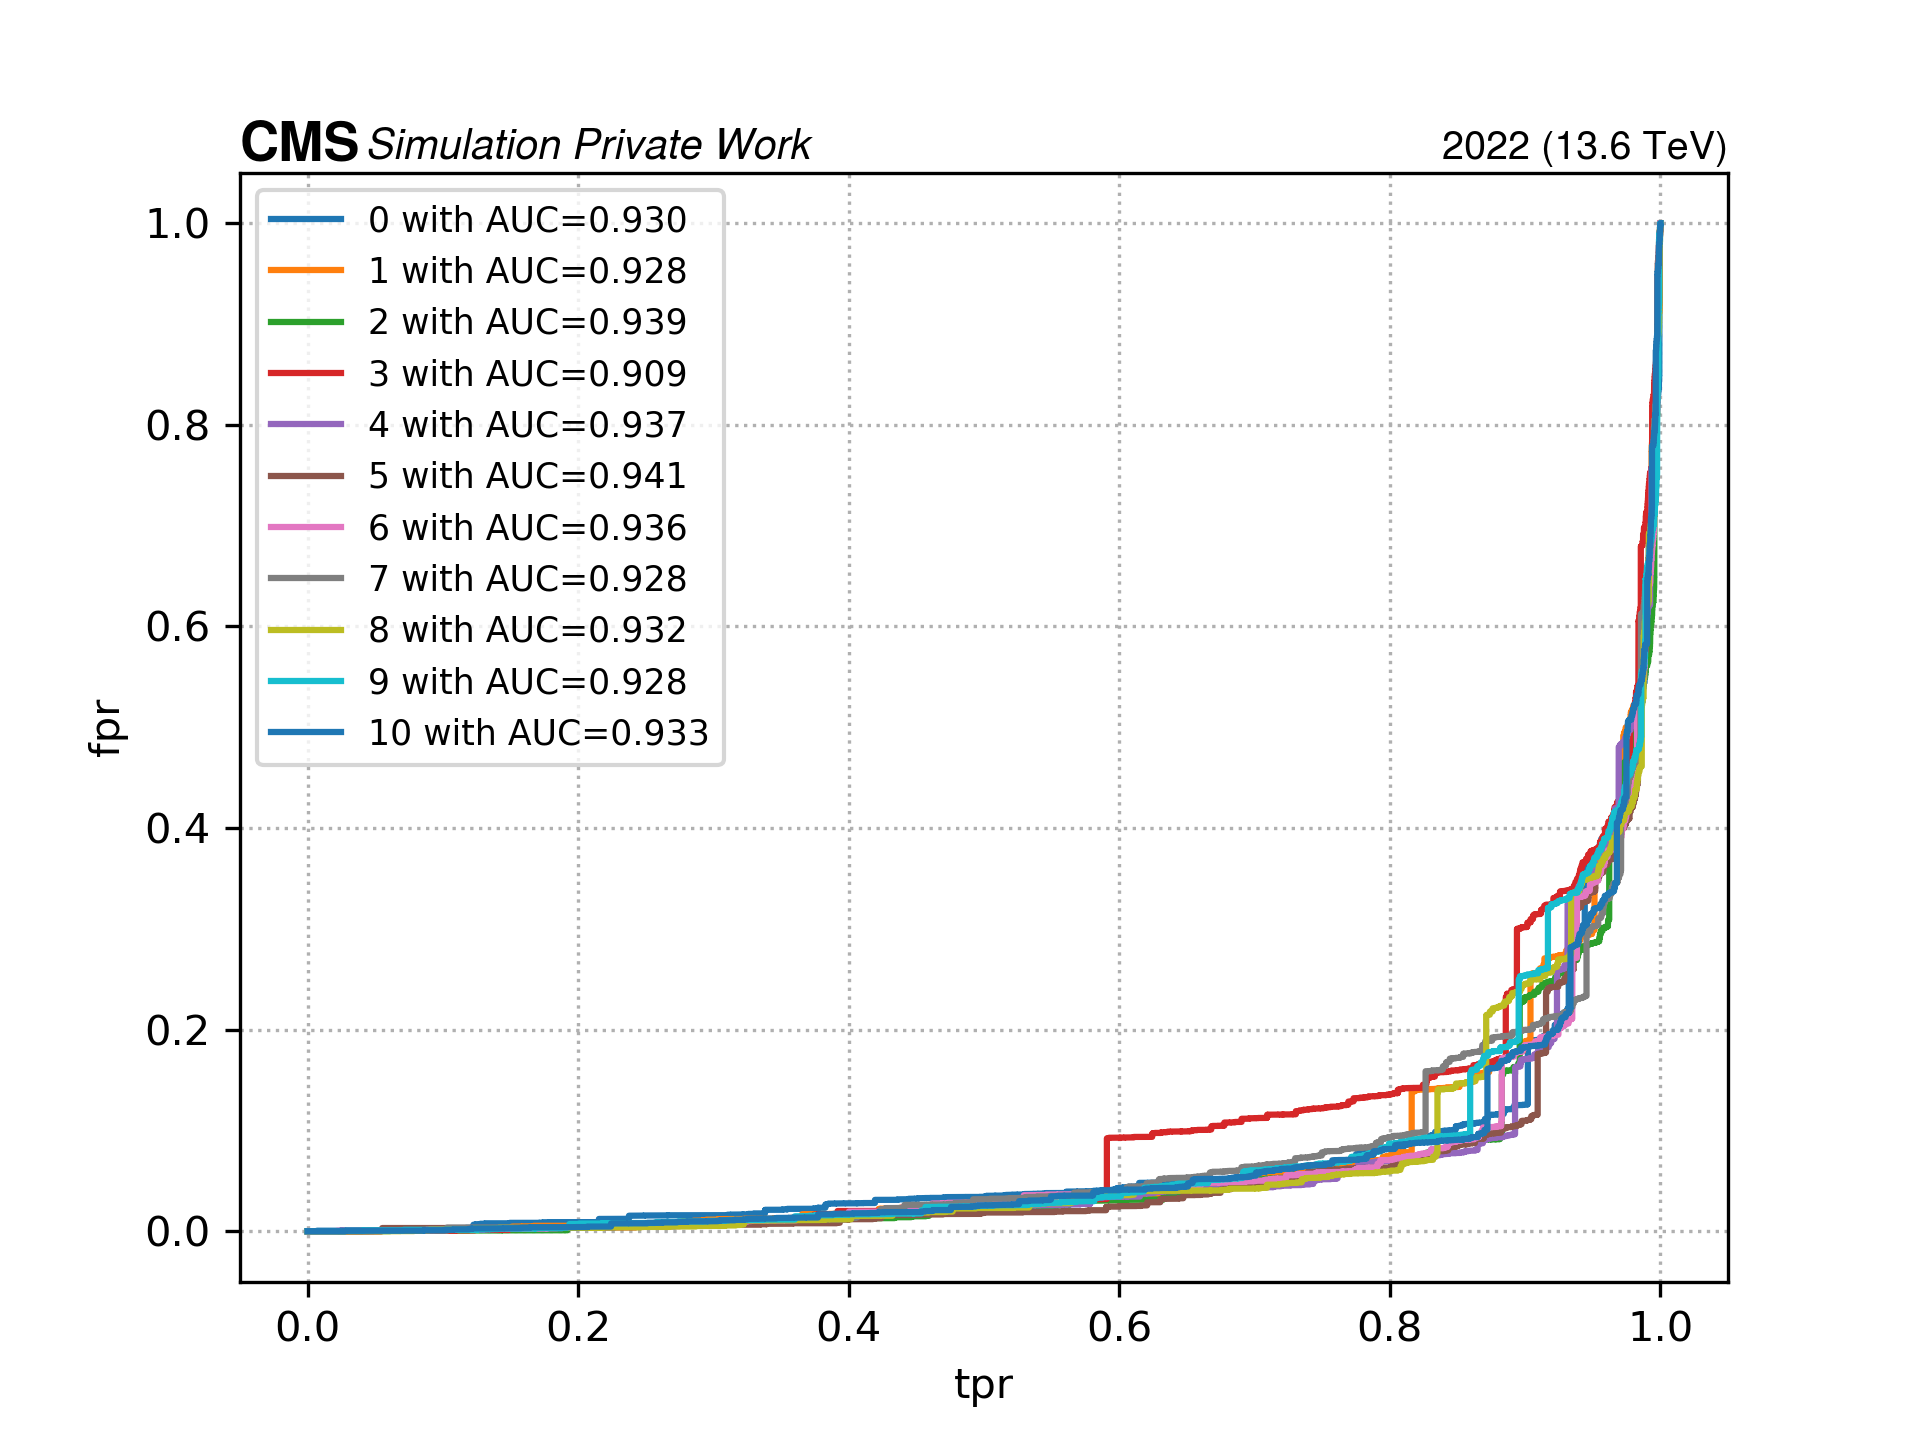
\includegraphics[width=1.1\linewidth]{Images/7.S:B/Variability/4b QCD sr dnn + prob diff.png}
  \caption{DNN and PD as global inputs}
  \label{fig: 4b QCD SR DNN PD}
\end{subfigure}
\caption{4b-QCD SR variability for the different inputs presented in Table \ref{table: S/B trainings}}
\label{fig: 4b QCD SR variability}
\end{figure}

\begin{table}[hbt]
\centering
\begin{tabular}{|M{5cm}||M{2.5cm}|M{2.5cm}|M{2.5cm}|}
 \hline
 Configuration  & Maximum value of the AUC & Minimum value of the AUC & Spread \\
 \hline
 4b-QCD-SR (DNN) & 0.932 & 0.903 & $\sim$0.029 \\
 \hline
 4b-QCD-SR (DNN and PD) & 0.941 & 0.909 & $\sim$0.033 \\
 \hline
\end{tabular}
\caption{Summary of the variability of the ROC and AUC values of the training for 4b-QCD SR training}
\label{table: Spread of 4b QCD SR}
\end{table}

As can be seen in Table \ref{table: Spread of 4b QCD SR}, we have an even higher variability than the one presented in section \ref{subsection: var of training S/B}, which can be explained by the lack of statistics of the background. Therefore, for the extrapolation for 4b-data in SR, we will do the same as in section \ref{subsection: var of training S/B}, and compute the b-tag ratio in Eq.(\ref{eq: extrapolation}) for the 11 seeds and see where the value from the AN
stands within this variability. The results are shown in Figures \ref{fig: 4b QCD SR DNN PD roc} and \ref{fig: 4b QCD SR DNN roc}. IN the SR we can conclude that adding the PD variable adds more variability to the trainings as previously noticed, however, adding this variable in the SR allows us to significantly improve our performance.

\begin{figure}[hbt]
    \centering
    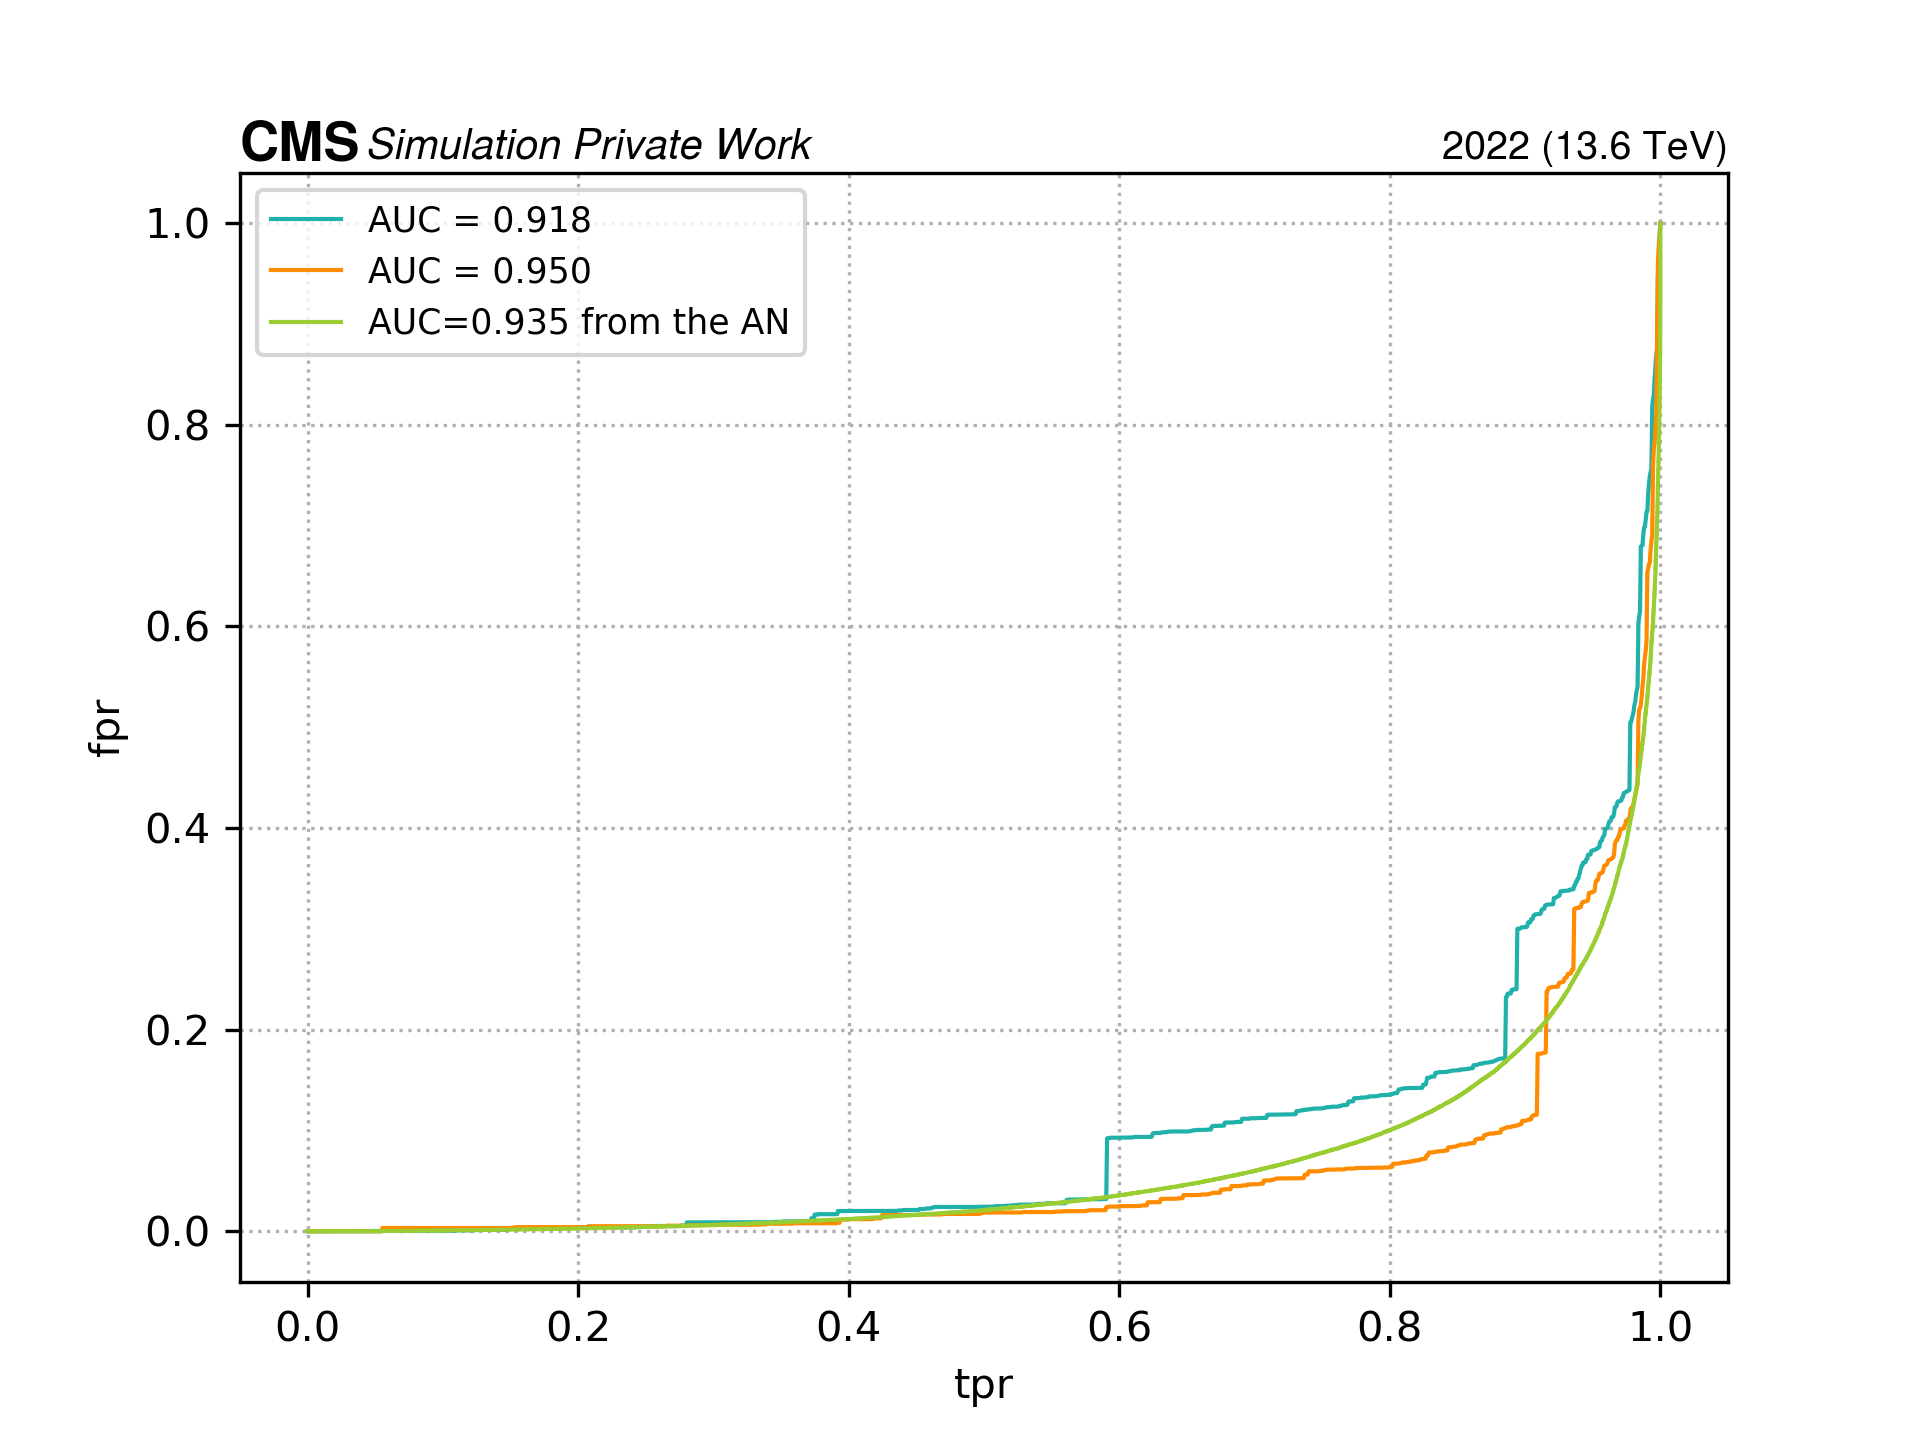
\includegraphics[width=0.7\linewidth]{Images/7.S:B/SR stats/4b data DNN + pb sr.png}
    \caption{4b-data in SR extrapolated ROC using the 4b-QCD-SR, 2b-data-SR full statistics, 2b-data-SR reduced statistics and 2b-QCD-SR configurations using DNN and PD as inputs. Here the AUC corresponds to the extrapolated AUC computed using Eq.(\ref{eq: extrapolation}).  Only the best and the worst performing trainings are shown in this figure to see more clearly where does the AN ROC stand within the variability of our training}
    \label{fig: 4b QCD SR DNN PD roc}
\end{figure}

\begin{figure}[hbt]
    \centering
    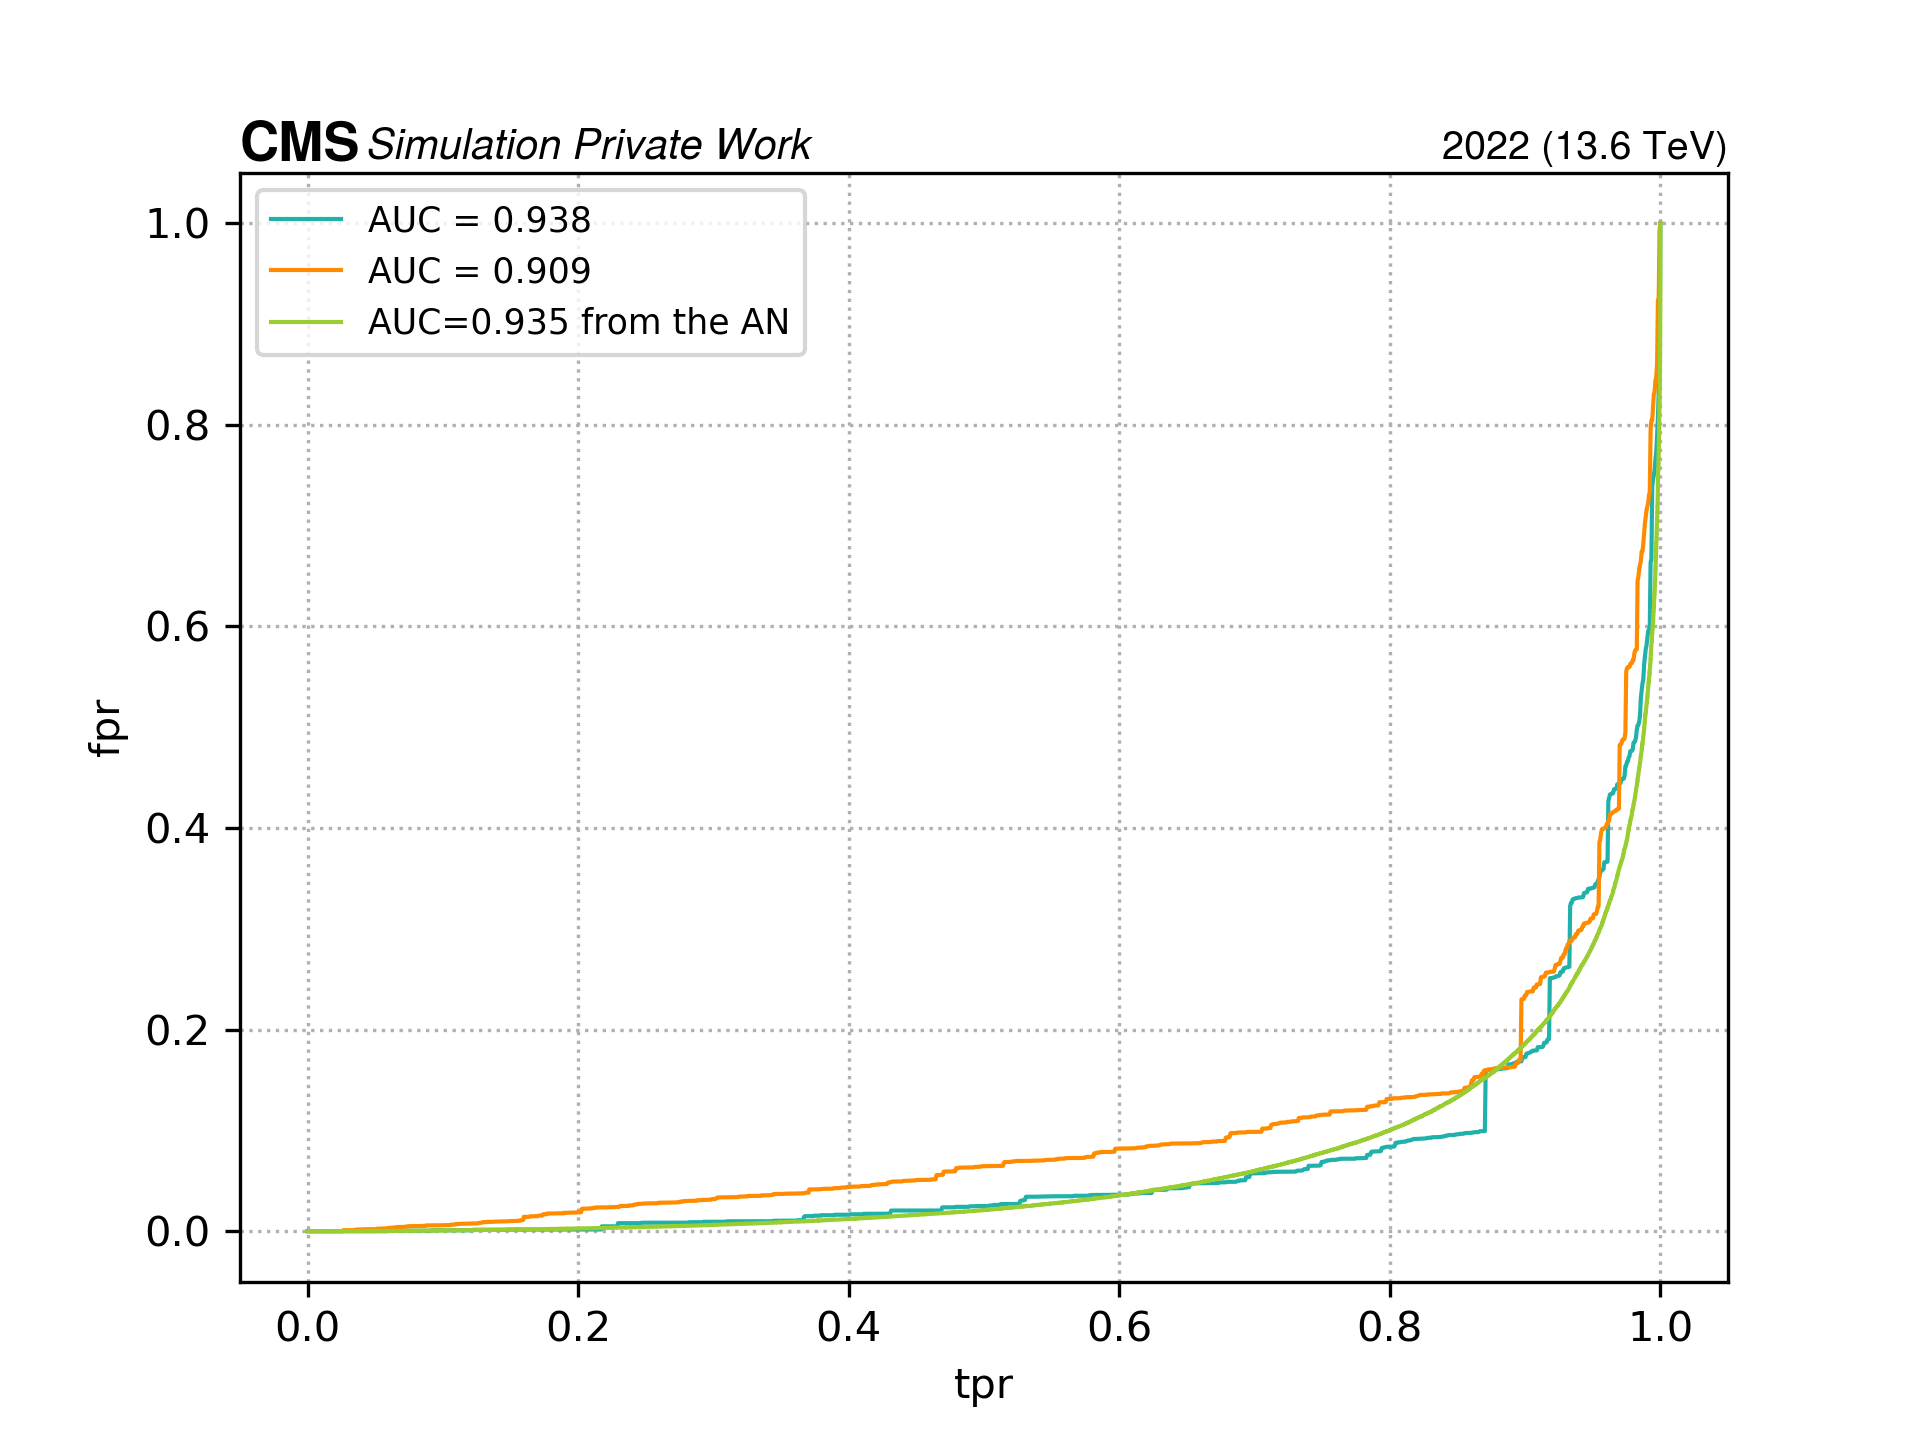
\includegraphics[width=0.7\linewidth]{Images/7.S:B/SR stats/4b data DNN.png}
    \caption{4b-data in SR extrapolated ROC using the 4b-QCD-SR, 2b-data-SR full statistics, 2b-data-SR reduced statistics and 2b-QCD-SR configurations using DNN as inputs. Here the AUC corresponds to the extrapolated AUC computed using Eq.(\ref{eq: extrapolation}).  Only the best and the worst performing trainings are shown in this figure to see more clearly where does the AN ROC stand within the variability of our training}
    \label{fig: 4b QCD SR DNN roc}
\end{figure}

We conclude by looking at Figures \ref{fig: highest comp} and \ref{fig: lowest comp} seeing the summarized results in Table \ref{table: highest/ lowest SR 4b data}, that by training our model using the DNN and PD as global inputs, 0.015 is the smallest gain that we get from this method, as here we only tested the variability with 11 seeds. Moreover, by using this training, our worse performance does not outperform the DNN used in Run 2, but is still better than the one using only DNN variables as global inputs. For the next steps, in order to avoid the lack of statistics and reduce the variability, we propose to oversample the 4b-QCD-SR sample used for the training.

\begin{table}[hbt]
\centering
\begin{tabular}{|M{5cm}||M{2.5cm}|M{2.5cm}|}
 \hline
 Configuration  & Maximum value of the AUC & Minimum value of the AUC \\
 \hline
 4b-data-SR (DNN) & 0.938 & 0.909  \\
 \hline
 4b-data-SR (DNN and PD) & 0.950 & 0.918 \\
 \hline
\end{tabular}
\caption{Comparison of the highest and lowest extrapolated AUC values for 4b-data using Eq.(\ref{eq: extrapolation}) to compute them. Here wee compare the difference given by the inputs in the training.}
\label{table: highest/ lowest SR 4b data}
\end{table}

\begin{figure}[hbt]
    \centering
    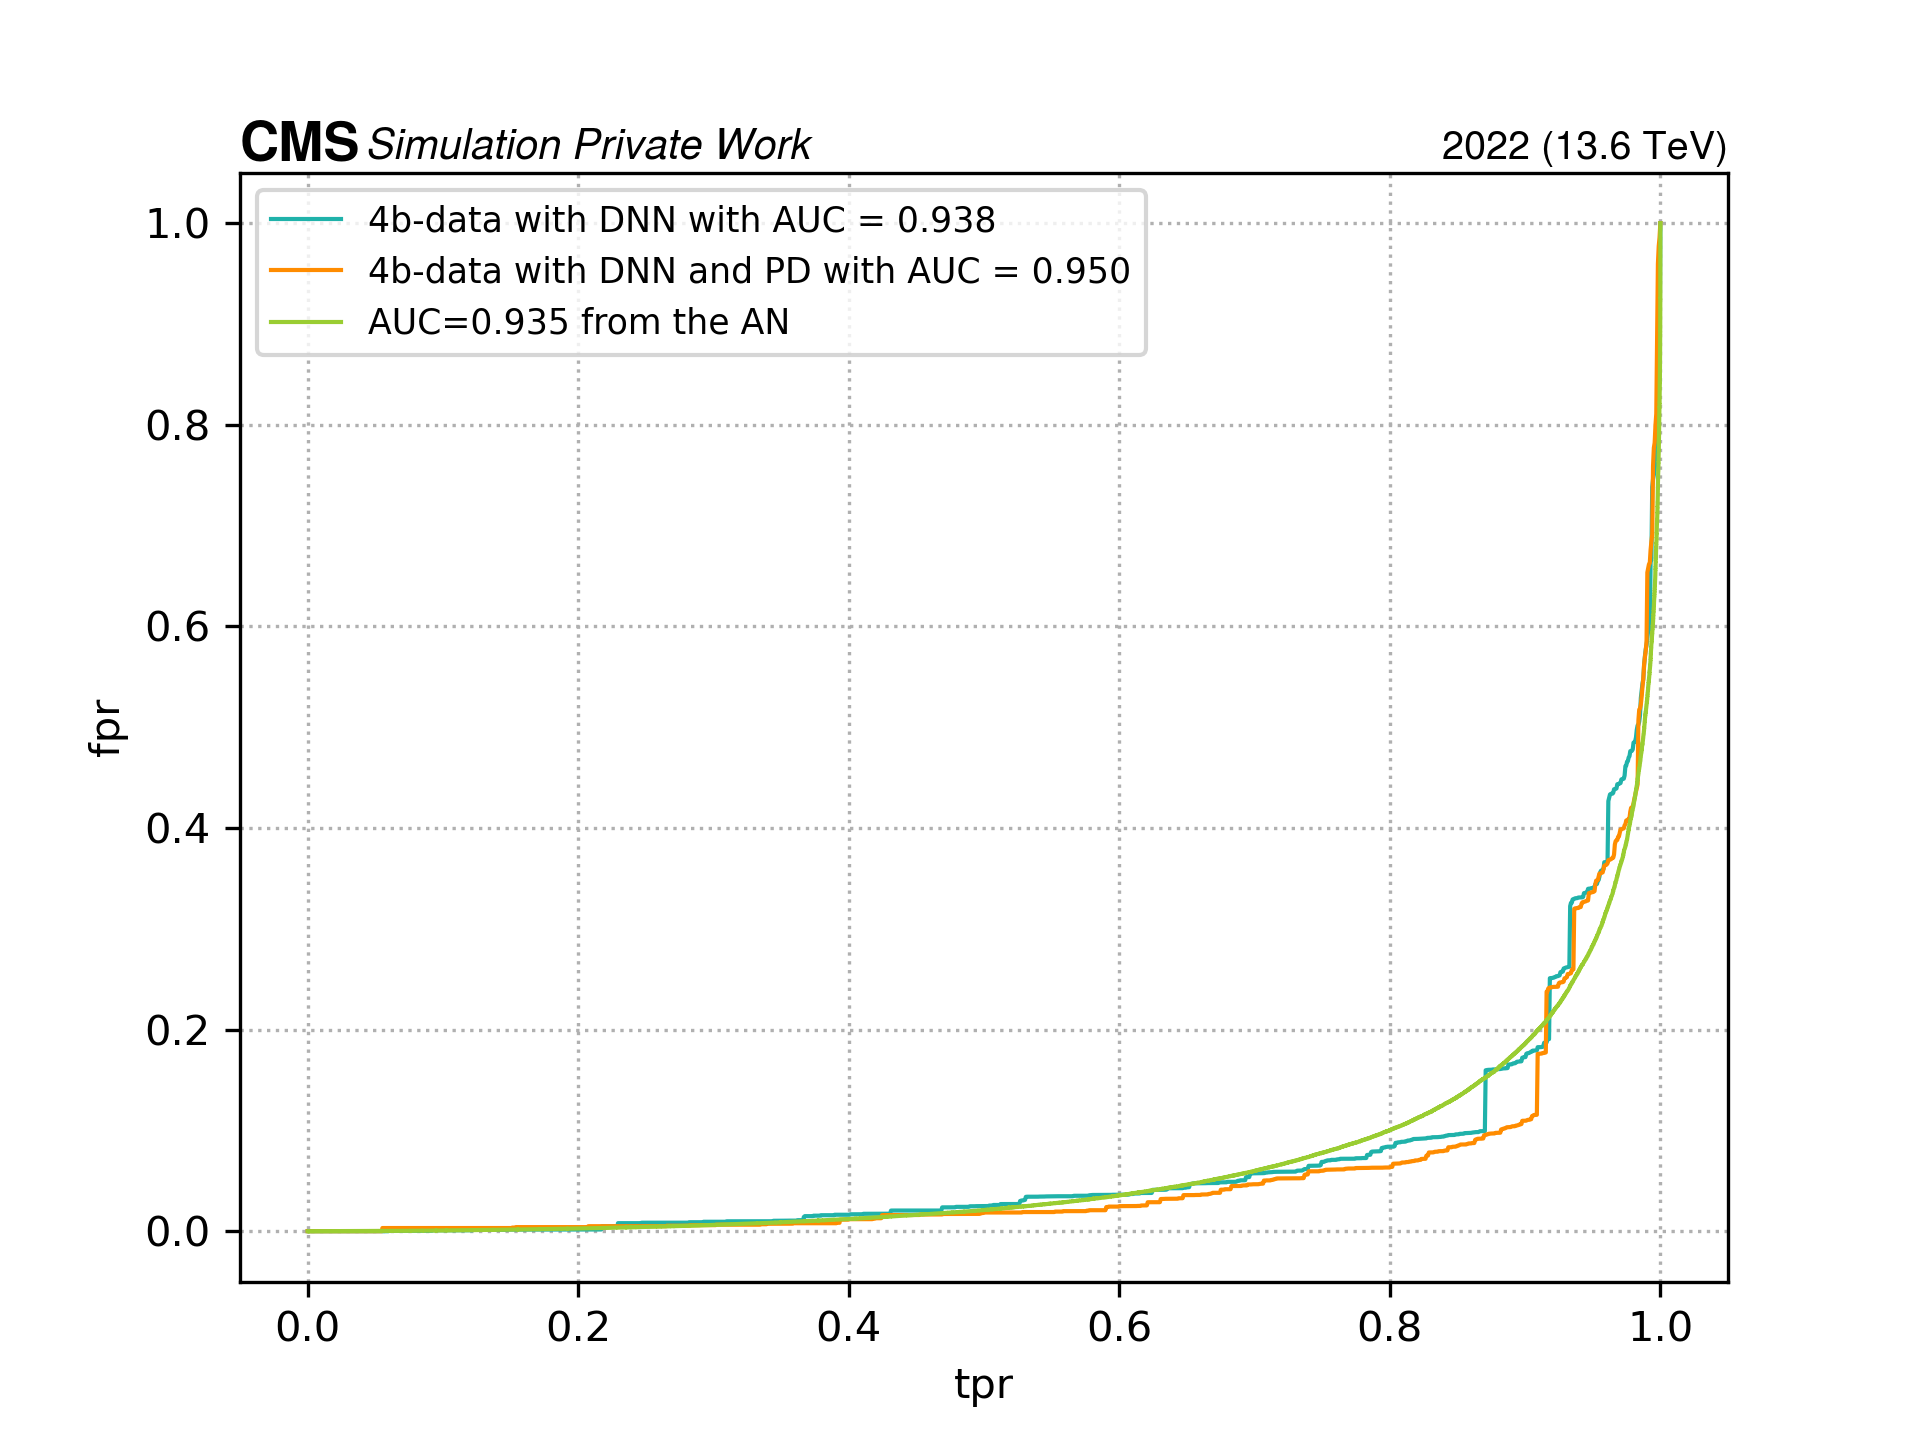
\includegraphics[width=0.7\linewidth]{Images/7.S:B/SR stats/HIghest AUC ROC vs Highest AUC vs AN.png}
    \caption{Comparison of the best performing 4b-data-SR extrapolated ROC when using either DNN as input variables or DNN as PD variables. The AUCs showed in this figure are the extrapolated using Eq.(\ref{eq: extrapolation}}
    \label{fig: highest comp}
\end{figure}

\begin{figure}[hbt]
    \centering
    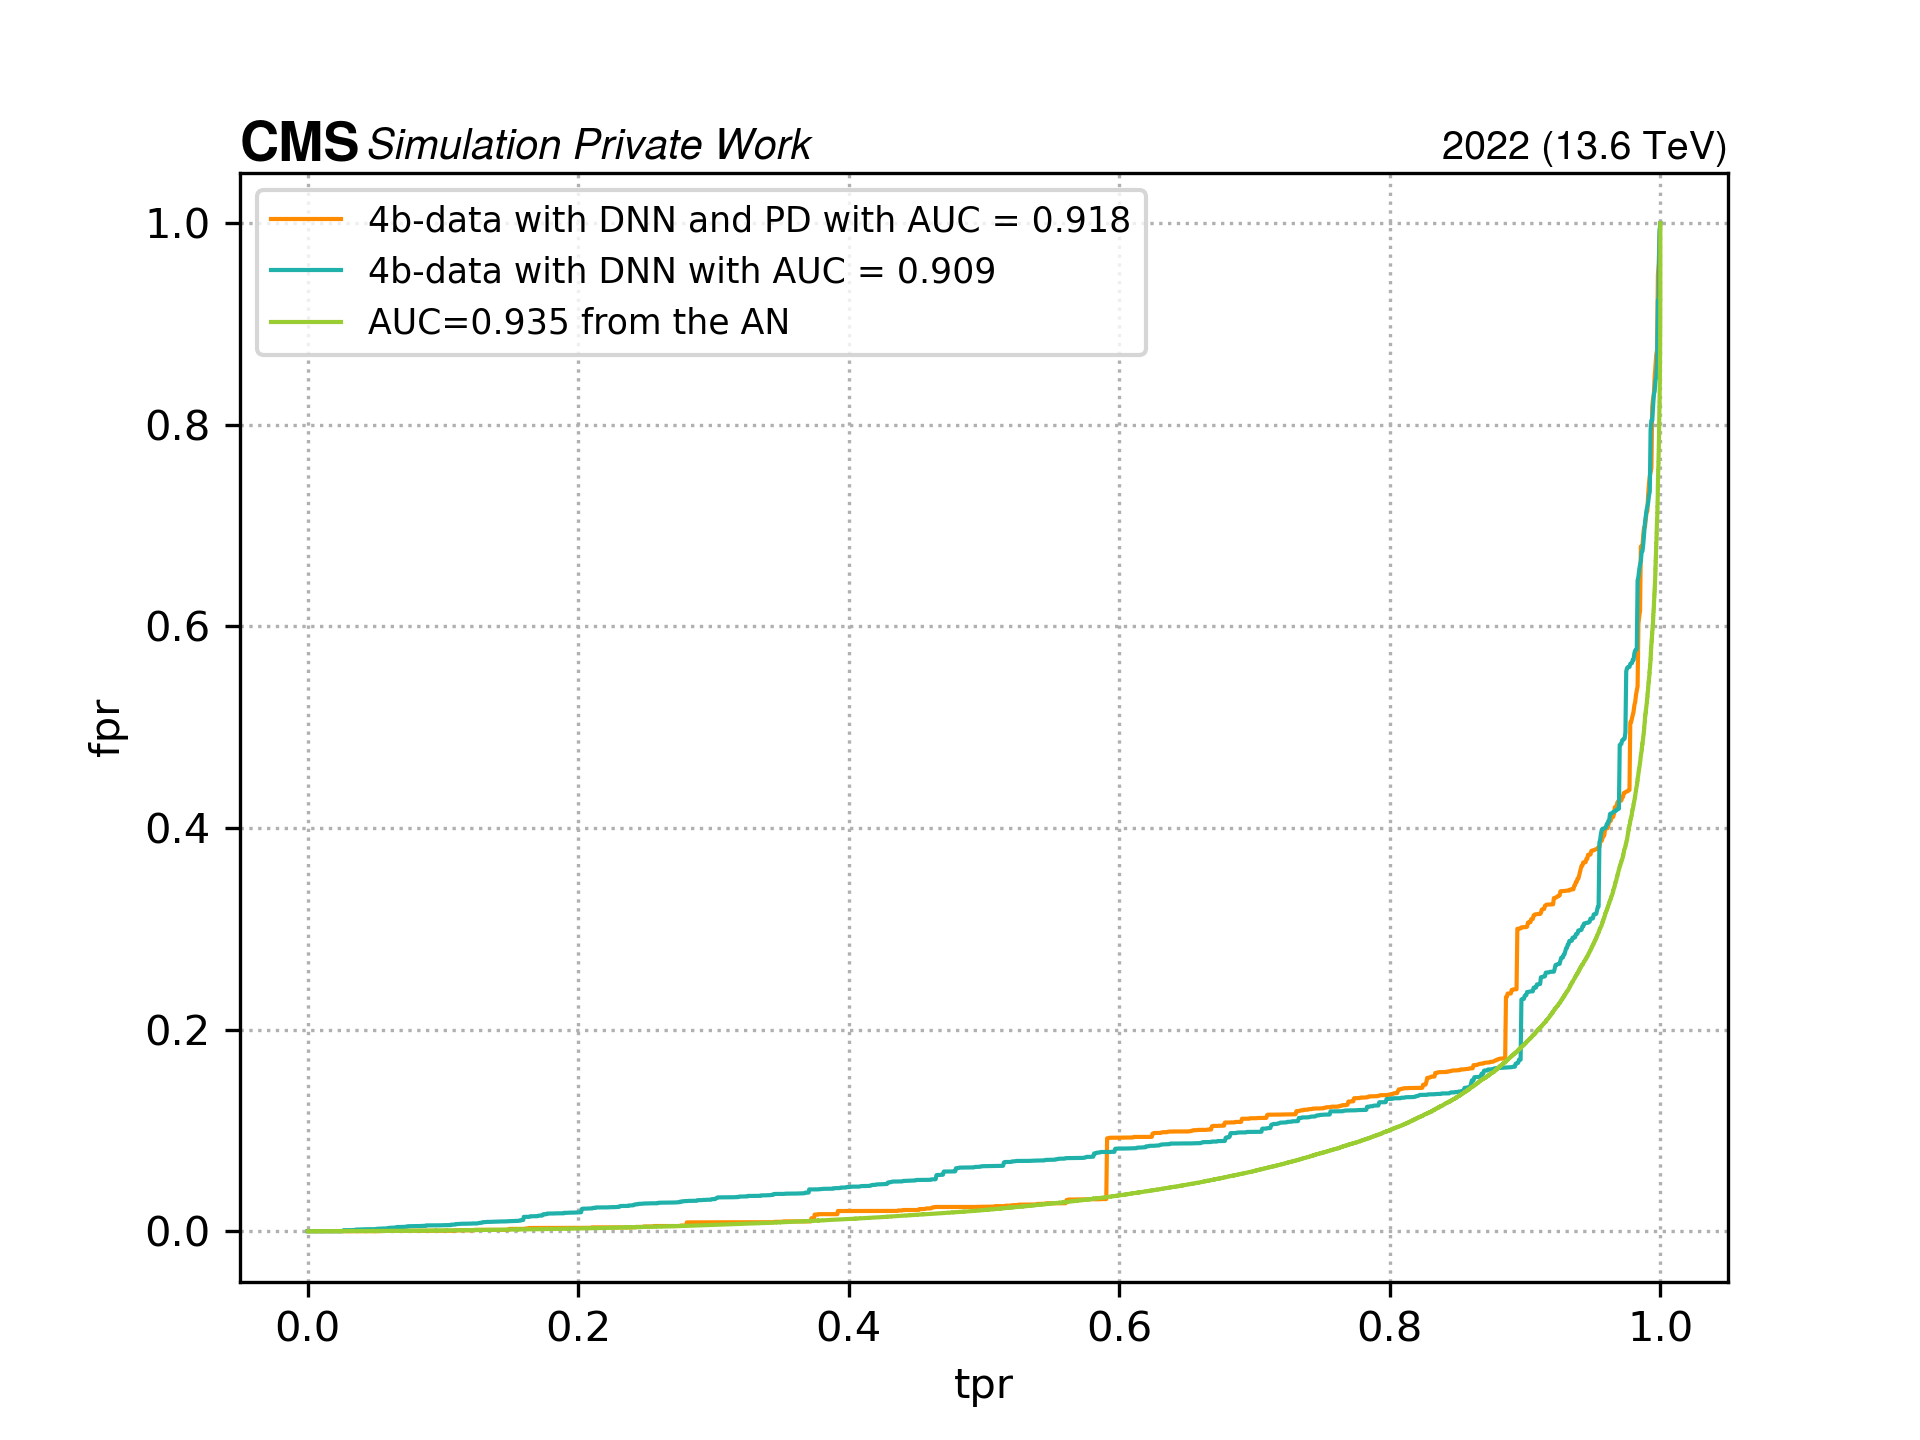
\includegraphics[width=0.7\linewidth]{Images/7.S:B/SR stats/lowest comp 4b data.png}
    \caption{Comparison of the worst performing 4b-data-SR extrapolated ROC when using either DNN as input variables or DNN as PD variables. The AUCs showed in this figure are the extrapolated using Eq.(\ref{eq: extrapolation})}
    \label{fig: lowest comp}
\end{figure}


Compare as a function of TPR saying that we outperform up tp 0.85 signal eff. after dominated by bckg, mention again the pb of stats . oversampling will play an important role